\documentclass{article}
\usepackage{newunicodechar}
\usepackage[OT1]{fontenc}
\usepackage{mathpazo}

\usepackage[italian]{babel}
\usepackage{caption}
\usepackage[dvipsnames]{xcolor}
\usepackage{fancyhdr}
\fancyhead{}
\renewcommand{\headrulewidth}{0pt} % Width of line at top of page
\fancyhead[L]{\leftmark} % Mark right [R] of page with Chapter name [\leftmark]

\pagestyle{fancy} % Set default style for all content pages (not TOC, etc)

%Prefisso della caption delle figure
\captionsetup[figure]{}% redefines the caption setup of the figures environment in the beamer class.

\usepackage{amsmath}
\usepackage{amsfonts}
\usepackage[utf8]{inputenc}
\usepackage{graphicx}
\usepackage{float}
\usepackage{hyperref}
\hypersetup{
    colorlinks,
    citecolor=black,
    filecolor=black,
    linkcolor=black,
    urlcolor=black
}
%Codice
\usepackage{listings}
\usepackage{algpseudocode}
\usepackage{algorithm}
\usepackage{booktabs}
\usepackage{amssymb}

\usepackage{chngcntr}
\counterwithin{figure}{section}


\newcommand{\ovcal}[1]{\overline{\mathcal{#1}}}

\title{\textbf{Algoritmi Euristici}}
\author{Manuel Pagliuca}

\begin{document}

\maketitle
\pagebreak
\tableofcontents
\pagebreak
\section{Introduzione}
L'obiettivo di questo corso è quello di mostrare che gli \textbf{algoritmi euristici} non sono ricette per problemi specifici:
le euristiche e i problemi possono essere combinati liberamente.
Una qualsiasi euristica può essere utilizzata su un qualsiasi problema. \textit{Euristica} è una parola che deriva dal Greco,
e sta per \textit{"metodologia di ricerca della verità o dei fatti"}, deriva da \textit{heurìsko} che significa \textit{io trovo}.

Il termine deriva da una storia molto famosa di Archimede, che aveva da risolvere il problema di imparare se la data corona d'oro era effettivamente
d'oro o se fosse solo placcata in oro. Questo era possibile da dedurre conoscendo il rapporto tra peso e volume, però il peso era facile da ottenere,
mentre il volume è molto più difficile.

L'idea di Archimede consisteva nell'utilizzo di un secchio colmo di acqua ed immergendo la corona in quest'ultimo, il quantitativo di acqua che esce
dal secchio consiste nel volume della corona.
\section{Algoritmi euristici}
\subsection{Cenni sulla parola}
La parola \textit{euristica} può cambiare di significato in base al campo in cui viene utilizzata, in alcuni settori scientifici la parola \textit{algoritmo euristico}
è considerata come \textbf{ossimoro} in quanto le due parole vengono considerate opposti.
\begin{itemize}
    \item \textbf{Algoritmo} ha un significato che sta per \textit{procedura deterministica} e \textit{formale}, la quale consiste in una sequenza finita di step elementari.
    \item \textbf{Euristico} ha un significato che sta per \textit{informale, creativo} e \textit{metodo a "regola aperta"} per trovare una soluzione.
\end{itemize}

Ogni algoritmo ha (od è) una \textbf{dimostrazione di correttezza} mentre un algoritmo euristico non ne ha nessuna.
Essi sono trasformazioni meccanico-simboliche che partono da uno \textit{starting point} (chiamato \textit{ipotesi}) e giungono ad un \textit{end point}(chiamato \textit{tesi}).

\subsection{Definizione}
Gli algoritmi euristici sono procedure formali dove la soluzione non è garantita essere quella \textbf{corretta}. Questo potrebbe sembrare inutile,
ma al contrario potrebbe essere utile per diversi motivi:
\begin{enumerate}
    \item \textbf{Costa} molto meno di un algoritmo corretto, in termini di \textit{spazio} e \textit{tempo}.
    \item Frequentemente \textbf{restituisce} qualcosa di \underline{vicino} alla soluzione corretta.
\end{enumerate}

Per definire la \textit{vicinanza} della soluzione, lo \textbf{spazio delle soluzioni} sarà dotato di una \textit{metrica} per esprimere una \textit{distanza soddisfacente}
della soluzione corrente dalla soluzione corretta.
Inoltre sarà dotato di una \textbf{distribuzione probabilistica} per esprimere la frequenza soddisfacente delle soluzioni che si trovano ad una distanza soddisfacente dalla
soluzione corretta (ovvero esprime quanto spesso l'algoritmo restituisce una soluzione soddisfacente).

\subsection{Motivazioni per gli algoritmi euristici}
Le euristiche sono la costruzione sia delle \textbf{dimostrazioni} che degli \textbf{algoritmi}, in caso di successo l'euristica viene abbandonata e la
\textit{dimostrazione} viene preservata. Altrimenti, una buona euristica solitamente porta ad un buon risultato, seppur non perfetto.
\section{Classificazione dei problemi}
Questo corso è incentrato su gli algoritmi euristici applicati ai problemi di \textbf{ottimizzazione combinatoria} che sono \textbf{basati su soluzioni}
(contrapposti a quelli \textbf{basati sui modelli}).

Un problema è una domanda che viene effettuata su un \textbf{sistema matematico}, la tipologia dei problemi viene classificata in base alla natura delle loro soluzioni.
\begin{enumerate}
    \item \textbf{problemi di decisione}: la loro soluzione è un booleano.
    \item \textbf{problemi di ricerca}: la loro soluzione è un qualsiasi sottoinsieme \textit{fattibile}.
    \item \textbf{problemi di ottimizzazione}: la loro soluzione è un numero il quale è il \textit{minimo} o \textit{massimo} valore di una \textbf{funzione obiettivo}
          definita su dei sottoinsiemi fattibili.
    \item \textbf{problemi di conteggio}: la loro soluzione è il \textit{numero} di sottoinsiemi \textit{fattibili}.
    \item \textbf{problemi di enumerazione}: la loro soluzione è la collezione di tutti i sottoinsiemi \textit{fattibili}.
\end{enumerate}
I problemi di ottimizzazione possono essere combinati con i problemi di ricerca, noi ci concentreremo su questo tipo di problemi, ovvero siamo alla ricerca del
\textbf{valore ottimale} e del \textbf{sottosistema che assume} quel valore.

\subsection{Problemi di ottimizzazione e ricerca}

Un problema di ottimizzazione e ricerca può essere rappresentato con:
$$opt_{x\in X}f(x)$$
Dove $x$ rappresenta una \textbf{sottosistema fattibile} che è una delle soluzioni, la quale soddisfa le condizioni fornite dal problema. Invece, $X$
è lo \textbf{spazio delle soluzioni fattibili}. Invece la funzione, si chiama \textbf{funzione obiettivo} ed è mappata in questa maniera $f:X \rightarrow R$,
il suo compito è quello di \textit{misurare quantitativamente} la qualità di ogni sottosistema (o soluzione).
Generalmente, in quanto problema di ottimizzazione, la funzione obiettivo è \textit{massimizzabile} o \textit{minimizzabile}, questo viene denotato con $opt\in {min,max}$.

Il problema consiste nel determinare il \textbf{valore ottimale della funzione obiettivo} assieme alla \textbf{soluzione ottima} tale che sia un sottoinsieme.
Il valore ottimale della funzione obiettivo viene chiamato $f^*$, ed è il risultato della seguente equazione:
$$f^*=opt_{x\in X}f(x)$$
Ovvero un valore che consiste nel minimo o massimo della funzione obiettivo. Mentre, la soluzione ottima tale che sia un sottoinsieme si chiamerà $x^*$:
$$x^*\in X^*=arg\textit{ } opt_{x\in X}f(x)={x^* \in X : f(x^*)=opt_{x\in X}f(x)}$$
Ovvero, vogliamo trovare una soluzione ottima nell'intero insieme di tutte le soluzioni ottime, anche se solitamente una è abbastanza, la notazione $arg$
sta per l'intero insieme delle soluzioni (ne basta una).

\subsection{perché siamo interessati nei problemi di ottimizzazione e ricerca ?}

I problemi di ottimizzazione e ricerca sono di forte interesse poiché diversi campi applicativi richiedono oggetti o strutture caratterizzati da valori molto alti o molto bassi rispetto ad una propria funzione di valutazione.
\begin{itemize}
    \item Bioinformatica
    \item Social networks
    \item Machine learning
    \item Hardware design
    \item Stima dei parametri
    \item Finanza
\end{itemize}

L'\textbf{ottimizzazione esatta} è costosa da un punto di vista computazionale e non sempre desiderabile (per questo gli algoritmi euristici sono favoriti);
perciò, solitamente, le funzioni di valutazione sono delle \textit{approssimazioni} di quello che realmente accade. In questo corso assumeremo il punto di vista dell'ottimizzazione, cercando di ottimizzare al meglio possibile la funzione obiettivo.

Diversi problemi possono spesso essere ridotti in problemi di ottimizzazione e ricerca
\begin{itemize}
    \item \textit{Problemi di ricerca} possono essere ridotti rilassando le condizioni da soddisfare, in maniera da allargare la \textbf{regione di fattibilità}
          da $X$ a $X'\supset X$ ed ottenere un problema di ricerca semplice. Si introduce una funzione $d(x)$ per quantificare la distanza di ogni soluzione $x\in X'$ da $X$. Infine, minimizzando $d(x)$ per trovare $x^*$ tale che $d(x^*)=0 \Leftrightarrow x^* \in X$.
    \item Alcuni \textit{problemi di decisione} riguardano l'esistenza di sottosistemi fattibili, e sono identici ai problemi di
          ricerca (trovare il sottosistema dimostra la sua esistenza).
    \item Alcuni \textit{problemi di numerazione} riguardano la ricerca di sottosistemi con \textit{"buoni"} valori di funzioni oggettive in conflitto e permettono
          \textit{adattamenti diretti} ad algoritmi di ottimizzazione e ricerca.
\end{itemize}
Tali riduzioni sono spesso possibili ed utili, ma non sempre.
\subsection{Problema di ottimizzazione combinatoria}
Un problema è un problema CO (\textit{Combinatorial Optimization}) quando la regione di fattibilità \textit{X} è un insieme finito, e quindi, che abbia un numero
finito di \textit{soluzioni fattibili}. Questa sembra un'assunzione molto restrittiva, ma sono presenti molti
problemi che hanno un numero infinito di soluzioni che possono essere ridotti a problemi che hanno un numero finito di soluzioni.

Per esempio:
\begin{itemize}
    \item I problemi infiniti nel discreto possono avere un insieme finito di soluzioni interessanti.
    \item Alcuni problemi continui possono essere ridotti a problemi di ottimizzazione combinatoria: \textit{Programmazione lineare, Flusso massimo, Costo minimo di flusso, ...}.
    \item I problemi continui possono essere ridotto in discreto utilizzando il campionamento (solitamente non è molto efficace).
    \item Le idee concepite per i problemi CO possono essere estese ad altri problemi.
\end{itemize}

\subsection{Euristiche basate sui modelli}
In questo corso parleremo solamente di \textbf{euristiche basate su soluzioni}, ma è importante conoscere anche la controparte.
L'euristiche basate sui modelli descrivono la regione di fattibilità $X$ con un "modello", un esempio tipico è una funzione matematica.
$$opt_{x\in X} f(x) \rightarrow \text{min}_{g_i(\xi)\leq 0}\phi(\xi) \text{ per } i=1,...,m$$

Dove $\xi \in \mathbb{R}^n$, il quale è il vettore delle soluzioni di $n$ numeri reali. Mentre $X={\xi \in \mathbb{R}^n : g_i(\xi)\leq 0, i=1,...,m}$, ovvero che la
regione di fattibilità è l'insieme dei vettori che soddisfanno tutte le disuguaglianze.
L'euristiche basate su modelli estrapolano l'informazione derivata dal modello, che sono le proprietà analitiche della funzione $\phi$ e $g_i \text{ per } i=1,...m$.

\subsection{Definizione alternativa di CO}
Una problema è un problema CO() quando:
\begin{enumerate}
    \item Il numero di soluzioni fattibili è finito (prima definizione).
    \item La regione di fattibilità è $X\subseteq 2^B$ per un dato \textbf{ground set} $B$, ovvero, le \textit{soluzioni fattibili} sono tutte sottoinsiemi del ground set che
          soddisfa le condizioni adeguate.
\end{enumerate}

Entrambe le definizioni sono equivalenti:
\begin{itemize}
    \item $2 \implies 1$: se il ground set $B$ è finito, ogni collezione $X\subseteq 2^B$ è finita.
    \item $1 \implies 2$: se il numero di soluzioni fattibili è finito, definire $B$ come il loro sovrainsieme ed $X$ la \textit{regione fattibile} sarà la
          collezione dei singoli elementi di $B$ (una \textit{"soluzione"} è un insieme contenente una singola soluzione).
\end{itemize}
In generale, la definizione sofisticata permette un analisi più profonda, perché $X$ non viene semplicemente numerato
e viene definito in una maniera \textit{compatta} e \textit{significativa}.

\subsection{Euristiche basate su soluzioni}
L'euristiche basate su soluzioni considerano le soluzioni come sottoinsiemi del ground set, esse possono essere classificate in:
\begin{enumerate}
    \item \textbf{Euristiche costruttive/distruttive}, iniziano da un sottoinsieme estremamente semplice
          (può essere $\emptyset$ o $B$), poi, esse aggiungono/rimuovono gli elementi fino a che non ottengono la soluzione desiderata.
    \item \textbf{Euristiche di scambio}, iniziano da un sottoinsieme ottenuto in una qualsiasi maniera,
          poi, scambiano gli elementi fino a che non ottengono la soluzione desiderata.
    \item \textbf{Euristiche di ricombinazione}, iniziano da una popolazione di sottoinsiemi ottenuta in una qualsiasi maniera,
          poi, ricombinando differenti sottoinsiemi produrranno una \textit{nuova} popolazione.
\end{enumerate}

I progettisti delle euristiche possono combinare in maniera creativa gli elementi delle diverse classi delle euristiche.

\subsubsection{Randomizzazione e memoria}
Sono presenti due cose importanti che intervengono nella progettazione di un algoritmo:
\begin{itemize}
    \item \textbf{Randomizzazione}
    \item \textbf{Memoria}
\end{itemize}

Puoi avere algoritmi che usano o non usano la randomizzazione o la memoria.
Questi due elementi sono ortogonali (indipendenti) rispetto alla classificazione delle euristiche basate sulle soluzioni, per ognuna di esse possiamo dire che abbiamo quattro sottoclassi.

\begin{enumerate}
    \item Utilizzo della randomizzazione:
          \begin{itemize}
              \item \textbf{Euristiche puramente deterministiche}
              \item \textbf{Euristiche \textit{"randomizzate"}}, essenzialmente sono algoritmi che utilizzano come input numeri pseudo-casuali.
          \end{itemize}
    \item Utilizzo della memoria:
          \begin{itemize}
              \item Euristiche dove l'input include solamente i \textbf{dati del problema}.
              \item Euristiche dove l'input include anche \textbf{soluzioni precedentemente generate}.
          \end{itemize}
\end{enumerate}

Comunemente si utilizza il termine \textit{metaeuristiche} (dal Greco, \textit{"oltre le euristiche"}) per descrivere gli algoritmi euristici
che vanno utilizzano la randomizzazione e/o la memoria.

\subsection{Rischi da cui stare attenti}
\begin{enumerate}
    \item \textbf{Attitudine reverenziale o alla tendenza}, ovvero, nello scegliere un algoritmo basato sul contesto sociale, anziché sul problema.
    \item \textbf{Attitudine magica}, ovvero, \textit{credere} in un metodo sulla base di un analogia con un fenomeno fisico e naturale.
    \item \textbf{Integralismo euristico}, ovvero, utilizzare un euristica per un problema che ammette l'utilizzo di un algoritmo esatto.
    \item \textbf{Sgranocchiare numeri}, ovvero, eseguire sofisticati e complessi calcoli con numeri inaffidabili.
    \item \textbf{Attitudine SUV}, ovvero, affidarsi alla potenza dell'hardware.
    \item \textbf{Complicare ulteriormente}, ovvero, introdurre componenti e parametri \textit{ridondanti}, per cercare (fallendo) di migliorare il risultato.
    \item \textbf{Overfitting}, ovvero, adattare i componenti ed i parametri dell'algoritmo ad un dataset specifico utilizzato nella valutazione sperimentale.
\end{enumerate}

Inoltre è fondamentale:
\begin{itemize}
    \item Liberarsi dai pregiudizi.
    \item Valutare le prestazioni dell'algoritmo in una maniera scientifica.
    \item Distinguere il contributo di ogni componente dell'algoritmo.
    \item Implementare efficientemente ogni componente dell'algoritmo.
\end{itemize}

\section{Problemi di ottimizzazione combinatoria}
Il ground set è la base sul quale si costruisce l'algoritmo, abbiamo visto che sono presenti molteplici possibilità con le
euristiche basate sulle soluzioni, la loro classe cambierà in base al ground set utilizzato.
Quindi per prima cosa dobbiamo capire che cosa è (\textit{tipologia}) il \textbf{ground set}.

Visiteremo inizialmente un certo numero di problemi, questo sarà utile perché:
\begin{itemize}
    \item Le idee astratte devono essere applicate concretamente su diversi algoritmi per diversi problemi.
    \item La stessa idea può avere differente efficacia su diversi problemi.
    \item Alcune idee funzionano solamente su problemi con una specifica struttura.
    \item Diversi problemi potrebbero non avere un apparente relazione, cosa che può essere sfruttata per progettare algoritmi.
\end{itemize}

Una buona conoscenza di diversi problemi ci insegna ad applicare le idee astratte a nuovi problemi e ci insegna come trovare e sfruttare le relazioni tra problemi conosciuti e nuovi.

\subsection{Insieme dei problemi pesati}
\subsubsection{Knapsack Problem (KP)}
Il problema dello zaino, \textit{Knapsack Problem}. Il problema consiste nell'avere a disposizione uno zaino che ha una \textit{capacità limitata} ed un insieme di oggetti con differenti
\textit{volumi} e \textit{valori}, si vuole riempire lo zaino con gli oggetti di valore massimo (ovviamente non si può mettere dentro tutti gli oggetti).

Dati:
\begin{itemize}
    \item Insieme elementare $E$ di oggetti.
    \item Una funzione $v:E\rightarrow \mathbb{N}$ che descrive il \textbf{volume} di ogni oggetto.
    \item Un numero $V\in \mathbb{N}$ che descrive la \textbf{capacità} dello zaino.
    \item Una funzione $\phi : E\rightarrow \mathbb{N}$ che descrive il \textbf{valore} di ogni oggetto.
\end{itemize}

Banalmente, il \textbf{ground set} è l'insieme degli oggetti $B\equiv E$. La \textbf{regione di fattibilità} include tutti i sottoinsiemi degli
oggetti il cui volume totale non eccede la capacità $V$ dello zaino.
$$X=\left\{x\subseteq B : \sum_{j\in x}v_j \leq V\right\}$$

L'obiettivo è quello di massimizzare il valore totale degli oggetti scelti:
$$max_{x\in X} f(x)=\sum_{j\in x}\phi_j$$

Per esempio, nella seguente tabella sono mostrati tutti gli elementi di $E$ con i relativi valori e volumi. Sapendo che lo zaino ha una capacità massima $V=8$, consideriamo due \textbf{soluzioni candidate}:

\begin{figure}[H]
    \centering
    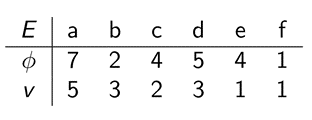
\includegraphics[width=6cm]{images/tab_KP.png}
    \caption{Dataset}
    \label{fig:tab_KP}
\end{figure}

\begin{figure}[H]
    \centering
    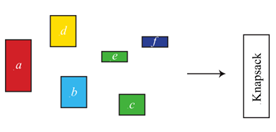
\includegraphics[width=6cm]{images/graphic_KP.png}
    \caption{Raffigurazione problema dello zaino}
    \label{fig:graphic_KP}
\end{figure}

\begin{figure}[H]
    \centering
    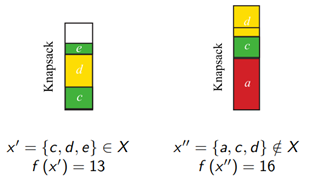
\includegraphics[width=8cm]{images/cand_sol_KP.png}
    \caption{Soluzioni candidate}
    \label{fig:cand_sol_KP}
\end{figure}

\begin{itemize}
    \item La prima soluzione candidata considera tre elementi la cui somma è $\leq V$, questo significa che la
          soluzione è un sottoinsieme preso dalla regione di fattibilità $X$ ed è una \textbf{soluzione fattibile}.
    \item La seconda soluzione candidata ha una somma di elementi pari a $10$, la quale è $>V$. Quindi questo sotto insieme
          non è appartenente alla regione di fattibilità $X$ (ma solo al ground set), perciò verrà chiamata \textbf{soluzione infattibile}.
\end{itemize}

Tra le soluzioni fattibili proposte la \textbf{funzione obiettivo} propone di prendere la soluzione \textit{massima}, ma visto che $x''$ non è fattibile, prenderemo come soluzione $x'$.
\subsubsection{Maximum Diversity Problem (MDP)}
Il problema della diversità massima, \textit{Maximum Diversity Problem}, è un problema importante per il corso e
verrà utilizzato come esempio per la parte di laboratorio. Questo è un problema
definito su uno spazio metrico, quindi uno spazio con la nozione di \textit{distanza}.

Dati:
\begin{itemize}
    \item Un insieme di punti $P$.
    \item Una funzione $d:P \times P \rightarrow \mathbb{N}$, la quale provvede la distanza tra le coppie di punti.
    \item Un numero $k\in {1,...,|P|}$, il quale è il numero di punti che si vuole selezionare.
\end{itemize}

Il problema chiede di selezionare da un insieme di punti $P$ un sottoinsieme di $k$ punti la cui sommatoria delle distanze tra le coppie dei punti sia massima.
Questo è un problema CO, perché il numero di sottoinsiemi possibili è finito, ed in particolare è un problema CO perché le soluzioni sono sottoinsiemi del ground set.
Il ground set, banalmente, è l'insieme dei punti $B\equiv P$, mentre la regione di fattibilità include tutti i sottoinsiemi composti da $k$ punti.
$$X=\left\{x\subseteq B : |x| = k \right\}$$
La funzione obiettivo è la sommatoria di tutte le distanze tra le coppie di punti in $x$:
$$max\underset{x\in X}{f(x)}=\sum_{(i,j):i,j\in x}d_{ij}$$

Per esempio, consideriamo un dataset costituito da $7$ punti e considerando un $k=3$, questo significa che vogliamo trovare
un sottoinsieme costituito da $3$ punti tale che le coppie abbiano distanza massima.

\begin{figure}[H]
    \centering
    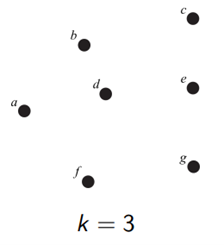
\includegraphics[width=3cm]{images/graph_MDP.png}
    \caption{Dataset}
    \label{fig:graph_MDP}
\end{figure}

\begin{figure}[H]
    \centering
    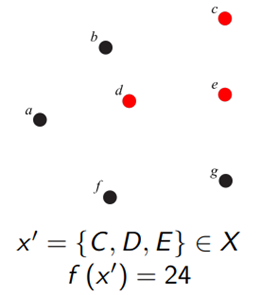
\includegraphics[width=3cm]{images/sol1_MDP.png}
    \caption{Prima soluzione candidata del MDP}
    \label{fig:cand_sol_MDP}
\end{figure}

\begin{figure}[H]
    \centering
    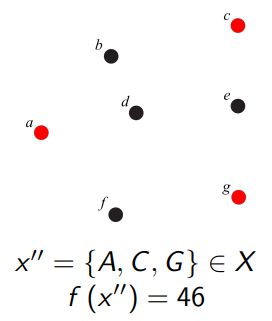
\includegraphics[width=3cm]{images/sol_MDP.png}
    \caption{Seconda soluzione candidata del MDP}
    \label{fig:cand_sol_2_MDP}
\end{figure}

La prima soluzione $x'$, considerando una metrica \textit{non fornita} ha come valutazione della funzione obiettivo $f(x')=24$, ed è un sottoinsieme tale per cui
la sua cardinalità sia $\leq k$, e quindi appartenente alla regione di fattibilità $X$.

La seconda soluzione ha come soluzione della funzione obiettivo $f(x'')=46$, questo è anche fattibile visto che $|x''|=k$, ed è una soluzione preferibile alla prima visto che
stiamo cercando il sottoinsieme che soddisfi massimo della funzione obiettivo.

\subsubsection{Interludio 1: la funzione obiettivo}
Fermiamoci un attimo e pensiamo qualcosa a riguardo di questo problema, in particolare soffermiamoci sulla funzione obiettivo.
Questa viene data come funzione che ha come dominio la regione di fattibilità e giunge al
codominio all'insieme dei numeri naturali.
$$f:X\rightarrow \mathbb{N}$$

Il calcolo di questa funzione potrebbe essere molto complesso ed estenuante, ogni singola soluzione ha il proprio valore rispetto alla funzione obiettivo
e si dovrebbe andare a controllare ogni volta in una tabella per svolgere il calcolo, non è una cosa molto interessante da fare.

Questo ovviamente, non è il caso dei precedenti problemi in quanto semplici da svolgere.

In particolare il problema KP una funzione obiettivo \textbf{additiva}, nel calcolare la $f$ dobbiamo effettuare delle somme
con il valore della funzione ausiliaria $\phi$ definita sul ground set, ricordando che nel problema KP, $B \equiv E$.
$$\phi : B\rightarrow \mathbb{N} \text{ induce } f(x)=\sum_{j\in x}\phi_j : X \rightarrow \mathbb{N}$$
Questo è interessante perché significa che si deve memorizzare solamente il valore della funzione ausiliaria $\phi$,
i quali sono $|B|$ valori, e non $2^B$, come sarebbe per i valori della funzione obiettivo che è definita su $X$.

Lo stesso accade per il problema MDP e la sua funzione ausiliaria $d$, anche se quest'ultima ha una funzione obiettivo quadratica,
poi fornito un $n=|B|$ di punti nel caso peggiore si dovranno sommare $\frac{n(n-1)}{2}$ (numero di archi in un grafo completo) distanze, tuttavia però il
calcolo rimane \textit{"solamente"} una somma, quindi avente una \textbf{complessità polinomiale}.
\newline
Nel problema KP una volta che il valore viene fornito per uno specifico sottoinsieme, rimane possibile modificare gli elementi
e ricalcolare il valore della funzione obiettivo facilmente. Il valore della funzione obiettivo nel caso del MDP va trattato in maniera differente
per essere calcolato in tempo lineare (poiché quadratica).

Un'altra importante osservazione è che il problema KP e MDP sono definiti sull'intero insieme delle possibili (non fattibili)
soluzioni $2^B$, e questo è generalmente inutile visto che stiamo cercando
una soluzione fattibile (in alcuni casi questo però sarà utile).

Per riassumere, quando guardiamo un problema cerchiamo di capire come la funzione obiettivo è costituita:
\begin{itemize}
    \item È una funzione additiva?
    \item È una funzione quadratica?
    \item È una funzione semplice da calcolare?
    \item È una funzione semplice da aggiornare?
    \item Su cosa è definita la funzione obiettivo?
\end{itemize}

\subsection{Insieme dei problemi di partizionamento}
In questi problemi un insieme di oggetti viene fornito, l'obiettivo consiste nel dividerlo in sottoinsiemi ottenendo una partizione con alcune peculiarità.
\subsubsection{Bin Packing Problem (BPP)}
Il Bin Packing Problem (BPP), si ha un insieme di oggetti con un \textit{volume}, e si vuole mettere questi oggetti all'interno di
container con una \textit{capacità fissa} (fornita) utilizzando il \textbf{minimo numero di container}.

Dati:
\begin{itemize}
    \item Insieme $E$ di oggetti.
    \item Una funzione $v:E \rightarrow \mathbb{N}$ che fornisce il volume per un dato oggetto $e\in E$.
    \item Un insieme $C$ di containers.
    \item Un numero $V\in \mathbb{N}$ il quale rappresenta la capienza massima dei container (volume massimo contenibile).
\end{itemize}

La prima domanda che ci si vuole porre è: \textit{è un problema di ottimizzazione combinatoria?}

Il ground set è definito come $B=E\times C$, dove ogni elemento di $B$ è definito da una coppia $\langle oggetto, container\rangle$. Una soluzione
per questo problema è un sottoinsieme formato da oggetti di questo tipo, il prodotto cartesiano è necessario poiché si deve selezionare un oggetto ed inserirlo in un determinato container.

Una volta che la lista di coppie contenenti gli elementi di $E$ è costruita, una soluzione candidata sarà ottenuta
(un sottoinsieme del ground set, ma a noi questo non basta, voglia che sia un sottoinsieme della regione di fattibilità).

Consideriamo $B_e$ come il sottoinsieme del ground set dove gli oggetti delle coppie provengono da $E$ (i container sono tutti i possibili), e $B_c$ come il sottoinsieme del ground set dove i container nelle coppie degli elementi provengono da $C$ (gli elementi sono tutti i possibili).
$$B_e=\{(i,j) \in B : i=e\}$$
$$B_c=\{(i,j) \in B : i=c\}$$

La \textbf{regione di fattibilità} include tutte le partizione degli oggetti tra i
container tale per cui non ecceda la capacità di un qualsiasi container.
$$X=\left\{ x\subseteq B : |x\cap B_e|=1\text{ } \forall e \in E, \sum_{(e,c) \in B^c} v(e)\leq V \text{ } \forall c\in C \right\}$$

La prima parte dell'espressione è un vincolo sul sottoinsieme delle soluzioni fattibili $x$, dice che l'intersezione tra il sottoinsieme delle soluzioni fattibili ed il ground set deve avere modulo $1$. Questo significa che gli elementi
all'interno di $x$ devono essere presenti solamente una volta rispetto a gli elementi $E$ del ground set, ovvero $\in B_e$.

La seconda parte dell'espressione anch'essa è un vincolo ma rispetto al volume massimo dei container, dice che la somma dei volumi
di ogni singolo elemento del sottoinsieme fattibile non deve eccedere la capacità massima dei container $V$.

L'obiettivo è quello di minimizzare il numero di container utilizzati:
$$min\underset{x\in X}{f(x)}=|{c \in C : x\cap B^c \neq \emptyset}|$$

Per esempio, consideriamo degli oggetti con diversi volumi e sia data una capacità massima dei container pari a $V=4$.

\begin{figure}[H]
    \centering
    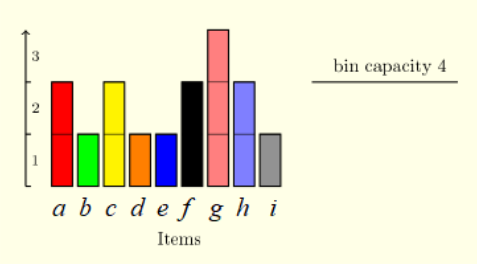
\includegraphics[width=6cm]{images/grap_BPP.png}
    \caption{Dataset}
    \label{fig:grap_BPP}
\end{figure}

\begin{figure}[H]
    \centering
    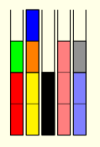
\includegraphics[width=2.5cm]{images/sol1_BPP.png}
    \caption{Prima soluzione candidata del Bin Packing Problem}
    \label{fig:sol1_BPP}
\end{figure}

Consideriamo la prima soluzione proposta, visto che la lista dei prodotti cartesiano
rispetta i due vincoli nella definizione della regione
di fattibilità la soluzione $x'$ è una \textbf{soluzione fattibile}.
$$x'=\left\{(a,1),(b,1),(c,2),(d,2),(e,2),(f,3),(g,4),(h,5),(i,5)\right\}\in X$$
$$f(x')=5$$

\begin{figure}[H]
    \centering
    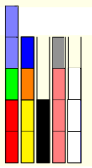
\includegraphics[width=2.5cm]{images/sol2_BPP.png}
    \caption{Seconda soluzione candidata del Bin Packing Problem}
    \label{fig:sol2_BPP}
\end{figure}

Invece, la seconda soluzione proposta è una \textbf{soluzione infattibile}, questo perché gli elementi non stanno
rispettando il secondo vincolo sul volume, e quindi
questo sottoinsieme non è compreso all'interno della regione di fattibilità.
$$x''=\left\{(a,1),(b,1),(c,2),(d,2),(e,2),(f,3),(g,4),(h,1),(i,4)\right\}\notin X$$
$$f(x'')=4$$
Considerando il caso in cui $x''$ fosse una soluzione fattibile avremmo scelto quella tra le soluzioni
proposte, poiché la funzione obiettivo effettua l'ottimizzazione sul minimo.

\subsubsection{Parallel Machine Scheduling Problem (PMSP)}
Il Parallel Machine Scheduling Problem (PMSP), è un problema nel quale un insieme di attività (tasks) deve essere diviso lungo un set di macchine in modo che
il \textit{tempo di completamento} sia minimizzato.

Dati:
\begin{itemize}
    \item Un insieme $T$ di tasks (o \textit{attività}).
    \item Una funzione $d:T \rightarrow \mathbb{N}$ che descrive la lunghezza (temporale) di ogni task.
    \item Un insieme di $M$ macchine.
\end{itemize}

Come prima, il ground set è dato dal prodotto cartesiano di due set forniti:
$$B\equiv T\times M$$
Significa che la soluzione deve essere una coppia $$\langle task,macchina\rangle$$. È importante
sottolineare che la sequenza in cui i task sono eseguiti non è rilevante, invece è rilevante il \textbf{tempo di completamento}
, ovvero il tempo con cui l'ultimo task termina (o il tempo in cui una macchina completa l'esecuzione dei suoi tasks).

La regione di fattibilità include tutte le partizioni delle attività nella macchine:
$$X=\left\{ x\subseteq B : |x\cap B_t|=1 \text{ } \forall t \in T \right\} $$
La \textbf{funzione obiettivo} ha come obiettivo quello di minimizzare il massimo della sommatoria delle lunghezze di tempo per ogni task di ogni macchina:
$$min\underset{x\in X}{f(x)}=max\underset{m\in M}{}\sum_{t:(t,m)\in x} d_t$$

In parole povere, vogliamo trovare il sottoinsieme $x$ che minimizza il tempo di completamento di ciascuna
macchina, dove il tempo di completamento per un singolo task è $\sum_{t:(t,m)\in x} d_t$.
\newline
Per esempio, consideriamo il seguente insieme di dati per tre macchine, $|M|=3$, e sette task differenti $|T|=7$.

\begin{figure}[H]
    \centering
    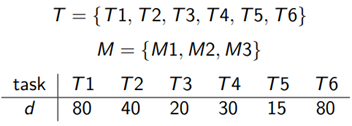
\includegraphics[width=5cm]{images/dataset_PMSP.png}
    \caption{Dataset del Parallel Machine Scheduling Problem}
    \label{fig:dataset_PMSP}
\end{figure}

\begin{figure}[H]
    \centering
    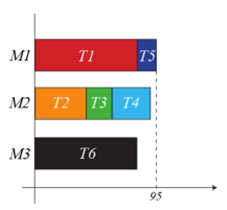
\includegraphics[width=4cm]{images/sol1_PMSP.png}
    \caption{Prima soluzione Parallel Machine Scheduling Problem}
    \label{fig:sol1_PMSP}
\end{figure}

Consideriamo la prima soluzione proposta:
$$x'=\left\{(T1,M1),(T2,M2),(T3,M2),(T4,M2),(T5,M1),(T6,M3)\right\}\in X$$
$$f(x')=95$$
Possiamo notare che questa è una \textbf{soluzione fattibile},
visto che ogni task accade al meno ed al massimo una volta.
Notiamo che il valore assunto dalla funzione obiettivo è $95$, questo proprio
perché l'ultimo task ha un tempo di completamento pari a $95$.

\begin{figure}[H]
    \centering
    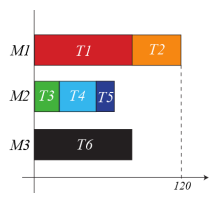
\includegraphics[width=4cm]{images/sol2_PMSP.png}
    \caption{Seconda soluzione Parallel Machine Scheduling Problem}
    \label{fig:sol2_PMSP}
\end{figure}

Consideriamo la seconda soluzione proposta:
$$x''=\left\{(T1,M1),(T2,M1),(T3,M2),(T4,M2),(T5,M2),(T6,M3)\right\}\in X$$
$$f(x'')=120$$
Notiamo che anche questa è una \textbf{soluzione fattibile} visto che ogni task accade al
minimo ed al massimo una volta, in questo casa la funzione obiettivo assume come valore $120$.
Questo significa che fra le due soluzioni proposte la prima è quella \textbf{ottima}.

\subsubsection{Interludio 2: la funzione obiettivo, ancora}
È necessario familiarizzare con il fatto che il ground set $B$ non è sempre uno degli insiemi
forniti nel problema, ma può essere formato dalla combinazione (come il prodotto cartesiano)
di diversi insiemi forniti. Ora affrontiamo la domande proposte nell'ultimo interludio.

\textit{Le funzioni oggettivi di che tipo sono? (additive, quadratiche,...)}
Questa volta le funzioni oggettive per il BPP e PMSP \textbf{non} sono additive, e non sono neanche banali.
È presente un algoritmo polinomiale per calcolare la funzione obiettivo, seppur non complesso,
non è semplice come per i problemi precedenti.

Notiamo che piccole modifiche alle soluzioni hanno un impatto \textit{variabile} sull'obiettivo, per esempio
consideriamo la seconda soluzione $x''$ del PMSP:
\begin{itemize}
    \item Spostare il task $T5$ sulla macchina $M1$, allunga il tempo di completamento complessivo$M1$,
          il risultato della funzione obiettivo cambia perché viene incrementato del task spostato (\textit{\textbf{impatto corrispondente al tempo del task spostato}}).
    \item Spostare il task $T5$ sulla macchina $M3$, non modifica il tempo di completamento complessivo
          delle macchine, il risultato della funzione obiettivo rimane lo stesso (\textit{\textbf{impatto zero}}).
    \item Spostare il task $T2$ sulla macchina $M2$, comporta una modifica dei tempi di completamento
          complessivi, il risultato della funzione obiettivo cambia poiché l'ultimo task viene spostato (\textit{\textbf{impatto intermedio}})

\end{itemize}

In fatti, l'impatto di una modifica di una soluzione dipende :
\begin{itemize}
    \item Da entrambi gli elementi modificati.
    \item E dagli elementi non modificati (questo è contrario alle cose dette nell'interludio 1).
\end{itemize}

Un punto interessante è che la funzione obiettivo del PMSP tende ad essere \textbf{piatta}, ovvero che sono presenti
molteplici soluzioni all'interno del problema dove il valore della funzione rimane lo stesso anche se avvengono
delle modifiche (l'esempio precedente, la soluzione $x''$ rimane fissa per diverse combinazioni su $120$).

\subsection{Problemi delle funzioni logiche}
\subsubsection{The Max-SAT problem}
Il problema del Max-Sat, sia da una formula in \textbf{forma normale congiuntiva}
(CNF, \textit{Conjunctive Normal Form}), si vogliono fornire in ingresso dei valori di
verità alle variabili logiche della CNF tali per cui la formula venga
soddisfatta (valutata come vera).

Dati:
\begin{itemize}
    \item Un insieme $V$ di \textbf{variabili logiche} $x_j$ con valori in $\mathbb{B}\in \{0,1\}$.
    \item Un \textbf{letterale} $l_j(x)\in {x_j,\overline{x}_j}$ che è una funzione che consiste in una variabile logica
          \textit{affermata} o \textit{negata}.
    \item Una \textbf{formula logica} $C_i(x)=l_{i,1} \lor ... \lor l_{i,n_i}$, la quale è
          una disgiunzione o \textit{somma logica} (OR) di letterali. Soddisfare una formula
          logica significa fargli assumere valore 1.
    \item Una formula in \textbf{forma normale congiuntiva} $CNF(x)=C_1\land ... \land C_n$ è una congiunzione di \textit{prodotti logici} di formule logiche.
    \item Una funzione $w$ che provvede dei \textit{pesi} per la formula CNF. La funzione associa ogni formula logica
          della CNF ad un rispettivo peso.
\end{itemize}

Visto che la soluzione consiste in un sottoinsieme caratterizzato dall'assegnamento
di valori di verità a variabili logiche, il \textbf{ground set} sarà il prodotto cartesiano
fra le variabili logiche e l'insieme dei numeri booleani:
$$B=V\times\mathbb{B}=\left\{(x_1,0),(x_1,1),...,(x_n,0),(x_n,1)\right\}$$

La \textbf{regione di fattibilità} è l'insieme delle soluzioni fattibili tali che una \textit{variabile}
venga considerata al più una volta. Essa include tutti sottoinsiemi costituenti
gli assegnamenti semplici che sono:
\begin{itemize}
    \item \textbf{completi}, ovvero che ad ogni variabile corrisponde \textit{almeno} un letterale.
    \item \textbf{consistenti}, ovvero che per ogni variabile corrisponde \textit{al massimo} un letterale.
\end{itemize}

$$X=\left\{x\subseteq B : |x\cap B_v|=1 \text{ }\forall v \in V \right\}$$
$$B_{xj}=\{(x_j,0),(x_j,1)\}$$

La \textbf{funzione obiettivo} (come sempre ottimizzata):
$$max\underset{x\in X}{f(x)}=\sum_{i:C_i(x)=1}w_i$$
L'obiettivo è quello di massimizzare il peso totale della \textit{formula logica soddisfatta}
segnata come $C_i(x)=1 \text{ per } i=1,...,n$ (dove $n$ è il numero di formule logiche presenti).

Consideriamo il seguente esempio:

$$V=\left\{x_1,x_2,x_3,x_4\right\}$$
$$L=\left\{x_1, \overline{x}_1, x_2, \overline{x}_3, x_3,\overline{x}_4, x_4\right\}$$
$$C_1=\overline{x}_1\lor x_2 \text{ ... } C_7=x_2$$
$$CNF = (\overline{x}_1\lor x_2 )\land (\overline{x}_1\lor x_3 )\land (\overline{x}_1\lor \overline{x}_3 )\land (\overline{x}_2\lor x_4 )\land (\overline{x}_2\lor \overline{x}_4 )\land x_1\land x_2$$
$$w_i=1 \forall C_i$$

Consideriamo adesso la seguente soluzione:
$$x=\left\{(x_1,0),(x_2,0),(x_3,1 ),(x_4,1)\right\}$$
La funzione obiettivo per questa soluzione assume valore $f(x)=5$, significa che soddisfa
$5$ formule delle $7$.

\textit{Risulta semplice trovare il valore della funzione obiettivo?} Non proprio, la complessità
della funzione oggettive è polinomiale

In caso di pesi uniformi sono presenti un campo ristretto di valori, che vanno da $0$ a $n$,
il numero di formule logiche, anche se sono presenti $2^|V|$ combinazioni che possono essere considerate.

\subsection{Problemi con matrici numeriche}
\subsubsection{Set covering problem (SCP)}
Data una \textbf{matrice binaria} ed una \textbf{funzione costo} definita per ogni
colonna della matrice (come vettore), si vuole selezionare il sottoinsieme di
colonne che coprono tutte le righe di costo minimo.

Dati:
\begin{itemize}
    \item Matrice binaria $A\in\mathbb{B}^{m,n}$ con insieme delle righe $R$ e insieme delle colonne $C$.
    \item La colonna $j\in C$ copre la riga $i\in R$ quando $a_{ij}=1$.
    \item Una funzione $c:C\rightarrow\mathbb{N}$ provvede il costo di ogni colonna.
\end{itemize}

Il \textbf{ground set} è l'insieme delle colonne.
$$B\equiv C$$
La \textbf{regione di fattibilità} include tutti i sottoinsiemi delle colonne che coprono
tutte le righe.
$$X=\left\{x\subseteq B : \sum_{j\in x}a_{ij}\geq 1 \text{ }\forall i \in R\right\}$$

L'obiettivo è \textit{minimizzare} il costo totale delle colonne selezionate, la \textbf{funzione obiettivo}
è additiva, molto veloce da calcolare ed aggiornare, però la \textit{fattibilità} non è
semplice da ottenere.
$$min\underset{x\in X}{f(x)}=\sum_{j\in x}c_j$$

Consideriamo il seguente esempio di una matrice con il relativo vettore dei costi:

\begin{figure}[H]
    \centering
    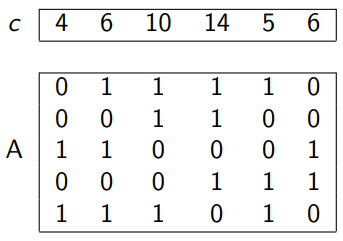
\includegraphics[width=5cm]{images/SCP_datasets.png}
    \caption{Dataset del Set Covering Problem (SCP)}
    \label{fig:dataset_SCP}
\end{figure}
Notiamo che la terza e la quinta riga (iniziando dall'alto) sono coperte dalla prima
colonna. Infatti, \textit{"set covering"}, si coprono i \textit{set} (righe) con
\textit{subset} (colonne).

Consideriamo adesso una prima soluzione proposta:
\begin{figure}[H]
    \centering
    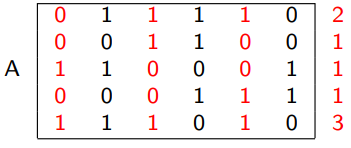
\includegraphics[width=5cm]{images/SCP_first_sol.png}
    \caption{Prima soluzione proposta del SCP}
    \label{fig:sol1_SCP}
\end{figure}

$$x'={c_1,c_2,c_5 }\in X$$
$$f(x')=19$$
La prima soluzione $x'$ è una \textbf{soluzione fattibile}, perché ogni riga ha almeno un elemento
$a_{ij}\geq 1$.

\begin{figure}[H]
    \centering
    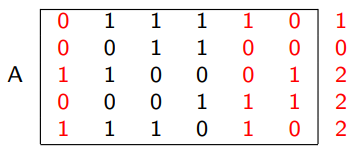
\includegraphics[width=5cm]{images/SCP_snd_sol.png}
    \caption{Seconda soluzione proposta del SCP}
    \label{fig:sol2_SCP}
\end{figure}

$$x''={c_1,c_5,c_6 }\notin X$$
$$f(x'')=15$$

La seconda soluzione $x''$ \textbf{non è una soluzione fattibile}, dato che la Seconda
riga non è coperta da almeno un elemento delle colonne. Comunque, nel caso in cui
la seconda soluzione sia una soluzione fattibile, allora quest'ultima sarebbe una
soluzione migliore della prima.

\subsubsection{Interludio 3: il test di fattibilità}
Solitamente, gli algoritmi euristici \textbf{richiedono} di risolvere il seguente
problema: \textit{Dato un sottoinsieme $x$, è fattibile o infattibile?}, in breve
$x\in X \text{?}$. Come risolvere questo problema? Innanzitutto, è un \textbf{problema di decisione}.

Consideriamo SCP, la fattibilità può essere decisa passando per ogni riga e sommando gli $1$ che appaiono
nella colonna selezionata: se una qualsiasi riga ha una somma complessiva pari a $0$ la soluzione sarà
\textbf{infattibile}.

Nel caso del KP, il test di fattibilità richiede di calcolare dalla soluzione e testare un singolo numero
(il peso totale rispetto alla capacità dello zaino) proprio come nel MDP, dove la cardinalità della soluzione
si trovava sotto una restrizione $k$.

Altri problemi come il Max-SAT ed il PMSP richiedono di testare la fattibilità su un singolo insieme di
numeri (numero di variabili logiche non si ripeta nella soluzione $x\cap B_v$), mentre problemi come il BPP richiedono di testare su diversi insiemi di numeri (i volumi degli oggetti rispetto
alla capacità dei container).

Alcune modifiche alle soluzioni vengono vietate \textit{a priori} per evitare l'inammissibilità delle soluzioni.
Supponiamo di avere una soluzione fattibile per il MDP, una qualsiasi modifica in cui il numero di punti non è uguale
al numero di punti aggiunti rende la soluzione \textbf{infattibile}.

Alcune modifiche non garantiscono \textbf{inammissibilità} (unfeasible) della soluzione, le quali richiedono un test
\textit{a posteriori} come nel PMSP.

\subsection{Set Packing Problem}
Il Set Packing Problem è un problema molto simile al precedente SCP, questo perché appartiene alla stessa
classe di problemi e provvede un valore per ogni colonna.


Dati:
\begin{itemize}
    \item Una \textbf{matrice binaria} $A\in \mathbb{B}^{m,n}$ con insieme delle righe $R$ e insieme delle colonne $C$.
    \item Sia definito un conflitto tra due colonne $j',j'' \in C$ quando $a_{ij'}=a_{ij''}=1$.
    \item Una funzione $\phi:C\rightarrow \mathbb{N}$ che provvede il valore di ogni colonna.
\end{itemize}
Il \textbf{ground set} è ancora l'insieme delle colonne:
$$B\equiv C$$
La \textbf{regione di fattibilità} include tutti i sottoinsieme di colonne che non sono in conflitto:
$$X=\left\{x\subseteq B:\sum_{j\in x}a_{ij}\leq 1 \text{ } \forall i \in R\right\}$$

L'obiettivo consiste nello scegliere le colonne di valore massimo senza che siano presenti \textit{conflitti}.
$$max\underset{x\in X}{f(x)}=\sum_{j \in x}\phi_j$$

Prendiamo in considerazione la seguente matrice:

\begin{figure}[H]
    \centering
    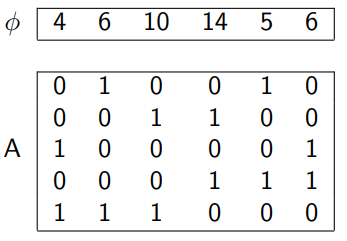
\includegraphics[width=5cm]{images/SPP_dataset.png}
    \caption{Dataset Set Packing Problem}
    \label{fig:datasets_SPP}
\end{figure}

\begin{figure}[H]
    \centering
    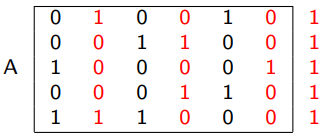
\includegraphics[width=5cm]{images/SPP_first_sol.png}
    \caption{Prima soluzione proposta del SPP (\textit{Set Packing Problem})}
    \label{fig:fst_sol_SPP}
\end{figure}


La prima soluzione proposta è $x'=\left\{c_2,c_4\right\}\in X$, con valutazione della funzione obiettivo
$f(x')=20$. Questa è una soluzione \textbf{fattibile}, visto che non presenti conflitti sulle righe delle colonne
selezionate.

\begin{figure}[H]
    \centering
    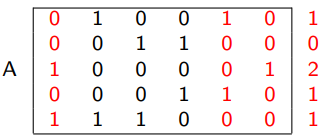
\includegraphics[width=5cm]{images/SPP_snd_sol.png}
    \caption{Seconda soluzione proposta del SPP (\textit{Set Packing Problem})}
    \label{fig:snd_sol_SPP}
\end{figure}
In questo caso \textbf{non è una soluzione fattibile}, visto che avviene il conflitto sulla terza riga, anche quando
la valutazione della funzione obiettivo era meglio della prima soluzione, le somme valutate non sono ottenute dalla
regione di fattibilità $X$.

\subsection{Set Partitioning Problem}
Il problema di Set Partitioning (non lo chiameremo con l'acronimo inglese), è una fusione dei due precedenti problemi
SCP e SPP.

Dati:
\begin{itemize}
    \item Una \textbf{matrice binaria} $A\in \mathbb{B}^{m,n}$ con insieme delle righe $R$ e insieme delle colonne
          $C$.
    \item Una funzione $c:C\rightarrow\mathbb{N}$ che fornisce il costo di ogni colonna.
\end{itemize}
La risoluzione del problema prevede di selezionare il sottoinsieme di \textit{costo minimo} delle colonne
che non sono in conflitto.
Il \textbf{ground set}, anche questa volta, è l'insieme delle colonne:
$$B\equiv C$$
La \textbf{regione di fattibilità} include tutti i sottoinsiemi di colonne che coprono tutte le righe che non
sono in conflitto:
$$X=\left\{x\subseteq C:\sum_{j\in x}a_{ij}=1 \text{ }\forall i \in R\right\}$$
$$min\underset{x\in X}{f(x)}=\sum_{j\in x}c_j$$

Consideriamo la seguente matrice binaria:

\begin{figure}[H]
    \centering
    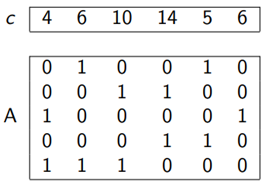
\includegraphics[width=5cm]{images/SPP2_dataset.png}
    \caption{Dataset del Set Partitioning Problem}
    \label{fig:dataset_SPP2}
\end{figure}

Ora prendiamo in considerazione la prima soluzione proposta:

\begin{figure}[H]
    \centering
    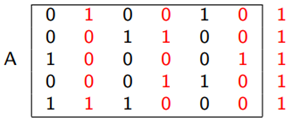
\includegraphics[width=5cm]{images/SPP2_fst_sol.png}
    \caption{Prima soluzione del SPP (\textit{Set Partitioning Problem})}
    \label{fig:fst_sol_SPP2}
\end{figure}

$$x'=\left\{c_2,c_3,c_6\right\}\in X$$
$$f(x')=26$$
Notiamo che la soluzione $x'$ è un \textbf{soluzione fattibile}, visto che gli elementi appartenenti alle
selezionati si trovano colonne si trovano in una maniera da non generare conflitti lungo le righe (la sommatoria
degli elementi lungo le righe non porta ad un risultato diverso da $1$).

Ora consideriamo la seconda soluzione candidata:
\begin{figure}[H]
    \centering
    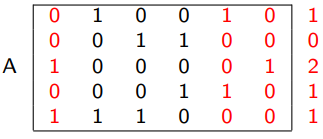
\includegraphics[width=5cm]{images/SPP2_snd_sol.png}
    \caption{Seconda soluzione del SPP (\textit{Set Partitioning Problem})}
    \label{fig:snd_sol_SPP2}
\end{figure}

$$x''=\left\{c_1,c_5,c_6\right\}\notin X$$
$$f(x'')=15$$

Anche se il risultato della funzione obiettivo ha un valore migliore (più piccolo) rispetto a quello della
prima soluzione, la soluzione $x''$ \textbf{non è una soluzione fattibile}. Questo perché, gli elementi sulla terza
riga si trovano in conflitto ($\sum_{j\in x}a_{ij}\geq 1$), ed anche perché la seconda riga non viene \textit{coperta}
da alcuna colonna ($\sum_{j\in x}a_{ij}=0$).

\subsection{Interludio 4: ricerca di soluzioni fattibili}
Gli algoritmi euristici spesso richiedono di risolvere un altro problema: \textit{trovare una soluzione
    che fattibile $x\in X$}, questo è un \textbf{problema di ricerca}. Chiaramente dato che le soluzioni
sono definite da una soluzione iniziale, le euristiche di scambio e ricombinazione hanno bisogno di
partire da un sottoinsieme valido tale per cui esso stesso sia una soluzione fattibile.

In base al problema la soluzione può essere banale:
\begin{itemize}
    \item Alcuni insiemi sono sempre fattibili: $x=\emptyset$ (come nel KP, SPP) o $x=B$ (nel SCP).
    \item Alcune soluzioni casuali soddisfano un vincolo come $|x|=k$ (nel MDP).
    \item Alcune soluzioni casuali soddisfano vincoli consistenti, come assegnare un task per ogni macchina
          come nel PMSP, o un valore ad ogni variabile logica come nel Max-SAT.
\end{itemize}
Oppure può essere difficile:
\begin{itemize}
    \item Nel BPP il numero di container deve essere sufficientemente grande.
    \item Nel SPP non è conosciuto alcun algoritmo polinomiale per risolvere il problema.
\end{itemize}

Alcuni algoritmi ingrandiscono al regione di fattibilità da $X$ a $X'$ (processo detto \textit{"rilassamento"}),
la funzione obiettivo $f$ deve essere estesa anch'essa da $X$ a $X'$, ma spesso $X'\setminus X$ provvede delle
soluzioni migliori.

\subsection{Problemi sui grafi}
\subsubsection{Vertex Cover Problem}
Dato un grafo indiretto $G=(V,E)$, selezionare un sottoinsieme di vertici di cardinalità minima tale che ogni
arco del grafo sia incidente a quest'ultimo.

Il \textbf{ground set} è l'insieme dei vertici:
$$B\equiv V$$
La \textbf{regione di fattibilità} include tutti i sottoinsiemi dei vertici tali che gli archi del grafo siano
incidenti ad essi:
$$X=\left\{x\subseteq V:x\cap (i,j)\neq\emptyset \text{ }\forall (i,j)\in E\right\}$$
L'obiettivo è minimizzare il numero di vertici selezionati:
$$min\underset{x\in X}{f(x)}=|x|$$

\begin{figure}[H]
    \centering
    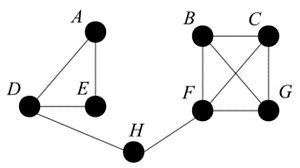
\includegraphics[width=5cm]{images/VCP_dataset.png}
    \caption{Dataset del Vertex Covering Problem}
    \label{fig:dataset_VCP}
\end{figure}

Prima soluzione proposta:
\begin{figure}[H]
    \centering
    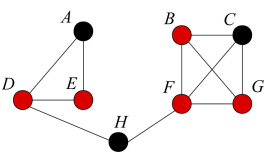
\includegraphics[width=5cm]{images/VCP_sol1.png}
    \caption{Prima soluzione proposta per il VCP}
    \label{fig:fst_sol_VCP}
\end{figure}

$$x'=\left\{ B,D,E,F,G \right\} \in X$$
$$f(x')=5$$
Notiamo che $x'$ è una \textbf{soluzione fattibile}, questo perché il sottoinsieme di vertici selezionato interseca
ogni arco del grafo (appartiene alla regione di fattibilità).

Guardiamo la seconda soluzione proposta:
\begin{figure}[H]
    \centering
    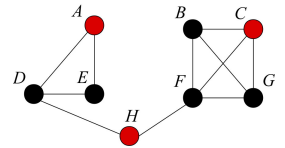
\includegraphics[width=5cm]{images/VCP_sol2.png}
    \caption{Seconda soluzione proposta per il VCP}
    \label{fig:snd_sol_VCP}
\end{figure}

Invece, la seconda soluzione \textbf{non è una soluzione fattibile}, anche se la funzione obiettivo porta ad un
risultato che è più convincente della soluzione precedente, questo sottoinsieme non appartiene alla regione di
fattibilità (il sottoinsieme di vertici selezionato non è incidente a tutti gli archi del grafo, e.g.: $(d,e)$).

\subsubsection{Maximum Clique Problem (MCP)}
Dati:
\begin{itemize}
    \item Un \textbf{grafo indiretto} $G=(V,E)$.
    \item Una funzione $w:V\rightarrow \mathbb{N}$ che provvede il peso di ogni vertice.
\end{itemize}
Selezionare il sottoinsieme di coppie di vertici adiacenti di peso massimo. Il \textbf{ground set} è l'insieme
dei vertici.
$$B\equiv V$$

La \textbf{regione di fattibilità} include tutti i sottoinsiemi di coppie di vertici adiacenti.
$$X=\left\{x\subseteq V:(i,v)\in E \text{ }\forall i \in x, \forall j \in x \setminus \{i\}\right\}$$
L'obiettivo è quello di massimizzare il peso dei vertici selezionati:
$$f(x)=\sum_{j\in x}w_j$$

Consideriamo il seguente grafo indiretto costituito da \textbf{pesi uniform} $w_i=1 \forall i\in V$.
\begin{figure}[H]
    \centering
    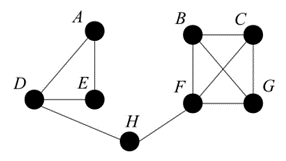
\includegraphics[width=5cm]{images/MCP_dataset.png}
    \caption{Dataset per il Maximum Clique Problem}
    \label{fig:MCP_dataset}
\end{figure}
Consideriamo la prima soluzione proposta:
\begin{figure}[H]
    \centering
    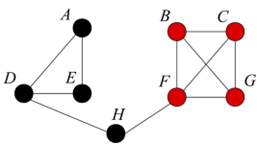
\includegraphics[width=5cm]{images/MCP_sol1.png}
    \caption{Prima soluzione proposta per il MCP}
    \label{fig:MCP_sol1}
\end{figure}
$$x'=\left\{B,C,F,G\right\}\in X$$
$$f(x')=4$$
La prima soluzione proposta è una soluzione \textbf{fattibile}, visto che ogni coppia nel sottoinsieme di vertici
presenta un arco tra di loro.
\begin{figure}[H]
    \centering
    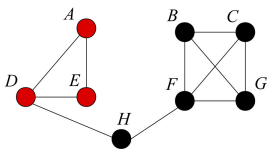
\includegraphics[width=5cm]{images/MCP_sol2.png}
    \caption{Seconda soluzione proposta per il MCP}
    \label{fig:MCP_sol2}
\end{figure}

$$x'=\left\{A,D,E\right\}\in X$$
$$f(x')=3$$
La seconda soluzione proposta è anch'essa una soluzione \textbf{fattibile}, per lo stesso motivo precedente.

\subsubsection{Maximum Independent Set}
Questo problema è opposto al MCP, vogliamo trovare un sottoinsieme di vertici di peso massimo che non è
connesso da archi.
Dati:
\begin{itemize}
    \item Un \textbf{grafo indiretto} $G=(V,E)$.
    \item Una funzione $w:V\rightarrow \mathbb{N}$ che provvede un peso per ogni arco.
\end{itemize}
Il \textbf{ground set} è l'insieme dei vertici.
$$B\equiv V$$
La \textbf{regione di fattibilità} include tutti i sottoinsiemi di vertici i cui archi \textit{non sono adiacenti}.
$$X=\left\{x\subseteq B : (i,j) \notin E \text{ }\forall i \in x, \forall j \in x\setminus \{i\}\right\}$$
L'obiettivo è quello di massimizzare il peso dei vertici selezionati.
$$max\underset{x\in X}{f(x)}=\sum_{j\in x}w_j$$
Consideriamo il seguente grafo indiretto con \textit{pesi uniformi}.
\begin{figure}[H]
    \centering
    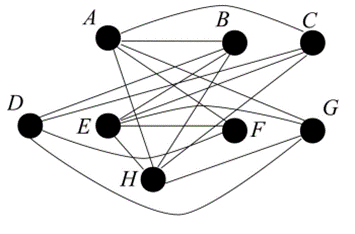
\includegraphics[width=5cm]{images/MIS_dataset.png}
    \caption{Dataset per il Maximum Independent Set}
    \label{fig:MIS_dataset}
\end{figure}
Adesso consideriamo la prima soluzione proposta:
\begin{figure}[H]
    \centering
    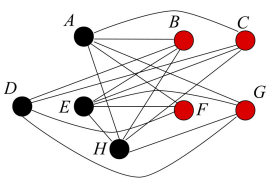
\includegraphics[width=5cm]{images/MIS_sol1.png}
    \caption{Prima soluzione per il MIS}
    \label{fig:MIS_1}
\end{figure}

$$x'=\left\{B,C,F,G\right\}\in X$$
$$f(x')=4$$
La soluzione $x'$ è una soluzione \textbf{fattibile}, ogni vertice del sottoinsieme proposto \textit{non è connesso}
con un altro vertice dello stesso sottoinsieme.

Consideriamo adesso una seconda proposta:
\begin{figure}[H]
    \centering
    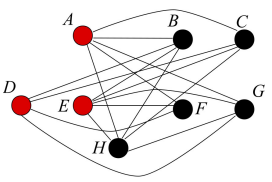
\includegraphics[width=5cm]{images/MIS_sol2.png}
    \caption{Seconda soluzione per il MIS}
    \label{fig:MIS_2}
\end{figure}

$$x''=\left\{A,D,E\right\}\in X$$
$$f(x'')=3$$
Anche la seconda soluzione è una \textbf{soluzione fattibile}.

\subsubsection{Interludio 5: le relazioni tra i problemi}
Come al solito le domande che uno si dovrebbe porre per un qualsiasi problema sono le solite :
\begin{itemize}
    \item \textit{Come si calcola la funzione obiettivo?}
    \item \textit{Cosa succede se togliamo un vertice?}
    \item \textit{Come si verifica la fattibilità?}
    \item \textit{Cosa succede se aggiungiamo o rimuoviamo un vertice ad una soluzione fattibile?}
\end{itemize}

Questi ultimi tre problemi sui grafi che abbiamo affrontato erano molto simili. Dovrebbe essere già noto
dalla \textbf{teoria delle complessità computazionali} che alcuni problemi possono essere \textbf{ridotti} ad altri
problemi, e che si possa \textit{utilizzare} un problema per risolverne un altro.

Un chiaro esempio è il seguente:
\begin{itemize}
    \item Si parte dall'istanza iniziale del MCP, con un grafo $G=(V,E)$.
    \item Si costruisce il \textbf{grafo complementare} $\overline{G}=(V,(V\times V)\setminus E)$ (un grafo tale
          per cui i vertici adiacenti nel grafo originario ora non lo sono più e viceversa).
    \item Si cerca una soluzione ottima per il MISP su $\overline{G}$.
    \item I vertici corrispondenti danno una soluzione ottimale del MCP su $G$.
\end{itemize}

\begin{figure}[H]
    \centering
    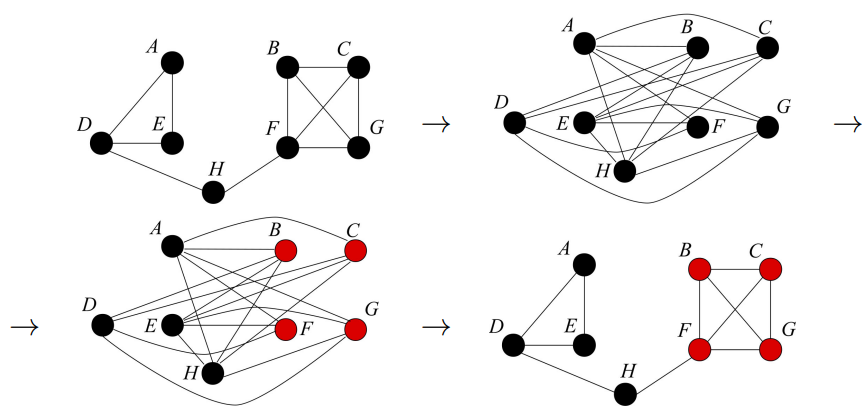
\includegraphics[width=10cm]{images/interlude5_complementary.png}
    \caption{Una soluzione euristica MISP che da una soluzione euristica MCP}
    \label{fig:interlude_5_graph}
\end{figure}

Questo processo può essere applicato anche nel verso opposto.

Anche i problemi SCP (\textit{Set Covering Problem}) e VCP (\textit{Vertex Covering Problem}) P hanno una relazione tra di loro, ma in maniera differente; ogni istanza del
VCP può essere trasformata in un istanza del SCP.
\begin{itemize}
    \item Ogni arco $i$ corrisponde ad una riga della matrice $A$.
    \item Ogni vertice $j$ corrisponde ad una colonna $A$.
    \item Se l'arco $i$ tocca il vertice $j$, l'insieme $a_{ij}=1$, altrimenti $a_{ij}=0$.
    \item Una soluzione ottimale del SCP da una soluzione ottimale del VCP.
\end{itemize}

\begin{figure}[H]
    \centering
    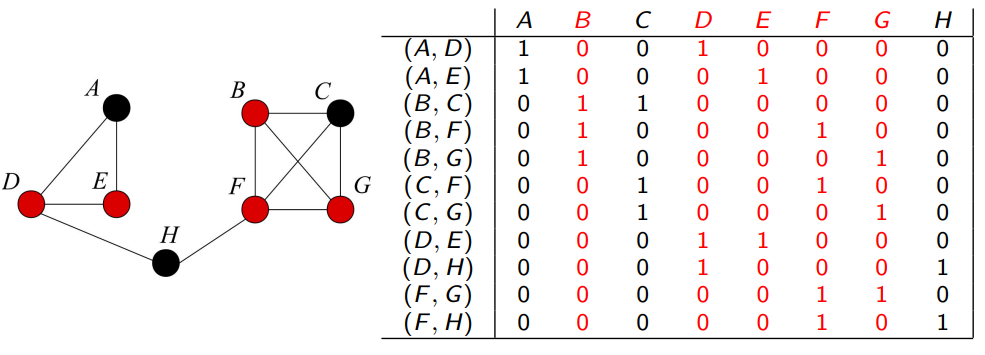
\includegraphics[width=10cm]{images/interlude5_vcp_scp.png}
    \caption{Una soluzione euristica SCP che da una soluzione euristica VCP}
    \label{fig:interlude5_vcp_scp}
\end{figure}
In questo caso non è semplice effettuare il procedimento inverso.

I problemi BPP (\textit{Bin Packing Problem}) e PMSP (\textit{Parallel Machine Scheduling Problem})
sono equivalenti, ma in una maniera più sofisticata:
\begin{itemize}
    \item I task corrispondono a gli oggetti.
    \item Le macchine corrispondono ai container, ma ricordiamo che il BPP cerca di ottimizzare il numero di
          container (data una capacità), mentre il PMSP dato un numero di macchine cerca di ottimizzare il \textit{tempo
              di completamento}.
\end{itemize}

Partiamo da un istanza del BPP:
\begin{itemize}
    \item Facciamo un assunzione sul numero di container ottimali, per esempio $3$.
    \item Costruiamo una corrispondente istanza nel PMSP.
    \item Calcoliamo il tempo di completamento ottimale, per esempio $95$; se eccede la capacità,
          incrementa l'assunzione fatta precedentemente (tipo $4$ o $5$). Nel caso contrario, decrementa
          l'assunzione fatta ($2$ o $1$).
\end{itemize}

\begin{figure}[H]
    \centering
    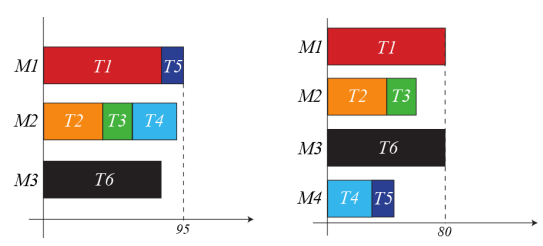
\includegraphics[width=10cm]{images/interlude5_BPP_scp.png}
    \caption{Una soluzione euristica PMSP che da una soluzione euristica BPP}
    \label{fig:interlude5_PMSP_BPP}
\end{figure}
Il processo inverso è possibile. I due problemi sono equivalenti, ma ognuno dei due deve venire risolto molteplici
volte.

È importante sottolineare il fatto che in caso di \textbf{riducibilità}, una soluzione euristica all'interno di un
istanza ridotta è una soluzione euristica per il problema originale; studiare le relazioni tra i problemi è importante
anche senza pensare agli algoritmi.

\subsubsection{Travelling Salesman Problem (TSP)}
Dato:
\begin{itemize}
    \item Un grafo \textbf{diretto} $G=(N,A)$
    \item Una funzione $c:A\rightarrow\mathbb{N}$ che provvede i costi per ogni arco.
\end{itemize}
Si vuole selezionare un ciclo di costo minimo che visiti tutti i nodi del grafo. Il \textbf{ground set} è l'insieme
degli archi.
$$B\equiv A$$
La \textbf{regione di fattibilità} include i cicli che visitano tutti i nodi del grafo (\textbf{cicli Hamiltoniani}).

L'obiettivo è minimizzare il costo totale degli archi selezionati.
$$min\underset{x\in X}{f(x)}=\sum_{j\in x}c_j$$

\textit{Come determinare quando un sottoinsieme è una soluzione fattibile?} Quel sottoinsieme deve identificare
un ciclo sul grafo ed ogni nodo deve avere esattamente un arco entrante ed uno uscente (ma sempre facente parte
del sottoinsieme). Inoltre, una visita del grafo utilizzando gli archi del sottoinsieme dovrebbe visitare tutti i
nodi, in altre parole non sono previste sotto visite di $G$.

\textit{Cosa accade se si effettua una modifica di una soluzione fattibile?} Questo dipende dal tipo della modifica
effettuata sulla soluzione, potrebbe essere necessario ricalcolare la funzione obiettivo.

\textit{Risulta difficile trovare una soluzione fattibile?} Trovare una soluzione che sia fattibile
potrebbe essere altrettanto difficile; in generale un grafo Hamiltoniano (ovvero che presenta un
ciclo Hamiltoniano) è un problema NP-completo, è di risoluzione banale solo nei grafi \textbf{completi}.

Consideriamo il seguente grafo diretto e pesato:
\begin{figure}[H]
    \centering
    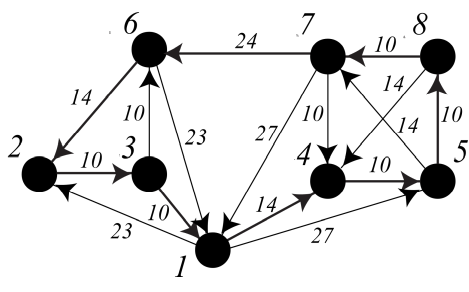
\includegraphics[width=7cm]{images/TSP_dataset.png}
    \caption{Dataset per il Travelling Salesman Problem}
    \label{fig:tsp_dataset}
\end{figure}

Consideriamo la prima soluzione proposta:
\begin{figure}[H]
    \centering
    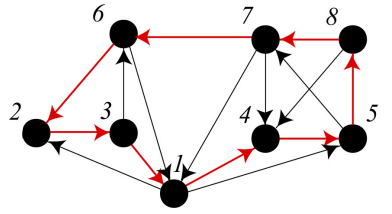
\includegraphics[width=7cm]{images/TSP_sol1.png}
    \caption{Prima soluzione del TSP}
    \label{fig:tsp_1_sol}
\end{figure}

$$x'=\left\{(1,4),(4,5),(5,8),(8,7),(7,6),(6,2),(2,3),(3,1)\right\}\in X$$
$$f(x')=102$$
La soluzione $x'$ è una soluzione \textbf{fattibile}.

Consideriamo la seconda soluzione proposta:
\begin{figure}[H]
    \centering
    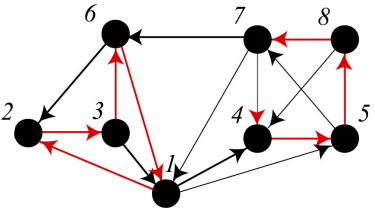
\includegraphics[width=7cm]{images/TSP_sol2.png}
    \caption{Seconda soluzione del TSP}
    \label{fig:tsp_2_sol}
\end{figure}
$$x''=\left\{(4,5),(5,8),(8,7),(7,4),(1,2),(2,3),(3,6),(6,1)\right\}\notin X$$
$$f(x'')=106$$
La soluzione $x''$ è una soluzione \textbf{fattibile}.

\subsubsection{Minimum Capacitated Spanning Tree Problem (MCSTP)}
Dati:
\begin{itemize}
    \item Un grafo indiretto $G=(V,E)$ con un vertice radice $r\in V$
    \item Una funzione $c:E\rightarrow \mathbb{N}$ che provvede il \textit{costo} di ogni arco.
    \item Una funzione $w:V\rightarrow \mathbb{N}$ che provvede il peso di ogni vertice.
    \item Un numero $W\in \mathbb{N}$ che è la capacità di ogni sotto albero.
\end{itemize}

Si vuole selezionare un \textbf{minimo albero ricoprente} tale che ogni ramo (sotto albero rispetto alla radice)
rispetti la capacità massima $W$. Il \textbf{ground set} è l'insieme degli archi.

$$B\equiv E$$

La \textbf{regione di fattibilità} include tutti gli alberi ricoprenti tali che il peso costituito dai vertici
rispetti la capacità $W$.
L'obiettivo è quello di minimizzare il costo totale degli archi selezionati.

$$min\underset{x\in X}{f(x)}=\sum_{j\in x}c_j$$

Consideriamo il seguente grafo indiretto di pesi uniformi $w_i=1 \forall i\in V$, e con una capacità massima
dei sotto alberi $W=3$.
\begin{figure}[H]
    \centering
    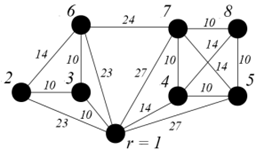
\includegraphics[width=5cm]{images/MCSTP_dataset.png}
    \caption{Dataset del Minimum Capacitated Spanning Tree Problem}
    \label{fig:dataset_MCSTP}
\end{figure}

La prima soluzione candidata:

\begin{figure}[H]
    \centering
    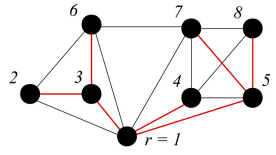
\includegraphics[width=5cm]{images/MCSTP_fst_sol.png}
    \caption{Prima soluzione del MCSTP}
    \label{fig:fst_sol_MCSTP}
\end{figure}

$$x'=\left\{(r,3),(3,2),(3,6),(r,4),(r,5),(5,7),(5,8)\right\}\in X$$
$$f(x')=95$$
Questa è una soluzione \textbf{fattibile}, visto che ogni sotto albero non eccede la
capacità $W$ e i sottoinsiemi sono un minimo albero ricoprente del grafo.

La seconda soluzione candidata:

\begin{figure}[H]
    \centering
    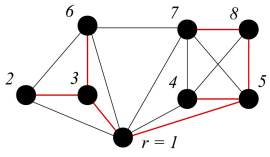
\includegraphics[width=5cm]{images/MCSTP_snd_sol.png}
    \caption{Seconda soluzione del MCSTP}
    \label{fig:snd_sol_MCSTP}
\end{figure}

$$x''=\left\{(r,3),(3,2),(3,6),(r,4),(r,5),(5,7),(5,8)\right\}\notin X$$
$$f(x'')=87$$
Questa \textbf{non è} una soluzione fattibile, visto che il sotto albero destro non rispetta
la capacità massima (nonostante il sottoinsieme sia un albero ricoprente).

Il costo delle operazioni principali cambia, il testi di fattibilità richiede solamente la somma
dei pesi, calcolare la funzione obiettivo richiede risolvere un problema
MST (\textit{Minimum Spanning Tree}).

La funzione obiettivo risulta:
\begin{itemize}
    \item \textbf{Lenta da valutare}, calcolare un MST per ogni sottoinsieme.
    \item \textbf{Lenta da aggiornare}, ricalcolare un MST per ogni sottoinsieme modificato.
\end{itemize}
Se il grafo è \textbf{completo}, i test di ammissibilità sono:
\begin{itemize}
    \item \textbf{Veloci da eseguire}, sommare i pesi dei vertici per ogni sotto albero.
    \item \textbf{Veloci da aggiornare}, sommare i pesi aggiunti e sottrarre quelli rimossi.
\end{itemize}
Visto che la funzione obiettivo è \textbf{additiva}, è abbastanza semplice da valutare, ma mentre
è semplice da ricalcolare, è più difficile verificarne la fattibilità, eccetto per situazioni banali.

Trovare uno \textbf{albero ricoprente capacitato} è un problema fortemente NP-completo, quindi spesso
è difficile trovare una soluzione fattibile a meno che il grafo sia completo. Dato un insieme di vertici,
in ordine si controlla se la soluzione è una soluzione fattibile o meno, è necessario costruire
la corretta rappresentazione dell'albero e poi visitare il sotto albero, sommare i pesi dei vertici, in
una maniera simile ad una visita DFS. \paragraph{Descrizione alternativa}
%Va scritta la descrizione alternativa (secondo o terzo pacco di slide)

\subsubsection{Vehicle Routing Problem (VRP)}
\subsubsection{Interludio 6: combinare rappresentazioni alternative}
Il CMSTP ed il VRP condividono una complicazione interessante: differenti definizioni del
ground set $B$ sono possibili e naturali.
\begin{itemize}
    \item La descrizione come insieme di archi sembra preferibile per gestire la funzione obiettivo.
    \item La descrizione che utilizza un insieme di coppie del tipo
          \newline$(vertice, albero)/(nodo/ciclo)$ sembra migliore per generare
          soluzioni ottime ed ha a che fare con la fattibilità.
\end{itemize}

\noindent\textit{Quale descrizione dovrebbe essere adottata?} Quella che rende più semplice le operazioni più frequenti, oppure una possibilità risulta
quella di utilizzare entrambe le rappresentazioni se le operazioni sono usate molto più frequentemente
che quanto sono aggiornate, in maniera che il fardello di mantenerle aggiornate e consistenti sia accettabile.

Per riassumere, le domande che ci si deve chiedere a riguardo di un problema sono:

\begin{itemize}
    \item Come si calcola la funzione obiettivo?
    \item Come provo che un sottoinsieme sia fattibile?
    \item Come trovo una soluzione fattibile?
    \item Come valutare il test di fattibilità?
    \item Cosa succede quando un cambiamento alla soluzione fattibile viene effettuato: è ancora fattibile?
          Sicuramente non lo è più? È necessario rivalutare da capo la funzione obiettivo o c'è una soluzione migliore?
    \item Quale è la definizione corretta di ground set? Sono qui presenti più definizioni possibili?
    \item Sono presenti relazioni tra questo ed un altro problema?
\end{itemize}

\section{Efficienza teorica}
La seconda parte di questo corso è dedicata alle caratteristiche degli algoritmi euristici: abbiamo precedentemente
descritto gli algoritmi euristici come algoritmi che non provvedono sempre soluzioni corrette, ma che sono
caratterizzati da due aspetti:
\begin{itemize}
    \item Costa molto meno degli algoritmi corretti.
    \item \textit{Spesso} restituisce qualcosa che è \textit{vicino} alla soluzione corretta.
\end{itemize}

Considereremo questi due aspetti, \textbf{costi} e \textbf{qualità}, significa la distanza e la probabilità
di ottenere una certa qualità e considereremo essi da due punti di vista:
\begin{itemize}
    \item \textit{Analisi a priori}, basata sulla teoria.
    \item \textit{Analisi a posteriori}, basata sull'evidenza e sui dati empirici ottenuti dall'esecuzione dell'algoritmo
          su dataset appositi per test.
\end{itemize}

\subsection{Problemi}
Informalmente, un problema è una domanda su un sistema costituito da oggetti matematici. La stessa domanda può
essere spesso posta su diversi sistemi simili.
\begin{itemize}
    \item Un istanza $I\in\mathcal{I}$ consiste in ogni specifico sistema riguardante la domanda.
    \item Una soluzione $S\in\mathcal{S}$ è una risposta corrispondente ad una delle istanze.
\end{itemize}

Per esempio: \textit{$n$ è un numero primo?}, questo è un problema con infinite istanze e due soluzioni.
$$\mathcal{I}=\mathbb{N}^+\setminus{\{1\}}\text{ and }\mathbb{S}=\text{\{yes,no\}}$$

Formalmente, un problema è una funzione che relaziona le istanze e le soluzioni:
$$P:\mathcal{I}\rightarrow\mathcal{S}$$
Definire una funzione non significa sapere come calcolarla.

\subsection{Algoritmi}
Un algoritmo è una \textbf{procedura formale}, composta da passi elementari posti in una sequenza finita, ogni
uno è determinato da un input e dai risultati dei passi precedenti.

Un algoritmo per un problema $P$ è un algoritmo tale per cui un input $I\in\mathcal{I}$ restituisce una soluzione
$S_I\in\mathcal{S}$.
$$A:\mathcal{I}\rightarrow\mathcal{S}$$
Un algoritmo definisce una funzione ed il modo per calcolarla, questo può essere:
\begin{itemize}
    \item \textbf{Esatto}, se la funzione associata coincide con il problema.
    \item Altrimenti \textbf{euristico}.
\end{itemize}
Un algoritmo euristico è utile se risulta:
\begin{itemize}
    \item \textbf{Efficiente}, significa che costa molto meno dell'algoritmo esatto.
    \item \textbf{Efficace}, significa che restituisce frequentemente la soluzione \textit{"vicina"} a quella corretta.
\end{itemize}

\subsection{Costi di un algoritmo euristico}
Il costo di un algoritmo (entrambi i tipi) denotano il costo di computazione durante esecuzione:

\begin{itemize}
    \item \textbf{Tempo}, richiesto per terminare la sequenza finita di passi elementari.
    \item \textbf{Spazio}, quello occupato in memoria dai risultati dei passi precedenti.
\end{itemize}

Il costo in tempo viene molto più discusso perché lo spazio è una risorsa rinnovabile, mentre il tempo non lo è.
Utilizzare lo spazio richiede di utilizzare meno tempo possibile, in oltre è tecnicamente più semplice distribuire
l'utilizzo di spazio che quello del tempo. Lo spazio ed il tempo sono parzialmente intercambiabili,
è possibile ridurre il costo di uno incrementando l'utilizzo dell'altro.

\subsubsection{Il tempo}
Il tempo richiesto per risolvere un problema dipende da diversi aspetti:
\begin{itemize}
    \item L'\textbf{istanza} specifica da risolvere.
    \item L'\textbf{algoritmo} utilizzato.
    \item La \textbf{macchina} che sta eseguendo l'algoritmo.
\end{itemize}
La nostra misura di tempo computazionale dovrebbe essere:
\begin{itemize}
    \item \textbf{Sconnessa} dalla tecnologia, che sia la stessa su macchine differenti.
    \item \textbf{Coincisa}, che viene riassunta in una semplice espressione simbolica.
    \item \textbf{Ordinale}, che sia sufficiente per essere comparata con diversi algoritmi.
\end{itemize}
Il tempo computazionale in secondo per ogni istanza viola tutti i requisiti.

\subsubsection{Complessità asintotica nel caso peggiore}
La complessità asintotica di un algoritmo nel \textbf{caso peggiore} provvede una tale misura
attraverso i seguenti passaggi:
\begin{enumerate}
    \item Definire il tempo come un numero $T$ di operazioni elementari eseguite.
    \item Definire la dimensione di un istanza come opportuno valore di $n$.
    \item Trovare il caso peggiore, ovvero il massimo valore di $T$ su tutte le istanze
          di dimensione $n$. $$T(n)=max\underset{I\in\mathcal{I}_n}{T(I)}\text{  ,  }n\in\mathbb{N}$$
          Ora la complessità in tempo è una funzione $T:\mathbb{N}\rightarrow\mathbb{N}$.
    \item Approssimare $T(n)$ da sotto e/o da sopra con una funzione più semplice $f(n)$, questo
          considerando solamente il loro comportamento asintotico (per $n\rightarrow\infty$).
    \item Collezionare le funzioni in \textbf{classi} con la stessa \textit{funzione di approssimazione}.
\end{enumerate}

\subsubsection{\texorpdfstring{Gli spazi funzionali $\Theta$}{Gli spazi funzionali}}
$$T(n) \in \Theta (f (n))$$
Formalmente significa:
$$\exists c_1, c_2 \in \mathbb{R}^+, n_0 \in \mathbb{N} : c_1 f(n) \leq T(n) \leq c_2 f(n)
    \text{  }\forall n\geq n_0$$

Dove $c_1,c_2$ e $n_0$ sono indipendenti da $n$. $T(n)$ è \textit{"racchiusa"} tra
$c_1 f(n)$ e $c_2 f(n)$, per:

\begin{itemize}
    \item Alcuni \textit{"piccoli"} valori di $c_1$.
    \item Alcuni \textit{"grandi"} valori di $c_2$.
    \item Alcuni \textit{"grandi"} valori di $n_0$.
\end{itemize}

\begin{figure}[H]
    \centering
    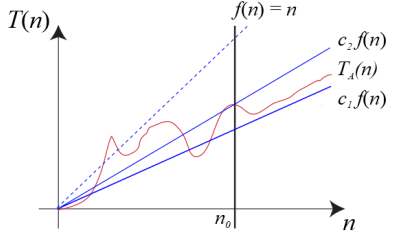
\includegraphics[scale=0.8]{images/theta.png}
    \caption{$f(n)=\Theta(T(n))$}
\end{figure}
Asintoticamente, la funzione $f(n)$ stima la funzione $T(n)$ per un fattore moltiplicativo:
per grandi istanze, il tempo computazionale è al meno ed al più il valore della funzione $f(n)$.

\subsubsection{\texorpdfstring{Gli spazi funzionali $O$}{}}
$$T (n) \in O (f (n))$$
Formalmente significa:
$$\exists c \in \mathbb{R}^+, n_0 \in \mathbb{N} : T(n) \leq c f(n) \text{  }\forall n \geq n_0$$

Dove $c$ e $n_0$ sono indipendenti da $n$. $T(n)$ è \textit{"dominata"} da $c f(n)$, per:
\begin{itemize}
    \item Alcuni \textit{"grandi"} valori di $c$.
    \item Alcuni \textit{"grandi"} valori di $n_0$.
\end{itemize}
Asintoticamente, la funzione $f(n)$ sovrastima la funzione $T(n)$ per un fattore moltiplicativo: per
grandi istanze, il tempo computazionale è al più proporzionale al valore della funzione $f(n)$
\begin{figure}[H]
    \centering
    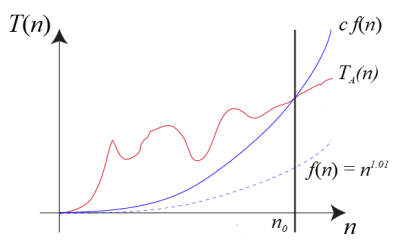
\includegraphics[scale=0.8]{images/ogrande.png}
    \caption{$f(n)=O(T(n))$}
\end{figure}

\subsubsection{\texorpdfstring{Gli spazi funzionali $\Omega$}{}}
$$T (n) \in \Omega (f (n))$$
Formalmente significa:
$$\exists c>0, n_0\in\mathbb{N}:T(n)\geq c f(n) \text{  }\forall n\geq n_0$$
Dove $c$ e $n_0$ sono indipendenti da $n$. $T(n)$ \textit{"domina"} $c f(n)$, per:
\begin{itemize}
    \item Alcuni \textit{"grandi"} valori di $c$.
    \item Alcuni \textit{"grandi"} valori di $n_0$.
\end{itemize}

\begin{figure}[H]
    \centering
    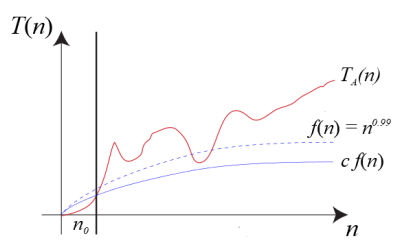
\includegraphics[scale=1]{images/omega.png}
    \caption{$f(n)=\Omega(T(n))$}
\end{figure}

Asintoticamente, $f(n)$ sovrastima $T(n)$ per un fattore moltiplicativo: per alcune grandi istanze,
il tempo computazionale è almeno proporzionale al valore della funzione $f(n)$.

\subsubsection{L'algoritmo esaustivo}
Per i problemi di ottimizzazione combinatoria la dimensione di un istanza può essere misurata
dalla cardinalità del ground set.
$$n=|B|$$

L'\textbf{algoritmo esaustivo}:
\begin{itemize}
    \item Considera ogni sottoinsieme $x\subseteq B$ tale che $x\in 2^{|B|}$.
    \item Testi la fattibilità (se $x\in X$) in un tempo $\alpha(n)$.
    \item In caso positivo, risolve la funzione obiettivo $f(x)$ in tempo $\beta(n)$.
    \item Se necessario, aggiorna il miglior valore trovato finora.
\end{itemize}

La complessità in tempo degli algoritmi esaustivi è :
$$T(n)\in\Theta\left( 2^n\left(\alpha(n)+\beta(n)\right) \right)$$
Questa risulta lo stesso esponenziale, anche se $\alpha(n)$ e $\beta(n)$ sono dei
polinomi (caso più frequente). La maggior parte delle volte l'algoritmo esaustivo
è \textbf{impraticabile}.

\subsubsection{Complessità polinomiale ed esponenziale}
Nei problemi di ottimizzazione combinatoria, la principale distinzione si trova tra:
\begin{itemize}
    \item \textbf{Complessità polinomiale}, $T(n)\in O(n^d)$, dove $d>0$ è costante.
    \item \textbf{Complessità esponenziale}, $T(n)\in\Omega(d^n)$, dove $d>1$ è costante.
\end{itemize}
Nella prima famiglia fanno parte gli \textbf{algoritmi efficienti}, invece nella seconda
quelli \textbf{inefficienti}. In generale, gli algoritmi euristici sono algoritmi polinomiali
per problemi dove l'algoritmo esatto risulta esponenziale.
\subsubsection{Problemi di trasformazione e riduzione}
Una relazione tra problemi permette la progettazione di algoritmi (\textit{interludio 5}).

Progettare un algoritmo per \textbf{trasformazione}:
\begin{enumerate}
    \item Data un istanza di un problema $P$, detta $I_P$, trasformarla in
          una istanza di un altro problema $Q$, $I_Q$.
    \item Data $I_Q$, applicare l'algoritmo $A_Q$ per ottenere la soluzione $S_Q$.
    \item Data $S_Q$, trasformiamola nella soluzione del problema $P$, $S_P$.
\end{enumerate}

Progettare un algoritmo per \textbf{riduzione}:
\begin{enumerate}
    \item Ripetere le trasformazioni $1,2,3$ diverse volte correggendo $I_Q$ basato sulle soluzioni
          $\{S_Q\}$ già ottenute.
\end{enumerate}

I due algoritmi spesso hanno complessità simili: se $A_Q$ è polinomiale (o esponenziale) e:
\begin{itemize}
    \item Costruire $I_Q$ impiegherà tempo polinomiale/esponenziale.
    \item Il numero di iterazioni sarà polinomiale/esponenziale.
    \item Costruire $S_P$ impiegherà tempo polinomiale/esponenziale.
\end{itemize}

Quindi $A_P$ è un algoritmo \textit{polinomiale/esponenziale}.

Il punto è che se si ha una trasformazione nella quale la modifica dell'istanza è
polinomiale, ed il tempo in cui la trasformazione è applicata è polinomiale, allora la
complessità di tutto l'algoritmo dipenderà dalla complessità di $A_Q$.

\subsubitem{Oltre alla complessità del caso peggiore}
La complessità nel caso peggiore ha diversi svantaggi:
\begin{itemize}
    \item Cancella tutte le informazioni delle istanze più semplici, poiché considera
          solamente le istanza con grandi dimensioni.

    \item Fornisce una approssimativa sovrastima del tempo computazionale, che
          in alcuni rari casi è inutile. Per esempio, i problemi di \textit{programmazione
              lineare}, nei quali i problemi hanno infinite soluzioni ma \textit{finite} soluzioni
          base, ed ammettono un algoritmo che ha complessità esponenziale.

          Tuttavia nella maggioranza dei casi gli algoritmi sono polinomi di bassa complessità.
\end{itemize}
\noindent\textit{Cosa se le istanze difficili sono rare nelle applicazioni pratiche?}
Per compensare, uno può investigare:
\begin{itemize}
    \item La \textbf{complessità parametrizzata}, la quale introduce un nuovo rilevante
          parametro $k$ (che è basato sulla dimensione di $n$), ed esprime il tempo come $T(n,k)$.
    \item La \textbf{complessità nel caso medio}, la quale si assume una probabilità di
          distribuzione su $\mathcal{I}$ ed esprime il tempo come il valore atteso.
          $$T(n)=E[T(I)|I\in \mathcal{I}_n]$$

\end{itemize}

\subsection{Complessità parametrizzata}
L'idea è che alcuni algoritmi non sono esponenziali in $n$ ma sono esponenziali in un
altro parametro $k$ che è più piccolo di $n$.

Se entrambi $k$ e $n$ sono grandi, allora ovviamente l'algoritmo è inefficiente, ma se $k$
è piccolo, allora l'algoritmo sarà efficiente e possibilmente anche polinomiale.

Perciò:
\begin{itemize}
    \item Efficiente su istanze con $k$ piccolo.
    \item Inefficiente su istanze con $k$ grande.
\end{itemize}

\begin{figure}[H]
    \centering
    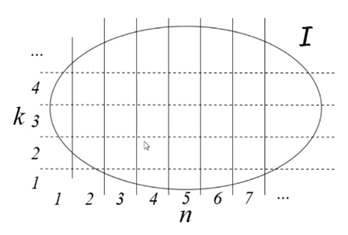
\includegraphics[scale=0.7]{images/param_coplx.png}
    \caption{Insieme delle istanza infinitamente diviso dai parametri $k$ ed $n$}
\end{figure}

Abbiamo tutti gli insiemi delle istanze del nostro problema, possiamo partizionare queste
istanze con un numero infinito di fette per $n$ e per l'altro parametro $k$. Possiamo
considerare il nostro algoritmo.

Il parametro $k$ può fare parte dell'input come la capacità, il massimo numero di
letterali per formula (SAT), il numero di elementi non-zero (problema matrici numeriche),
il massimo grado o il diametro (problemi con i grafi).

Stranamente il parametro aggiuntivo $k$ può essere parte della soluzione (come la \textit{
    cardinalità} nel VCP): in tale caso non puoi conoscere \textit{a priori} se l'algoritmo
è efficiente o meno, ma solo un approssimazione può essere disponibile. Quindi
se $k$ è facente parte della soluzione, solo \textit{a posteriori} sarà possibile
sapere se si tratta di un algoritmo efficiente.

\subsubsection{Bounded tree search (algoritmo con parametro)}
\noindent\textbf{Per esempio, il VCP}
\newline
L'algoritmo esaustivo: per ogni uno dei $2^n$ sottoinsiemi di vertici, testare se
coprono tutti gli archi, calcolare la cardinalità e mantenere il valore più piccolo.
$$T(n,m)\in\Theta(2^n(m+n)),\text{ dove }n=|V|\text{ e }m=|E|$$

Ma se noi già sappiamo una soluzione con $f(x)=|x|=k+1$, possiamo cercare per una soluzione
di $k$ vertici, e progressivamente decrementare $k$ (o ancora meglio utilizzare
la \textbf{ricerca binaria} su $k$).

L'algoritmo naive: per ogni sotto insieme di $k$ vertici, testare se copre tutti gli archi.
$$T(n,m,k)\in\Theta(n^k m)$$
Per una dato $k$ fissato, l'algoritmo risulta di complessità polinomiale. Detto questo
è possibile fare di meglio.\paragraph{Bounded Tree Search per il VCP}, un algoritmo migliore può
essere basato sulla seguente proprietà:
$$x\cap(u,v)\neq\emptyset\text{ }\forall x\in X,(u,v)\in E$$
Ovvero, una qualsiasi soluzione fattibile include almeno un estremo (vertice)
di ogni arco.

Allora l'algoritmo \textbf{Bounded tree search} (\textit{ricerca delimitata da gli alberi}),
vuole trovare $x$ tale che $x\leq k$:
\begin{enumerate}
    \item Scegliere un qualsiasi arco $(u,v)$, sia che $u\in x$ che $u\notin x$ e
          che $v\in x$ (ovvero che uno degli estremi non faccia per forza parte dalla soluzione).
    \item Per ogni caso \textit{"aperto"}, rimuovere i vertici di $x$ e gli archi che
          essi coprono. $$V:=V\setminus x, E:=E\setminus\{e\in E:e\cap x\neq\emptyset\}$$
    \item Se $|x|\leq k$ e $E=\emptyset$, $x$ è la soluzione richiesta.
    \item Se $|x|=k$ e $E\neq\emptyset$, non è presente alcuna soluzione.
    \item Altrimenti ritorna al passo $1$.
\end{enumerate}
La complessità è $T(n,m,k)\in\Theta(2^km)$, polinomiale in $n$ ($m<n^2$). Per $n>>2$,
questo algoritmo è molto più efficiente di quello \textit{naive}.\newline
\noindent\textbf{Esempio del Bounded tree search}
\newline
Nel seguente grafo con $n=10,m=16$, \textit{è presente una soluzione con $|x|\leq 3$?} (quindi
$k=3$).
\begin{figure}[H]
    \centering
    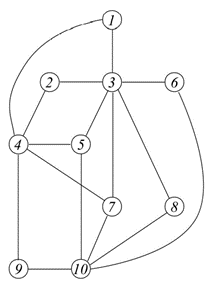
\includegraphics[scale=1]{images/bounded_tree_search_1.png}
    \caption{Stato iniziale del grafo (\textit{Bounded Tree Search})}
\end{figure}
\noindent Algoritmo esaustivo: $\Theta(2^n(m+n))$, con $2^n(m+n)=1024\cdot(16+10)$\newline
Algoritmo naive: $\Theta(n^k m)$, con $n^k m=1000\cdot 16$\newline
Bounded tree search algorithm: $\Theta(2^km)$ con $2^km=8\cdot 16$

\begin{figure}[H]
    \centering
    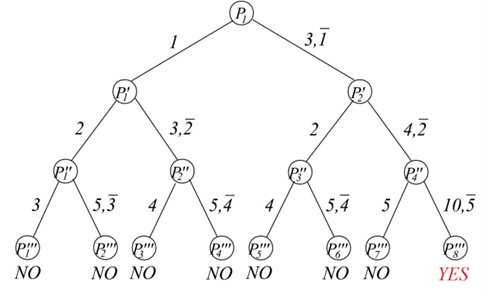
\includegraphics[scale=0.8]{images/bounded_tree_search_2.png}
    \caption{Soluzione del Bounded Tree Search (\textit{ordinamento lessicografico})}
\end{figure}

\subsubsection{Kernelization - "Problem reduction" (algoritmo con parametro)}
La \textit{kernelizzazione} trasforma tutte le istanze di $P$ in istanze più
semplici di $P$, anziché istanze di un altro problema $Q$. Questa pratica è anche
conosciuta con il nome di \textbf{problem reduction} (\textit{riduzione del problema}).

Abbastanza spesso, in fatti, sono presenti delle proprietà molto utili che lo dimostrano:
\begin{itemize}
    \item Esiste una soluzione ottimale che non include certi elementi di $B$ (tali
          elementi possono essere rimossi).
    \item Esiste una soluzione ottimale che include certi elementi di $B$ (tali
          elementi possono essere messi da parte ed aggiunti dopo).
\end{itemize}
In breve rimuove elementi di $B$ senza modificare la soluzione. Possibili risultati
utili sono:
\begin{itemize}
    \item Un algoritmo esatto e polinomiale in $n$ (complessità parametrizzata).
    \item Algoritmi esatti più veloci ed algoritmi euristici.
    \item Migliori soluzioni euristiche.
    \item \textbf{Heuristic kernelization}, applica condizione rilassata sacrificando
          l'ottimalità.
\end{itemize}

\noindent Tornando al problema del VCP, vediamo la \textbf{Kernelization del VCP}:
\newline
Se $\delta_v\geq k+1$, il vertice $v$ appartiene ad una qualsiasi soluzione possibile di
valore $\leq k$. Considerare che $v$ ha $k+1$ archi incidenti e che dovrebbe essere
coperto da altrettanti vertici.
\newline
Algoritmo di kernelizzazione per mantenere solo i vertici della soluzione $x$ con $|x|\leq k$:
\begin{itemize}
    \item Iniziare allo step $t=0$ con $k_0=k$ ed un sottoinsieme di vertici vuoto $x_t:=\emptyset$
    \item Impostare $t=t+1$ ed aggiungere alla soluzione i vertici di grado $\geq k_t+1$.
          $$\delta_v\geq k_t+1\implies x_t := x_{t-1}\cup\{v\}$$
    \item Aggiornare $k_t\text{: } k_t:=k_0-|x_t|$
    \item Rimuovere i vertici con grado zero, quelli di $x$ e degli archi coperti.
          $$V:=\{v\in V : \delta_v > 0\}\setminus x_t$$
          $$E:=\{e\in E : e\cap x_t = \emptyset\}$$
    \item Se $|E|>k_t^2$, non è presente alcuna soluzione fattibile ($k_t$ vertici non sono abbastanza).
    \item Se $|E|\leq k_t^2\implies |V|\leq 2k_t^2$, si applica l'algoritmo esaustivo.
\end{itemize}
La complessità è $T(n,k)\in\Theta(n+m+2^{2k^2}k^2)$.

Per esempio, consideriamo il seguente grafo con $n=10,m=16$, \textit{è presente una
    soluzione con $|x|\leq k_0=5$?}
\begin{figure}[H]
    \centering
    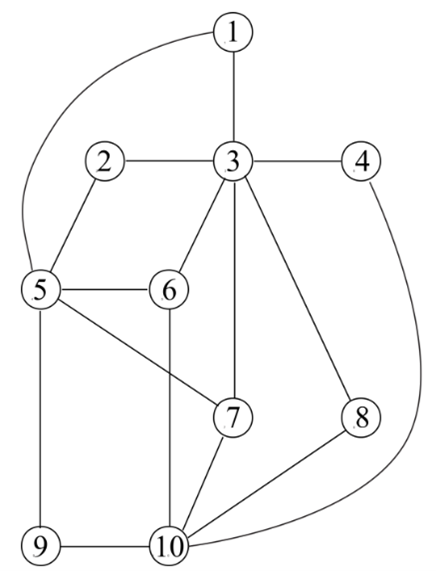
\includegraphics[scale=1]{images/kerneliz_0.png}
    \caption{Grafo d'esempio per la Kernelization del VCP}
\end{figure}

\noindent Algoritmo esaustivo:$\Theta(2^n(m+n))\implies T\approx 2^{10}(10+16)=26624$
\newline
\noindent Algoritmo naive: $\Theta(n^km)\implies T\approx 10^5\cdot 16=16000000$

$\delta_3\geq k_0+1\implies x_1 := \{3\}$ rimozione degli archi incidenti ed avremo $k_1=4$.
\begin{figure}[H]
    \centering
    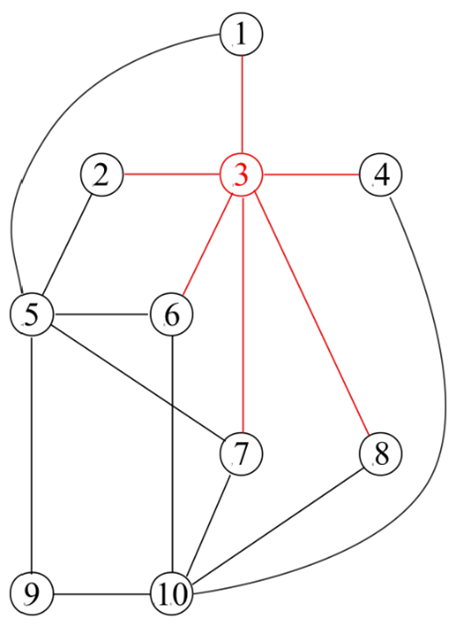
\includegraphics[scale=1]{images/kerneliz_1.png}
    \caption{Rimozione degli archi incidenti con $k_1=4$}
\end{figure}

$\delta_10\geq k_2+1\implies x_3 := \{5,10\}$ rimozione degli archi incidenti ed avremo $k_3=2$.
\begin{figure}[H]
    \centering
    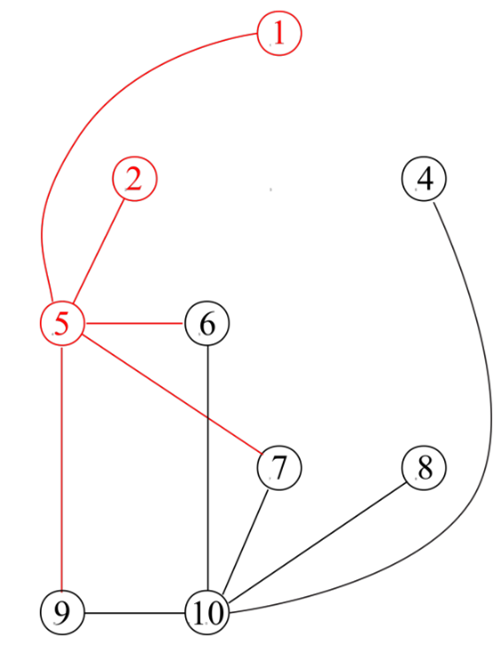
\includegraphics[scale=1]{images/kerneliz_2.png}
    \caption{Rimozione degli archi incidenti con $k_2=3$}
\end{figure}

\begin{figure}[H]
    \centering
    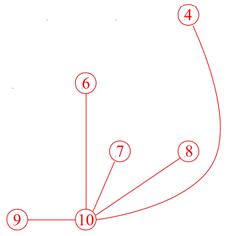
\includegraphics[scale=1]{images/kerneliz_3.png}
    \caption{Rimozione degli archi incidenti con $k_3=2$}
\end{figure}

\subsection{Complessità nel caso medio (average-case complexity)}
Alcuni algoritmi sono inefficienti solo in un insieme di istanze ridotte, per esempio
il \textit{simplex algorithm} nel caso della programmazione lineare.

Gli studi teorici:
\begin{itemize}
    \item Definiscono un modello probabilistico del problema. Il quale è una
          distribuzione probabilistica su $\mathcal{I}_n\text{ }\forall n\in\mathbb{N}$
    \item Calcolano il valore stimato di $T(I)$
          $$T(n)=E[T(I)|I\in\mathcal{I}_n]$$
\end{itemize}

Gli studi empirici:
\begin{itemize}
    \item Costruiscono un \textit{modello di simulazione} del problema,
          il quale è una distribuzione probabilistica di $\mathcal{I}_n\text{ }\forall n\in\mathbb{N}$
          teorico o empirico (costruito).
    \item Costruire un benchmark di istanze casuali relativo alla distribuzione.
    \item Applicare l'algoritmo e misurare il tempo richiesto.
\end{itemize}

\subsection{Modelli probabilistici per matrici numeriche}
Data una matrice binaria ($m$ righe e $n$ colonne):
\begin{itemize}
    \item \textbf{Equiprobabilità}, elencare tutte le $2^{mn}$ matrici binarie e
          selezionare una delle matrici con probabilità uniforme.
    \item \textbf{Probabilità uniforme}, impostare ogni cella ad $1$ con una data
          probabilità $p$

          $$Pr[a_{ij}=1]=p\text{   }(i=1,...,m;j=1,...,n)$$
          Se $p=0.5$, esso coincide con il modello di equiprobabilità, per un qualsiasi
          altro valore alcune istanze sono più simili di altre.
    \item \textbf{Densità fissa}, estrae $\delta mn$ celle da $mn$ con una
          probabilità uniforme e le imposta ad $1$.
          Se $\delta=p$, esso assomiglierà al modello di probabilità uniforme, ma alcune
          istanze non potranno essere generate.

\end{itemize}

\subsection{Modelli probabilistici per grafi}
Dato un grafo casuale con un numero $n$ di vertici:
\begin{itemize}
    \item \textbf{Equiprobabilità}, elenca tutti i $2^{\frac{n(n-1)}{2}}$ grafi
          e seleziona quello con la probabilità uniforme.
    \item \textbf{Modello di Gilbert} o \textbf{probabilità uniforme} $G(n,p)$
          $$Pr[(i,j)\in E]=p\text{   }(i\in V,j\in V\setminus\{i\})$$
          Tutti i grafi con lo stesso numero di archi $m$ hanno la stessa probabilità
          $p^m(1-p)^{\frac{n(n-1)}{2}-m}$ (diverso per ogni $m$). Se $p=0.5$, esso
          coincide con il modello di equiprobabilità.

    \item \textbf{Modello di Erdos-Renyi} $G(n,m)$: estrae $m$ coppie di
          vertici non ordinate su $\frac{n(n-1)}{2}$ con probabilità uniforme e
          crea un arco per ognuna. Se $p=\frac{2m}{n(n-1)=p}$, esso assomiglierà
          al modello con probabilità uniforme, ma alcune istanze non verranno generate.
\end{itemize}

\subsection{Modelli probabilistici per funzioni logiche}
Considerando una CNF casuale con un dato numero di variabili $n$:
\begin{itemize}
    \item \textbf{Insieme con probabilità fissa}: elenca tutte le
          $\binom{n}{k}2^k$ formule con $k$ letterali distinti e consistenti, ed
          aggiungo ognuno alla CNF con probabilità $p$.
    \item \textbf{Insieme con dimensione fissa}: costruisco $m$ formule,
          aggiungo ad ognuna $k$ letterali distinti e consistenti, estratti con
          probabilità uniforme. Se $p=\frac{m}{\binom{n}{k}2^k}$, esso assomiglierà
          al modello con probabilità fissa, ma alcune istanze non potranno essere generate.
\end{itemize}

\subsection{Transizione di fase}
Differenti valori (deterministici o probabilistici) dei parametri corrispondono
a diverse regioni dell'insieme delle istanze.

Per i grafi:
\begin{itemize}
    \item $m=0$ e $p=0$ corrisponde al grafo vuoto.
    \item $m=\frac{n(n-1)}{2}$ e $p=1$ corrisponde al grafo completo.
    \item Valori intermedi corrispondono al grafo di densità intermedia (
          deterministicamente per $m$, probabilisticamente per $p$).
\end{itemize}

Per molti problemi la \textbf{performance} dell'algoritmo è decisamente differente
in regioni diverse, riguardo a:
\begin{itemize}
    \item \textbf{Tempo computazionale} (per algoritmi esatti ed euristici).
    \item \textbf{Qualità della soluzione} (per algoritmi euristici).
\end{itemize}

Spesso, la \textit{variazione} di performance avviene all'improvviso in piccole
regioni dello spazio dei parametri, come la \textit{transizione di fase} all'interno
di un sistema fisico.

Questo è utile per predire il comportamento di un algoritmo data un istanza.
\subsection{Transizione di fare per 3-SAT e Max-3-SAT}
Data una CNF di $n$ variabili e con formule logiche contenenti $3$ letterali.

\begin{itemize}
    \item 3-SAT: \textit{è qui presente un assegnamento di verità che soddisfi tutte le formule ?}
    \item Max-3-SAT: \textit{quale è il massimo numero di formule soddisfacibili?}
\end{itemize}

Con l'aumentare del rateo formule-variabili $\alpha=\frac{m}{n}$:
\begin{itemize}
    \item Le istanze soddisfacibili decrementano da quasi tutte (tante variabili
          per poche formule) a quasi nessuna (poche variabili per tante formule).
    \item Il tempo di calcolo per il 3-SAT incrementa fortemente e poi subito
          decresce, invece nel Max-SAT incrementa ulteriormente dopo la transizione.
\end{itemize}

\begin{figure}[H]
    \centering
    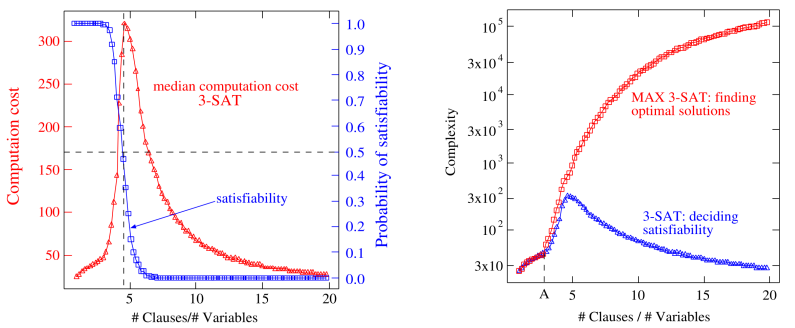
\includegraphics[scale=0.52]{images/max_sat_SAT.png}
    \caption{Plot delle fasi}
\end{figure}

Per $n\rightarrow\infty$ la transizione si concentra attorno $\alpha_c\approx 4.26$
\subsection{La transizione di fase per il VCP}
Il VCP esibisce una transizione di fase simile alla precedente quando $\frac{|x|}{|V|}$
incrementa.
\begin{itemize}
    \item Il tempo computazionale prima esplode, dopo cade.
    \item Per $n\rightarrow\infty$ la transizione si concentra attorno al valore critico.
\end{itemize}

\begin{figure}[H]
    \centering
    \includegraphics[scale=0.7]{images/phase_VCP.png}
    \caption{Fase del VCP}
\end{figure}

Quando $\frac{|x|}{|V|}$ è piccolo, alcuni vertici sono chiaramente necessari, problema risolto.
Quando $\frac{|x|}{|V|}$ è grande, molti vertici sono chiaramente necessari, problema risolto.

\subsection{Costo computazionale degli algoritmi euristici}
La complessità in tempo di un algoritmo euristico è solitamente:
\begin{itemize}
    \item \textbf{Strettamente polinomiale} (con esponenti bassi).
    \item \textbf{Abbastanza robusta} rispetto ai parametri secondari.
\end{itemize}
Perciò, la stima nel caso peggiore è buona nella media dei casi.
Le \textbf{metaeuristiche} utilizzano passi casuali o memoria:
\begin{itemize}
    \item La complessità è ben definita per componenti singoli dell'algoritmo.
    \item La complessità globale non è chiaramente definita, in teoria potrebbe
          essere estesa \textit{indefinitamente}, in pratica, è definita da una
          condizione imposta dall'utente.
\end{itemize}

\noindent\textit{Perché discutere ciò in un corso di algoritmi euristici ?}
\begin{itemize}
    \item Per guidare la ricerca dell'algoritmo corretto, un algoritmo corretto
          può essere efficiente in un caso specifico, ed inefficiente in un caso peggiore.
    \item Per mostrare che gli algoritmi euristici possono interagire proficuamente:
          poiché gli algoritmi euristici provvedono informazioni per migliorare gli algoritmi
          esatti (rendendoli più efficienti).
    \item Per mostrare che la kernelization migliora gli algoritmi euristici (diventano più efficienti
          ed efficaci).
    \item Per identificare \textit{a priori} le istanze più ardue, certamente non tutti
          gli algoritmi hanno le stesse istanze \textit{"complesse"}.
\end{itemize}

\section{Efficacia teorica}
\subsection{Efficacia di un algoritmo euristico}
Un algoritmo euristico è utile se è:
\begin{itemize}
    \item \textbf{Efficiente}, ovvero \textit{"costa"} molto meno di un algoritmo esatto.
    \item \textbf{Efficace}, ovvero restituisce \textit{"frequentemente"} una soluzione
          che è vicina a quella esatta.
\end{itemize}

Adesso vogliamo discute dell'efficacia degli algoritmi euristici, possiamo formalmente discutere
questo concetto introducendo il concetto di distanza di una soluzione rispetto ad una ottimale e la
frequenza (probabilistica) di ottenere una soluzione ottimale o quasi (rispetto ad una data distanza)
rispetto ad una soluzione ottima.
Queste caratteristiche possono essere combinate in una distribuzione a frequenza di soluzioni
più o meno vicine alla soluzione ottimale (andrà introdotto un concetto di distanza).

L'efficacia di un algoritmo euristico può essere investigata in due modi:
\begin{itemize}
    \item \textbf{Analisi teorica} (\textit{a priori}), provando che un algoritmo trova
          sempre o con una data frequenza soluzioni con una certa garanzia di qualità.
    \item \textbf{Analisi sperimentale} (\textit{a posteriori}), misurando le prestazioni dell'algoritmo
          su istanze di benchmark campionate per dimostrarne la presenza.
\end{itemize}

\subsection{Distanza tra le soluzioni}
Come detto precedentemente, dobbiamo dare un significato al concetto di distanza, e possiamo fornire
molteplici interpretazioni differenti.\\L'efficacia di un algoritmo di ottimizzazione euristico $A$
è misurata dalla \textbf{differenza} tra il valore $f_A(I)$ (la funzione obiettivo sull'istanza
$I$ calcolata da $A$) e il valore ottimale $f*(I)$ (la soluzione migliore per l'istanza $I$).

\subsubsection{Differenza assoluta}
Una possibile definizione iniziale tra due valori:
$$\widetilde{\delta}_A(I)=|f_A(I)-f^{*}(I)|$$
Seppure questa definizione è molto naturale ed ovvia, è raramente utilizzata in pratica poiché dipende
dall'unità di misura della funzione obiettivo: basa pensare di provare a minimizzare il tempo complessivo
nel caso del TSP e che lo si misuri in giorni. Si potrebbe provare ad utilizzare ore, minuti o secondi
anziché ed il valore di $\widetilde{\delta}_A(I)$ dipenderà fortemente da questa scelta. Questo sarà
valido quando la funzione obiettivo è un numero puro.

\subsubsection{Differenza relativa}
La seconda definizione è basata sull'idea che calcolare la differenza relativa rispetto alla soluzione
ottimale.
$$\delta_A(I)=\frac{|f_A(I)-f^*(I)|}{f^*(I)}$$
Questo è un approccio molto frequente nell'analisi sperimentale ed il suo vantaggio è che nel caso in
cui la funzione obiettivo abbia un unità di misura, allora il rapporto (\textit{rateo}) ottenuto sarà
un numero \textit{puro}.

\subsubsection{Rapporto di approssimazione}
Un terzo approccio, ampiamente utilizzato, è il rapporto di approssimazione:
$$\rho_A(I)=max\left[\frac{f_A(I)}{f^*(I)},\frac{f^*(I)}{f_A(I)}\right]\geq 1$$
Il quale include sia il problema di minimizzazione che di massimizzazione: nel caso in cui sia un
problema di minimizzazione, probabilmente $f*(I)<f_A(I)$ e viceversa per i problemi di massimizzazione.
Chiaramente è collegato alla differenza relazionale, in fatti nel caso dei problemi di minimizzazione:
$$\delta_A(I)=\rho_A(I)-1$$
La relazione esiste anche per i problemi di massimizzazione.

\subsection{Analisi teorica: garanzia di approssimazione}
Per garantire \textit{a priori} le prestazioni dell'algoritmo, l'idea è ancora una volta quella
di considerare il caso peggiore, proprio come per l'efficienza. In generale quando si applica
un algoritmo euristico il risultato $f_A(I)$ potrebbe essere un pessimo (distante) risultato
rispetto alla soluzione ottimale $f*(I)$, ma se l'algoritmo è buono la differenza non sarà
molto grande;

La differenza tra $f_A(I)$ e $f^*(I)$ è generalmente illimitata, ma per alcuni algoritmi è limitata:
\begin{itemize}
    \item \textbf{Approssimazione assoluta}: $$\exists\widetilde{\alpha}_A\in\mathbb{N}:\widetilde{\delta}_A(I)\leq\widetilde{\alpha}\text{ }\forall I\in\mathcal{I}$$
          Significa che la la distanza assoluta rispetto alla soluzione ottimale è limitata da
          un intero costante; un esempio è l'algoritmo di Vizing per la colorazione del grafo ($\widetilde{\alpha}=1$).

    \item \textbf{Approssimazione relativa}: $$\exists\alpha_A\in\mathbb{R}^+:\rho_A(I)\leq\alpha_A\text{ }\forall I\in\mathcal{I}$$
          Significa che il rapporto di approssimazione $\rho_A(I)$ ha un limite superiore delimitato da una costante reale $\alpha_A$.
          La cosa interessante è che la definizione può essere estesa a casi in cui una garanzia di approssimazione
          costante non può essere trovata considerando l'approssimazione come un valore ma come un'apposita funzione
          parametrizzata rispetto alla dimensione dell'istanza:
          $$\rho_A(I)\leq\alpha_A(n)\text{ }\forall I\in\mathcal{I}_n,n\in\mathbb{N}$$
\end{itemize}
In conclusione, è importante sottolineare che mentre l'efficienza e è necessariamente
dipendente dalla dimensione dell'istanza, l'efficacia \textit{potrebbe} non esserlo.

\subsubsection{Come ottenere una garanzia di approssimazione?}
Fornite le basi teoriche, ora possiamo descrivere in maniera generale un metodo per introdurre e
dimostrare un algoritmo con garanzia di approssimazione.\\ Per i problemi di minimizzazione,
si vuole dimostrare:
$$\exists\alpha_A\in\mathbb{R}:f_A(I)\leq\alpha_A f^*(I)\text{ }\forall I\in\mathcal{I}$$

Uno schema generalmente astratto è:
\begin{itemize}
    \item Trovare un modo per costruire una sottostima $LB(I)$ $$LB(I)\leq f^*(I)\text{,   }I\in\mathcal{I}$$
    \item Trovare un modo per costruire una sovrastima $UB(I)$ che sia in relazione con il coefficiente $\alpha_A$
          $$UB(I)=\alpha_A LB(I)\text{,   }I\in\mathcal{I}$$
    \item Trovare un algoritmo $A$ la cui soluzione non sia peggiore di $UB(I)$ $$f_A(I)\leq UB(I)\text{   }I\in\mathcal{I}$$
\end{itemize}

Se i tre passi sono stati completati e vengono trovati valori ed algoritmi adatti
$$f_A(I)\leq UB(I)=\alpha LB(I)\leq\alpha f^*(I)\text{   }\forall I\in\mathcal{I}\implies f_A(I)\leq\alpha_A f^*(I)\text{   }\forall I\in\mathcal{I}$$

La parte più complicata potrebbe essere il secondo passo, quindi affrontiamo mostrando un esempio.
\paragraph{Garanzia di approssimazione per il VCP: algoritmo 2-approssimato}: dato un grafo indiretto
$G=(V,E)$ trovare un sottoinsieme di vertici di cardinalità minima tale per cui ogni arco dell'arco
del grafo sia incidente.\\Definiamo:
\begin{itemize}
    \item Un insieme \textbf{"matching"}, tale per cui sia l'insieme degli archi non adiacenti.
    \item Un insieme \textbf{"maximal matching"}, è un insieme di tipo \textit{matching} tale che
          ogni altro arco del grafo è adiacente ad uno dei suoi archi.
\end{itemize}
Algoritmo di Matching:
\begin{enumerate}
    \item Costruire un \textit{maximal matching} $M\subseteq E$ scorrendo gli archi di $E$ e includendo in
          $M$ quelli che non sono adiacenti ad $M$ (ora ogni arco di $E\setminus M$ è adiacente ad un arco di $M$).
    \item L'insieme di vertici \textit{estremi} degli archi in \textit{matching} è la soluzione del VCP
          $$x_A := \bigcup_{(u,v)\in M}\{u,v\}$$ Può essere migliorata rimuovendo i vertici ridondanti.
\end{enumerate}

\begin{figure}[H]
    \centering
    \includegraphics[scale=0.5]{images/matching_0.png}
    \caption{Algoritmo di Matching - Passo 0 (stato iniziale del grafo)}
\end{figure}

\begin{figure}[H]
    \centering
    \includegraphics[scale=0.5]{images/matching_1.png}
    \caption{Algoritmo di Matching - Passo 1}
\end{figure}

\begin{figure}[H]
    \centering
    \includegraphics[scale=0.5]{images/matching_2.png}
    \caption{Algoritmo di Matching - Passo 2}
\end{figure}

\begin{figure}[H]
    \centering
    \includegraphics[scale=0.5]{images/matching_3.png}
    \caption{Algoritmo di Matching - Passo 3}
\end{figure}

Torniamo adesso alla garanzia di approssimazione. Un possibile limite inferiore è quello di includere nella soluzione
solamente uno dei vertici dell'arco nel \textit{maximal matching}: considero solo gli archi nel \textit{maximal
    matching} $M$.

È chiaro che il grafo consiste nei soli archi $e\in M$ ($G'=(V,M)$) solo \textit{metà} dei vertici inclusi nella
soluzione $x_A$ copre gli archi in $M$. In altre parole, la copertura ottimale dei vertici degli archi in $M$
è certamente più piccola della copertura ottimale di tutti gli archi in $E$.

Per fornire un esempio numerico, supponiamo che un certo grafo per il VCP abbia la soluzione ottimale $f^*=5$
(quindi $5$ vertici possono coprire tutti gli archi) e che l'algoritmo di matching trovi il matching massimale
con $3$ archi, quindi la soluzione dell'algoritmo sarà $f_A=2\cdot|M|=6$. Però coprire tutti gli archi in $M$
(considerare questo insieme come un grafo), basteranno $\frac{|M|}{2}=3$ vertici!

Il valore $\frac{|M|}{2}$ è un possibile limite inferiore (o \textit{lower bound}) per il nostro problema VCP:
$$LB(I)=\frac{|M|}{2}\leq f^*(I)$$
Ma c'è dell'altro: sappiamo che $x_A$ viene calcolato prima che sia una soluzione attualmente fattibile ed
è collegata a $LB(I)$:
$$f_A=2\cdot |M|=2\cdot LB(I)=UB(I)$$
Quindi abbiamo trovato sia il limite inferiore che quello superiore. Adesso forniamo una dimostrazione
formale che l'algoritmo di matching è \textbf{2-approssimato}:
\paragraph{Dimostrazione algoritmo di Matching 2-approssimato}, per prima cosa dimostriamo che la cardinalità
dell'insieme "matching" sia una sottostima $LB(I)$: la cardinalità di una copertura ottimale per un qualsiasi
sottoinsieme di archi $E'\subseteq E$ non supera quella di una copertura ottimale per $E$
$$|x^*_{E'}|\leq|x^*_E|$$
e la copertura ottimale di un qualsiasi insieme di matching $M$ ha cardinalità $\frac{|M|}{2}$, quindi
$$|M|\leq|E|\implies |x^*_M|\leq |x^*_E|\implies\frac{|M|}{2}\leq |x^*_E|\text{   }\forall M$$
$$LB(I)=\frac{|M|}{2}\leq |x^*_e|\text{ è un limite inferiore valido}$$
In parole, visto che l'insieme $M$ ha una cardinalità minore o uguale a quella di $E$, la soluzione ottimale
(la quale ha cardinalità esatta di $\frac{|M|}{2}$) ha una cardinalità minore o uguale a quella della
soluzione ottimale per l'insieme $E$, rendendola un valido limite inferiore.

Il fatto che $|M|$ stesso consiste in una sovrastima è provato dal fatto che la definizione dei vertici degli
archi in $M$ copre tutti gli archi in $E$, significa che l'insieme dei vertici $M$ consiste in una soluzione
fattibile (il che significa che è un limite superiore ed è un valore ottimale) e copre sia il "matching" che
gli archi adiacenti. Perciò $|M|=UB(I)=2\cdot LB(I)$ è una sovrastima.

La prova si conclude con il fatto che l'algoritmo restituisce soluzioni di valore $f_A(I)\leq UB(I)$, visto che
in $M$ potrebbero essere presenti dei vertici \textit{ridondanti} che possono essere rimossi. Questo
implica che $f_A(I)\leq 2\cdot f^*(I)\text{   }\forall I\in\mathcal{I}$, che è $\alpha_A=2$
\paragraph{Lo stretto legame tra stime inferiori e superiori}, \textit{sono presenti delle istanze $\overline{I}$ per
    il VCP tali che $f_A(\overline{I})=2\cdot f^{*}(\overline{I})$ utilizzando l'algoritmo di Matching?} Più
in generale, sono presenti delle istanze $\overline{I}$ tali che:
$$f_A(\overline{I})=\alpha_A f^*(\overline{I})$$
e se così, \textit{come sono le istanze $\overline{I}$?} In altre parole, dopo aver dimostrato che $f_A(I)$ è
in relazione con $f^*(I)$ attraverso $\alpha_A$, questo è \textbf{costante}, \textbf{preciso} e \textbf{importante}
o e \textit{"solo"} un limite superiore? Lo studio delle istanze $\overline{I}$ è utile per valutare se sono
rare o frequenti e per introdurre modifiche \textit{ad hoc} per migliorare l'algoritmo.
\paragraph{Garanzia di approssimazione per il TSP (disuguaglianza triangolare)}, consideriamo il TSP
con delle assunzione aggiuntive, ovvero che $G=(N,A)$ sia \textbf{completo} e che la funzione $c$ sia
simmetrica e soddisfi la \textbf{disuguaglianza triangolare}:
$$c_{ij}=c_{ij}\text{   }\forall i,j\in\mathbb{N}$$
e che
$$c_{ij}+c_{jk}\geq\text{   }\forall i,j,k\in\mathbb{N}$$
Il problema in generale, è fortemente NP-completo. Ma è anche fortemente NP-completo capire se le istanze
hanno una soluzione fattibile (non quale sia fattibile), ovvero se è presente un ciclo Hamiltoniano che visiti
tutti i nodi.

Sotto le precedenti assunzioni un algoritmo euristico può essere costruito con una garanzia di approssimazione
associata ad esso.
\paragraph{Algoritmo Double-tree}
\begin{enumerate}
    \item Considera il grafo completo e indiretto $G$
    \item Costruisci un minimo albero ricoprente $T^*=(N,X^*)$
    \item Fai una visita in pre-ordine di $T^*$ e costruisci due liste di archi:
          \begin{enumerate}
              \item $x$ sarà la lista degli archi utilizzata sia per la visita che per il backtracking:
                    questo è un ciclo che visita ogni nodo, possibilmente molteplici volte.
              \item $x'$ sarà la lista degli archi che connettono i nodi in pre-ordine con il primo nodo:
                    questo è un ciclo che visita ogni nodo esattamente una volta.
          \end{enumerate}
\end{enumerate}

\begin{figure}[H]
    \centering
    \includegraphics[scale=0.6]{images/TSP_double_tree_0.png}
    \caption{Double-tree per TSP - Passo 1 (grafo completo con archi omessi)}
\end{figure}

\begin{figure}[H]
    \centering
    \includegraphics[scale=0.6]{images/TSP_double_tree_1.png}
    \caption{Double-tree per TSP - Passo 2 (\textit{Minimo Albero Ricoprente} $T^*$)}
\end{figure}

\begin{figure}[H]
    \centering
    \includegraphics[scale=0.6]{images/TSP_double_tree_2.png}
    \caption{Double-tree per TSP - Passo 3.a (costruzione $x$)}
\end{figure}
$$x=\{
    A,C,F,H,\textcolor{blue}{F},I,\textcolor{blue}{F},\textcolor{blue}{C},
    D,G,L,\textcolor{blue}{G},E,\textcolor{blue}{G},
    \textcolor{blue}{D},B,\textcolor{blue}{D},\textcolor{blue}{C},A
    \}$$

\begin{figure}[H]
    \centering
    \includegraphics[scale=0.6]{images/TSP_double_tree_3.png}
    \caption{Double-tree per TSP - Passo 3.b (costruzione $x'$)}
\end{figure}

$$x'=\{A,C,F,H,U,D,G,L,E,B,A\}$$

La struttura è la stessa del VCP: una sottostima è trovata assieme al fattore di moltiplicazione
per costruire un limite superiore e quindi è provato che un algoritmo euristico può essere
dominato da questo limite superiore, il che significa che l'algoritmo euristico
è quasi sicuramente un fattore moltiplicato per la soluzione ottima. Andiamo a dimostrare
che l'algoritmo double-tree è 2-approssimato.
\paragraph{Dimostrazione algoritmo Double-tree 2-approssimato},
Rimuovendo un arco da un ciclo Hamiltoniano restituisce un percorso Hamiltoniano,
il quale è necessariamente più economico. Visto che un cammino Hamiltoniano ricopre tutti
i nodi, è effettivamente un albero ricoprente, e solitamente non di costo minimo. Quindi,
un attuale minimo albero ricoprente è sicuramente un limite inferiore sul costo di un
ciclo Hamiltoniano. La serie di nodi della visita DFS del MST (\textit{Minimum Spanning Tree})
assieme con i suoi archi di back tracking genera un ciclo Hamiltoniano nel grafo originale,
poiché è presente una coppia di archi diretti per ogni nodo (quindi ogni arco visitato nella
DFS esiste nel grafo originale).

Il costo di questo ciclo Hamiltoniano è necessariamente una sovrastima, visto che il
costo di tutti percorsi nel grafo rispetta la disuguaglianza triangolare; mentre la visita
restituisce, per esempio il percorso $A\rightarrow B\rightarrow C$, il grafo rispetta l'
uguaglianza triangolare scegliendo l'arco $A\rightarrow C$ la soluzione sarà di costo minimo.
Quindi, visto che $LB(I)$ è uguale al costo del MST ed il ciclo ha esattamente il doppio
degli archi del MST, abbiamo $UB(I)=2\cdot LB(I)$.

L'euristica è dominata da un limite superiore ed un qualsiasi circuito $x$ ha:
$$f_A(I)\leq UB(I)\leq 2\cdot LB(I)\leq 2\cdot f^*(I) \text{   }\forall I\in \mathcal{I}$$

\subsection{Inapprossimabilità}
Per un problema \textbf{inaprossimabile}, tutti gli algoritmi approssimati sono esatti, quindi
alcuni problemi non possono essere approssimati a meno che alcune proprietà della
complessità computazionale vengano verifica, cosa che è molto difficile che accada.

Per esempio, consideriamo la seguente famiglia di istanze del TSP che violano la
disuguaglianza triangolare nella seguente maniera:

\[c_{ij}=\begin{cases}
        0 & \forall (i,j)\in A_0\subset A   \\
        1 & \forall (i,j)\in A\setminus A_0
    \end{cases}
\]

ed il grafo è completo. Se una qualsiasi funzione di costo nullo ($f^*(I)=0$) viene trovata, significa che la
soluzione contiene solo archi in $A_0$ che compongono il ciclo Hamiltoniano. Quindi, in un senso, è presente
un grafo non-completo $G(N,A_0)$ che ha un ciclo Hamiltoniano come soluzione fattibile, tale che è lo stesso
per quello del grafo originale (questo significa che il grafo originale è il \textit{completamento} del nuovo
grafo).
Questo è bello finché una soluzione per il grafo completo viene trovata con costo nullo, allora potrai
veramente risolvere il problema del TSP nella forma decisionale anche sul grafo non completo, il quale
è un problema fortemente NP-completo. Quest non può essere fatto esattamente, a meno che $P=NP$, il
che è difficile. La funzione obiettivo di una qualsiasi istanza $\overline{I}$ è:
\[\begin{cases}
        f^*(\overline{I})=0     & \text{Se }A_0\text{ contiene un ciclo Hamiltoniano} \\
        f^*(\overline{I})\geq 1 & \text{Altrimenti}
    \end{cases}
\]

Non possiamo trovare una garanzia di approssimazione sul valore $\alpha$ per un algoritmo
polinomiale tale che:
$$f_A(I)\leq\alpha f^*(I)\text{  }\forall I\in\mathcal{I}$$
Poiché assumendo che sia possibile quello che accade è che se il grafo avesse un ciclo Hamiltoniano
di costo zero, allora necessariamente l'algoritmo di approssimazione restituirà un costo:
$$f^*(\overline{I})=0\Leftrightarrow f_A(\overline{I})=0$$
in parole povere, l'algoritmo di approssimazione risolve la versione decisionale del TSP nel
caso di un istanza con il grafo non-completo, questo è possibile risolvendo un problema
fortemente NP-completo in tempo polinomiale e dimostrando che $P=NP$. Visto che questo è molto
difficile che sia così, il problema il TSP è considerato un problema inaprossimabile.

\subsection{Schemi di approssimazione}
A volte è possibile trovare qualcosa meglio di una semplice approssimazione: per un qualsiasi
problema difficile è presente un algoritmo esaustivo che fornisce la migliore approssimazione
possibile garantendo $\alpha_A=1$ (in quanto esatto), ciò richiede tempo esponenziale $T_A$.

Gli algoritmi approssimati solitamente una garanzia di approssimazione peggiore ($\alpha_A >1$)
ma essi potrebbero richiedere tempo polinomiale $T_A$.

Ora nel mezzo di questi due casi si possono trovare molte cose, significa che al posto di un singolo algoritmo
polinomiale con tempo $T_A$ e garanzia $\alpha_A$ potrebbe essere presente una completa
famiglia di \textit{"differenti compromessi"} tra efficienza ed efficacia, che incrementano la
complessità computazionale e migliorano la garanzia di approssimazione.

\begin{itemize}
    \item Migliori e migliori garanzie di approssimazione: $\alpha_{A_1} > ... > \alpha_{A_r}$
    \item Peggiori e peggiori complessità computazionali: $T_{A_1}<...<T_{A_r}$
\end{itemize}

Tali famiglie di algoritmi sono chiamate \textbf{schemi di approssimazione}, i quali sono algoritmi
parametrici $A_\alpha$, che permettono di scegliere $\alpha$. Un esempio di questo è il problema KP.

\subsection{Oltre al caso peggiore}
Proprio come per l'efficienza, l'efficacia ha dei metodi di misurazione che sono approcci
differenti dal \textit{caso peggiore}. Potresti avere un brutto caso peggiore senza approssimazione
o un approssimazione $\alpha=1000000$ che restituisce una soluzione ottimale. Sono presenti differenti approcci.

\subsubsection{Parametrizzazione}
Anziché dividere le istanze per la dimensione, altri parametri $k_i$ possono essere identificati in maniera che
essi possano provvedere una garanzia di approssimazione che dipenda da $k_i$ e non sia costante.

\subsubsection{Caso medio}
Assume una probabilità di distribuzione sulle istanze e ne calcola il fattore di approssimazione desiderato (
l'algoritmo potrebbe avere delle brutte prestazioni solo su rare istanze).

\subsubsection{Randomizzazione}
Le operazioni dell'algoritmo dipendono non solo dall'istanza, ma anche dai numeri pseudocasuali, in maniera
che la soluzione diventa una variabile casuale la quale possa essere investigata (la complessità in tempo
potrebbe anch'essa essere casuale, ma solitamente non lo è).

Per un algoritmo casuale $A$, vengono considerate come variabili casuali $f_A(I)$ e $\rho_A(I)$. Un
\textbf{algoritmo di approssimazione casuale} ha un rapporto di approssimazione il cui valore desiderato
è limitato da una costante:
$$E[\rho_A(I)]\leq\alpha_A\text{  }\forall I\in\mathcal{I}$$

Considerando il problema Max-SAT: data una CNF, si vuole trovare l'assegnamento di verità per le variabili logiche
tale che soddisfi un sottoinsieme di peso massimo di formule.

Allora una algoritmo puramente casuale assegna ad ogni variabile $x_j(j=1,...,n)$:
\begin{itemize}
    \item Un valore $False$ con probabilità 0.5
    \item Un valore $True$ con probabilità 0.5
\end{itemize}

\paragraph{Approssimazione casuale per il Max-SAT} Sia $C_X\subseteq\{1,...,m\}$ il sottoinsieme
di formule soddisfatte dalla soluzione $x$. Il valore oggettivo $f(x)=f_A(I)$ è il peso totale
delle formule in $C_x$ ed il valore desiderato è:
$$E[f_A(I)]=E\left[\sum_{i\in \mathcal{C}_x}w_i\right] = \sum_{i\in \mathcal{C}}(w_i\cdot Pr[i\in \mathcal{C}_x])$$
Sia $k_i$ il numero di letterali della formula $i\in \mathcal{C}$ e $k_min = min\underset{i\in \mathcal{C}}{k_i}$

$$Pr[i\in \mathcal{C}_x]=1-\left(\frac{1}{2}\right)^{k_i}\geq 1-\left(\frac{1}{2}\right)^{k_{min}}\text{  }\forall i\in \mathcal{C}$$
$$\implies E[f_A(I)]\geq\sum_{i\in \mathcal{C}}w_i\cdot\left[1-\left(\frac{1}{2}\right)^{k_min}\right]=\left[1-\left(\frac{1}{2}\right)^{k_{min}}\right]\sum_{i\in \mathcal{C}}w_i$$
e visto che $E[\rho_A(I)]=f^*(I)/E[f_A(I)]$ e $f^*(I)\leq\sum_{i\in \mathcal{C}w_i}\text{  }\forall I\in\mathcal{I}$
uno ottiene:
$$E[\rho_A(I)]\leq 1/\left[1-\left(\frac{1}{2}\right)^{k_{min}}\right]\leq 2$$

\section{Valutazione empirica delle prestazioni}
Dopo la considerazione di un analisi algoritmica svolta \textit{a priori}, la quale consiste
nel dimostrare la presenza di alcune garanzie su alcuni aspetti dell'algoritmo che
sono stati studiati come il costo computazione della qualità delle soluzioni, ora
è possibile considerare l'analisi algoritmica \textit{a posteriori}.

Questo perché l'analisi a priori è complicata su diversi aspetti: nell'analisi dell'efficienza
il concetto è semplice mentre nell'analisi della qualità è molto più complicata,
poiché i "passi elementari" degli algoritmi non hanno una relazione diretta
con la qualità della soluzione. Inoltre, nel caso medio e della randomizzazione si richiede
un trattamento statistico.

L'analisi teorica può esser una pratica \textbf{insoddisfacente} quando le conclusioni sono basate
su \textbf{assunzioni non rappresentative}, come: un caso peggiore non frequente (molto difficile e
su istanze molto rare), oppure una distribuzione probabilistica delle istanze irrealistica.

\subsection{Analisi sperimentale}
Il metodo sperimentale è l'approccio tipico che viene utilizzato nella scienza con l'eccezione
della matematica, la quale è basata più su approcci formali, ma gli algoritmi sono l'eccezione
all'eccezione, visto che solo alcune proprietà legate alle prestazioni degli algoritmi possono
essere dimostrate e informazioni interessanti possono essere estrapolate dalle prestazioni pratiche.

Quindi abbiamo trovato un \textit{isola empirica} in un mare di formalismo.

L'approccio empirico consiste nell'osservare la realtà ed effettuare alcune assunzioni su come
la realtà "funzioni", questo formulando un \textbf{modello}. Dopo, una sequenza di passi
viene ripetuta fino ad ottenere un \textbf{modello soddisfacente}:

\begin{enumerate}
    \item Progettare esperimenti computazionali per validare il modello.
    \item Eseguire gli esperimenti e collezionare i risultati.
    \item Analizzare i risultati con metodi quantitativi.
    \item Revisionare il modello in base ai risultati ottenuti.
\end{enumerate}

\subsubsection{Modello}
\textit{Che cosa è un modello nel contesto dell'algoritmica?} In fisica un modello è una
legge che regola il comportamento di un fenomeno e, come analogia, nell'algoritmica
un modello è una legge che ipoteticamente regola il comportamento dell'algoritmo stesso.

Le leggi possono essere del tipo: assumere che la complessità computazionale
dell'algoritmo sia lineare, questo dipenderà da altri parametri come il massimo
grado divertici del grafo, ecc...

Questo è qualcosa che viene assunto basato sulla conoscenza dell'algoritmo ma anche su
un \textit{trend} esposto dall'approccio empirico.

L'analisi sperimentale degli algoritmi mira:
\begin{enumerate}
    \item Ottenere indici di efficienza ed efficacia compatti di un algoritmo.
    \item Paragonare gli indici di algoritmi differenti per ordinarli.
    \item Descrivere la relazione tra gli indici ed i valori parametrici delle istanze.
    \item Suggerire miglioramenti negli algoritmi.
\end{enumerate}

\subsubsection{Benchmark}
Visto che non tutte le istanze possono essere testate, viene definito un campione di
riferimento (\textbf{benchmark sample}): un campione significativo deve rappresentare differenti
\begin{itemize}
    \item Dimensioni, in particolare per l'analisi dei costi computazionali.
    \item Caratteristiche strutturale (\textit{densità, grado, diametro, ...}).
    \item Tipi
          \begin{itemize}
              \item di applicazione: logistici, telecomunicazioni, produzione, ...
              \item di generazione: realistici, artificiali, trasformazioni di altri problemi, ...
              \item di distribuzione probabilistica: uniforme, normale, esponenziale, ...
          \end{itemize}
\end{itemize}
Cercare un benchmark sample che sia "equiprobabile" non è significativo perché:
\begin{itemize}
    \item Le istanze di un insieme sono infinite.
    \item Gli insiemi infiniti non ammettono l'equiprobabilità (grande domanda della statistica).
\end{itemize}

Al contrario, noi possiamo:
\begin{itemize}
    \item Definire classi finite di istanze che sono:
          \begin{itemize}
              \item Sufficientemente difficile per essere istruttive.
              \item Sufficientemente frequenti in applicazione di interesse.
              \item Veloci abbastanza nella risoluzione, in modo da fornire dati sufficienti per le conclusioni.
          \end{itemize}
    \item Estrarre benchmark samples da queste classi.
\end{itemize}

\paragraph{Riproducibilità}\mbox{}\\
Il metodo scientifico richiede risultati riproducibili e controllabili. Quindi,
se vengono fatte delle indagini, è necessario assicurarsi che altre persone siano
in grado di replicare l'esperimento. Quindi, è necessario utilizzare \textbf{istanze
    pubblicamente disponibili} (o renderle pubblicamente disponibili), specificare i
dettagli di implementazione, il linguaggio di programmazione e il compilatore
dell'algoritmo implementato e i valori ambientali come la macchina utilizzata,
il sistema operativo e la memoria disponibile.

\subsection{Confronto di algoritmi euristici}
Un algoritmo euristico è migliore di un altro altro quando simultaneamente
\begin{itemize}
    \item Ottiene risultati migliori.
    \item Richiede meno tempo.
\end{itemize}
Algoritmi lenti con buoni risultati ed algoritmi veloci con brutti risultati
non possono essere paragonati in una maniera significativa. In alcune situazioni
specifiche il tempo computazionale può essere trascurato, precisamente quando
non si vuole fare alcun confronto ma si cerca di fare solo una stima e anche
quando si sa che i l tempo di calcolo è più o meno lo stesso (per conosciuti
motivi strutturali, ad es. due algoritmi uguali ma con qualche differenza nei
parametri).

\subsubsection{Descrivere le prestazioni di un algoritmo}
Per descrivere le prestazioni di un algoritmo un \textbf{metodo statistico} può essere
fornito. In particolare, l'idea è quella di modellare un algoritmo come se fosse un
esperimento casuale in cui i risultati dipendono dalla scelta di un oggetto
all'interno dello \textit{spazio di campionamento} (sample space), definito come
il campionamento delle istanze
$$\overline{\mathcal{I}}\subset \mathcal{I}$$
Il tempo computazionale $T_A(I)$ assieme alla differenza relativa $\delta_A(I)$
sono entrambe \textit{variabili casuali}.

Le proprietà statistiche delle variabili casuali $T_A(I)$ e $\delta_A(I)$ descrivono
le prestazioni dell'algoritmo $A$.

Quello che viene effettuato: anzichè considerare tutti i possibili valori del tempo
computazionale e tutti i possibili valori della differenza relativa, si descrivono
le variabili casuali con le loro proprietà statistiche, cosa che darà una descrizione
statistica delle prestazioni dell'algoritmo.

\subsection{Valutazione a posteriori dell'efficienza}
\subsubsection{Analisi del tempo computazionale (\textit{RTD diagram})}
Il diagramma \textit{"Run Time Distribution"} (RTD) è il grafico della funzione di
distribuzione $T_A(I)$ su $\overline{\mathcal{I}}$.
$$F_{T_A}(t)=Pr[T_A(I)\leq t]\text{  }\forall t\in\mathbb{R}$$
Visto che $T_A(I)$ dipende fortemente dalla dimensione di $n(I)$, significa che
diagrammi RTD significativi solitamente si riferiscono a benchmarks
$\overline{\mathcal{I}}_n$ con un $n$ fissato (e possibilmente fissati anche
altri parametri suggeriti dall'analisi del caso peggiore).
\begin{figure}[H]
    \centering
    \includegraphics[scale=0.35]{images/RTD_0.png}
    \caption{Diagramma \textit{Run Time Distribution}}
\end{figure}

Se tutti i parametri influenti vengono identificati e fissati, il diagramma RTD degenera
in una funzione a scala (ovvero, tutte le istanze richiedono lo stesso tempo).
\begin{figure}[H]
    \centering
    \includegraphics[scale=0.4]{images/RTD_stairs.png}
    \caption{RTD degenerato ina una \textit{step function}}
\end{figure}
Il diagramma RTD è:
\begin{itemize}
    \item \textbf{monotona non decrescente}, più istanze vengono risolte in più tempo.
    \item \textbf{graduale e continua verso destra}, il grafico aumento ad ogni $T(I)$.
    \item \textbf{uguale a $0$ per $t<0$}, nessuna istanza è risolta in tempo negativo.
    \item \textbf{uguale ad $1$ per $t\geq\underset{I\in\overline{\mathcal{I}}}{T(I)}$}, tutti vengono risolti con il tempo più grande.
\end{itemize}
Per benchmark sample, il disegno sembra continuo, ma non lo è.

Costruzione del RTD:
\begin{itemize}
    \item Eseguire l'algoritmo su ogni istanza $I\in\overline{\mathcal{I}}$
    \item Costruire l'insieme $T_A(\overline{\mathcal{I}})=\{T_A(I):I\in\overline{\mathcal{I}}\}$
    \item Ordinare $T_A(\overline{\mathcal{I}})$ non decrementando i valori $t_1 \leq ...\leq t_{|\overline{\mathcal{I}}|}$
    \item Disegnare i punti $\left(t_j,\frac{j}{|\overline{\mathcal{I}}|}\right)$ per $j=1,...,|\overline{\mathcal{I}}|$ ed
          i segmenti orizzontali (chiusi a sinistra, aperti a destra).
\end{itemize}

\subsubsection{Analisi del tempo computazionale (\textit{scaling diagram})}
Lo \textbf{scaling diagram} descrive la dipendenza di $T(I)$ sulla dimensione di $n(I)$
\begin{itemize}
    \item Genera una sequenza di valori di $n$ ed un campion $\overline{\mathcal{I}}_n$
          per ogni valore.
    \item Applica l'algoritmo ad ogni $I\in\overline{\mathcal{I}}_n\text{  }\forall n$
    \item Disegna tutti i punti $(n(I),T(I))$ o i punti medi $\left(n,\frac{\sum_{I\in\overline{\mathcal{I}}_n}T(I)}{|\overline{\mathcal{I}}_n|}\right)$
    \item Assumere una \textbf{funzione interpolante}.
    \item Stimare i parametri numerici della funzione interpolante.
\end{itemize}
\begin{figure}[H]
    \centering
    \includegraphics[scale=0.4]{images/interp_funct.png}
    \caption{Stima dei parametri rispetto alla funzione interpolante}
\end{figure}
L'analisi fornisce empiricamente un caso medio di complessità, con fattori di molteplicità
ben determinati (anziché $c_1$ e $c_2$), e non più grande del caso peggiore.

\subsubsection{Interpolazione dello \textit{scaling diagram}}
La famiglia corretta di funzioni interpolanti può essere suggerita, da:
\begin{itemize}
    \item Analisi teorica
    \item Manipolazione dei grafici
\end{itemize}
Solitamente l'\textbf{interpolazione lineare} è lo strumento corretto.
Il dragamma di scaling si trasofrma in una linea dritta quando
\begin{itemize}
    \item Un algoritmo esponenziale è rappresentato da una \textbf{scala semi logaritmica} (il logaritmo
          viene applicato solo sull'asse del tempo).
          $$\log_2 T(n)=\alpha n + \beta \Leftrightarrow T(n)=2^\beta(2^\alpha)^n$$

    \item Un algoritmo polinomiale è rappresentato da una scala logaritmica (il logaritmo viene
          applicato su entrambi gli assi).
          $$\log_2 T(n) = \alpha log_2 n + \beta \Leftrightarrow T(n) = 2^\beta n^\alpha$$
\end{itemize}

\subsection{Valutazione a posteriori dell'efficacia}
\subsubsection{Analisi della qualità della soluzione (\textit{SQD diagram})}
Il diagramma \textbf{Solution Quality Distribution} (SQD) è il grafico della funzione di distribuzione $\delta_A(I)$ su
$\overline{\mathcal{I}}$
$$F_{\delta_A}(\alpha) = Pr[\delta_A (I)\leq\alpha]\text{   }\forall\alpha\in\mathbb{R}$$
\begin{figure}[H]
    \centering
    \includegraphics[scale=0.4]{images/SQD_0.png}
    \caption{Diagramma \textit{Solution Quality Distribution}}
\end{figure}
Per un qualsiasi algoritmo, la funzione di distribuzione di $\delta_A(I)$
\begin{itemize}
    \item \textbf{Monotona non decrescente}: più casi vengono risolti con lacune peggiori.
    \item \textbf{graduale e continua a destra}: il grafo effettua un passo ad ogni $\delta(I)$
    \item \textbf{Uguale a $0$ per $\alpha <0$}: nessuna istanza viene risolta con lacune peggiori.
    \item \textbf{Uguale ad $1$ per} $\alpha\geq\underset{I\in\overline{\mathcal{I}}}{max}\delta_I$: tutte le istanze sono risolte all'interno della lacuna peggiore.
\end{itemize}

Se $A$ è un:
\begin{itemize}
    \item Algoritmo esatto, è una funzione a scala, uguale ad $1\text{   }\forall\alpha\geq0$
    \item Algoritmo $\overline{\alpha}$-approssimato, è una funzione uguale ad $1\text{   }\forall\alpha\geq\overline{\alpha}$
\end{itemize}
\paragraph{Costruzione del diagramma}
\begin{itemize}
    \item Eseguire l'algoritmo $\forall I\in\overline{\mathcal{I}}$
    \item Costruire l'insieme $\delta_A(\ovcal{I})=\{\delta_A(I):I\in\ovcal{I}\}$
    \item Ordinare $\delta_A(\ovcal{I})$ per valori non decrescenti : $\delta_1,...,\delta_{\ovcal{I}}$
    \item Disegnare i punti $\left(\delta_j,\frac{j}{|\ovcal{I}|}\right)$ per $j=1,...,|\ovcal{I}|$ ed
          i segmenti orizzontali (chiusi a sinistra, aperti a destra).
\end{itemize}

\begin{figure}[H]
    \centering
    \includegraphics[scale=0.45]{images/SQD_1.png}
\end{figure}

\subsubsection{Diagrammi SQD parametrici}
Dati i problemi teorici e pratici per costruire un campione significativo, il diagramma è parametrizzato
rispetto a:
\begin{itemize}
    \item Un parametro descrittivo delle istanze (dimensione, densità, ...)
    \item Un parametro di distribuzione probabilistica assunto per le istanze (varianza dei costi, ...)
\end{itemize}

\begin{figure}[H]
    \centering
    \includegraphics[scale=0.45]{images/SQD_2.png}
\end{figure}

Le conclusioni sono più limitate, ma il campione è più significativo, i \textbf{trend generali} possono
essere evidenziati.

\subsubsection{Confronto tra algoritmi utilizzando SQDs}
\textit{Come determinare quando un algoritmo è migliore di un altro?}
\begin{itemize}
    \item \textbf{Dominanza stretta}, ottiene migliori risultati su tutte le istanze.
          $$\delta_{A_2}(I)\leq\delta_{A_1}(I)\text{   }\forall I\in\mathcal{I}$$
    \item \textbf{Dominanza probabilistica}, la funzione di distribuzione ha valori più alti per
          tutti i valori di $\alpha$.
          $$F_{\delta_{A_2}}(\alpha)\geq F_{\delta_{A_1}}(\alpha)\text{   }\forall\alpha\in\mathbb{R}$$
\end{itemize}
Il seguente grafico non mostra alcuna dominanza, ma $A_1$ è meno \textit{"robusto"} di $A_2$, i
risultati di $A_1$ sono più spari di $A_2$.
\begin{figure}[H]
    \centering
    \includegraphics[scale=0.4]{images/SQD_3.png}
\end{figure}

\subsection{Descrizione statistica compatta}
Tutte le precedenti descrizioni prendono molto e sarebbe meglio avere dei numeri o una descrizione
compatta delle prestazioni di un algoritmo: come un indice statistico riguardante la differenza
relativa rispetto alla soluzione ottima. Questo coinvolge indici statistici classici di:
\begin{itemize}
    \item posizione, come il \textbf{sample mean} (\textit{mean} si riferisce alla media aritmetica di tutti
          i valori).
          $$\overline{\delta}_A = \frac{\sum_{I\in\ovcal{I}}\delta_A (I)}{|\ovcal{I}|}$$
    \item dispersione, come il \textbf{sample variance}.
          $$\overline{\sigma}^2_A = \frac{\sum_{I\in\ovcal{I}}(\delta_A(I)-\overline{\delta}_A)^2}{|\ovcal{I}|}$$

\end{itemize}
Questi indici tendono ad essere molto influenzati dai \textbf{valori anormali} (\textit{outliers}). Per
esempio, un algoritmo che $9/10$ fornisce la soluzione ottima ed $1/10$ fornisce dieci volte la
soluzione ottima, presenta chiaramente un valore anormale (questo non va bene). Utilizzando l'indice
"sample mean" avverrà la somma delle differenze $\frac{0+0+...+9}{10}=0.9$ restituendo un divario
medio del $90\%$, il quale non è una buona rappresentazione.

Altri indici statistici sono più \textit{"stabili"} e dettagliati:
\begin{itemize}
    \item \textbf{sample median}
    \item \textbf{sample quantiles}
\end{itemize}

\subsubsection{Boxplots}
Sia il sample median che il quantiles possono essere rappresentati utilizzando una rappresentazione
grafica chiamata \textbf{boxplot} (o diagramma a \textit{"scatola e baffi"} o \textit{"box and whiskers plot}).

\begin{figure}[H]
    \centering
    \includegraphics[scale=0.5]{images/boxplot.png}
    \caption{Esempio di boxplot}
\end{figure}
Supponiamo di avere 20 istanze nelle quali la relativa differenza spazia da $\approx4\%$ a $\approx11.5\%$,
rispettivamente nel caso migliore e nel caso peggiore.
All'interno del diagramma sono presenti cinque valori:
\begin{itemize}
    \item \textbf{sample median} (\textit{mediana}).
    \item \textbf{lower and upper sample quartiles} (\textit{quartile minore e superiore}, rispetto alla mediana).
    \item \textbf{extreme sample values}, (\textit{valori estremi}, escludendo gli \textit{outliers}).
\end{itemize}

La \textbf{mediana} è il valore che si trova oltre
metà delle istanze e sotto metà delle istanze: se il campione è costituito da un numero dispari di casi
la mediana è il valore dell'elemento nel "mezzo", nel nostro caso la mediana è qualcosa tra la decima
e l'undicesima istanza (un'altra opzione è quella di utilizzare proprio la decima istanza).

I quantili (considerando i \textit{quartili}) tipici utilizzati in un boxplot sono il
\textbf{primo ed il terzo}, cioè i valori che separano un quarto dell'osservazione dall'altra
di tre quarti; Per esempio su $20$ elementi il primo quartile corrisponde al quinto elemento
mentre il terzo al quindicesimo.

Una volta trovati i primi tre valori sono necessari altri due valori che sono i campioni estremi,
essi corrispondono al \textit{minimo ed al massimo}.

Questo è un diagramma interessante che fornisce sia la posizione che la dispersione del benchmark,
detto questo esattamente metà delle istanze cadrà nella "scatola" e le rimanenti tra la fine
della scatola ed i baffi. Questo diagramma è una descrizione semplificata del SQD e, visto che due
algoritmi possono essere paragonati utilizzando l'SQD, essi possono essere paragonati altrettanto
utilizzando i relativi boxplot.
\begin{figure}[H]
    \centering
    \includegraphics[scale=0.5]{images/boxplot_comparison.png}
    \caption{Confronto tra algoritmi attraverso i boxplot}
\end{figure}
Chiaramente, come mostrato in figure, il confronto è meno preciso di un diagramma SQD e meno
informazioni possono essere estratte, tuttavia delle interessanti conclusioni possono essere fatte.
In primis, prendendo sempre come esempio la figura sovrastante, gli $8$ boxplot rappresentano la
\textit{differenza relativa} su un campione fisso di un benchmark, dove i cerchi sono gli outliers.

Se paragoniamo $A_7$ e $A_8$, i due boxplot sono completamente separati, questo significa che tutte
le istanze dell'algoritmo $A_7$ hanno valori migliori, questa è la definizione di \textbf{dominanza stretta}.

Invece, si parla di \textbf{dominanza probabilistica} quando ognuno dei $4$ quartili di un boxplot
si trova sotto l'altro boxplot con cui ci si sta confrontando, come per esempio tra $A_2$ e $A_3$,
ma questa \textbf{non è una condizione sufficiente} (solo necessaria). Sempre considerando lo
stesso esempio potrebbe essere che un istanza parti dal baffo inferiore di $A_2$ e tutte le altre
si trovino esattamente nel primo quartile mentre accade l'opposto per $A_3$: in questo caso sicuramente
non può essere considerata la dominanza probabilistica.

\subsubsection{Relazione tra qualità e tempo computazioanle}
Un algoritmo euristico è migliore di un altro non quando restituisce risultati migliori ma quando
viene eseguito in un tempo minore. Se questo non accade, non si può dire che uno domini l'altro.

Tuttavia, sono presenti molto algoritmi che non trovano una singola soluzione come gli algoritmi
classici, ma quello che attuano è migliorare le soluzioni precedentemente trovate. Questo ne
consegue in terminazioni premature.

In particolare gli algoritmi con \textit{metaeuristiche} (passi casuali o meccanismi mnemonici)
hanno un tempo computazione $t$ fissato dall'utente e potenzialmente illimitato.
Sia $\delta_A(t,I)$:
\begin{itemize}
    \item La differenza relativa ottenuta da $A$ al tempo $t$ sull'istanza $I$.
    \item $+\infty$ se $A$ non ha ancora trovato una soluzione fattibile nel tempo $t$.
\end{itemize}
Come funzione del tempo di calcolo $t$, $\delta_A(t,I)$ è:
\begin{itemize}
    \item \textbf{monotona a scala non-crescente}.
    \item \textbf{costante dopo la terminazione regolare} $t\geq T(I)$ (se esiste).
\end{itemize}
\paragraph{Algoritmi randomizzati}\mbox{}\\
Se gli algoritmi metaeuristici hanno passi casuali, allora la differenza relativa è funzione del
seme casuale (\textit{random seed}) $\omega\in\Omega$ rendendo $\delta_A(t,I,\omega)$. Quando si effettua
il testing di un tale algoritmo, dovrebbe essere preso in considerazione che sono presenti due
elementi casuali: l'istanza $I$ estratta da $\ovcal{I}$ ed il random seed.

Durante il test questi parametri possono essere combinati o distinti, significa che in un esperimento
$I$ può essere fissato and un gruppo di semi $\overline{\Omega}$ viene testato, o al contrario, $\omega$
è fisso ed un campione di istanze $\ovcal{I}$ viene testato. I risultati su $\omega$ sono solitamente
riassunti fornendo entrambe la differenza minima $\delta_A^*(t,I)$ ed il tempo totale $|\overline{\Omega}|t$,
oppure la differenza media relativa $\overline{\delta}_A(t,I)$ ed il singolo tempo d'esecuzione $t$.

\subsubsection{Classificazione}
Ora abbiamo tutti gli elementi per fornire una \textbf{classificazione} abbastanza complicata per
algoritmi euristici, esatti ed approssimati. Questa vuole essere una classificazione di tutti
i tipi di algoritmi per problemi di ottimizzazione combinatoria

La relazione tra la qualità della soluzione e tempo computazionale permette di classificare gli
algoritmi in:
\begin{itemize}
    \item \textbf{completi}: per ogni istanza $I\in\mathcal{I}$, si trova l'ottimo in un tempo finito (un
          nome diverso per gli \textit{algoritmi esatti}).
          $$\exists\overline{t}_I\in\mathbb{R}^+ :\delta_A(I,t)=0 \text{  }\forall t\geq\overline{t}_I,I\in\mathcal{I}$$

    \item \textbf{probabilisticamente ed approssimativamente completi} (\textit{probabilistically approximately}):
          per ogni istanza $I\in\mathcal{I}$, si trova l'ottimo con una probabilità convergente ad $1$, rispetto
          ad una differenza relativa uguale a $0$, per $t\rightarrow\infty$
          (molti algoritmi metaeuristici randomizzati). Questi algoritmi non forniscono una soluzione ottima in un
          tempo finito, ma lo faranno se verrà fornito \textit{abbastanza tempo}.
          $$\lim_{t\rightarrow +\infty}Pr[\delta_A(I,t)=0]=1\text{  }\forall I\in\mathcal{I}$$

    \item \textbf{essenzialmente incompleti}: per alcune istanze di $I\in\mathcal{I}$, si trova
          la soluzione ottima con una probabilità strettamente $<1$ per $t\rightarrow +\infty$ (la maggior
          parte sono algoritmi greedy, algoritmi di ricerca locale, ...). Questi sono i "veri" algoritmi
          euristici.
          $$\exists I\in\mathcal{I}:\lim_{t\rightarrow +\infty}Pr[\delta_A(I,t)=0]<1$$
\end{itemize}

\paragraph{Classificazione generalizzata}\mbox{}\\
Un ovvia generalizzazione sostituisce la ricerca per l'ottimo con un dato livello di approssimazione:
$$\delta_A(I,t)=0\rightarrow\delta_A(I,t)\leq\alpha$$

\begin{itemize}
    \item \textbf{algoritmi $\alpha$-completi}: per ogni istanza $I\in\mathcal{I}$, trovano una soluzione $\alpha$-approssimata
          in un tempo finito (questi essenzialmente è una descrizione formale per gli algoritmi $\alpha$-approssimati).

    \item \textbf{algoritmi probabilisticamente ed approssimativamente $\alpha$-completi}: per ogni istanza $I\in\mathcal{I}$,
          trovare una soluzione $\alpha$-approssimata con una probabilità di convergenza ad $1$ per $t\rightarrow+\infty$.
    \item \textbf{algoritmi essenzialmente $\alpha$-completi}: per alcune istanze $I\in\mathcal{I}$ si trova
          una soluzione $\alpha$-approssimata con una probabilità strettamente $<1$ per $t\rightarrow +\infty$.
\end{itemize}
Concludendo, ogni algoritmo fornisce compromessi tra :
\begin{itemize}
    \item una misura della qualità, descritta dalla soglia $\alpha$.
    \item una misura del tempo, descritta dalla soglia $t$.
\end{itemize}

\subsection{Diagrammi complessi}
\subsubsection{La probabilità di successo}
Sia la \textbf{probabilità di successo} $\pi_{A,n}=Pr[\delta_A(I,t)\leq\alpha | I\in\mathcal{I}_{n,\omega}\in\Omega]$ essere
la probabilità che l'algoritmo $A$ trovi in un tempo $\leq t$ una soluzione con una divergenza $\leq\alpha$
di istanze con dimensione $n$.

I due importanti parametri li abbiamo già visti sono la soglia $t$ che è collegata
all'efficienza dell'algoritmo, e la soglia $\alpha$ legata all'efficacia dell'algoritmo.
\begin{figure}[H]
    \centering
    \includegraphics[scale=0.5]{images/prob_succ.png}
    \caption{Esempio di diagramma per la probabilità di successo}
\end{figure}
Come rappresentazione stiamo considerando il diagramma tri-dimensionale poiché
dipende da due variabili, la differenza relativa ed il tempo.

Da questo singolo diagramma è possibile estrarre altri tre classi di diagrammi "ausiliari",
questo tagliando lungo uno dei tre assi, quindi rispetto al tempo, qualità e probabilità.

\subsubsection{Qualified Run time Distribution diagram (QRTD)}
I diagrammi QRTD descrivono il profilo del tempo richiesto per raggiungere uno
specifico livello di qualità.
\begin{figure}[H]
    \centering
    \includegraphics[scale=0.55]{images/qrtd.png}
    \caption{Un esempio di diagramma QRTD}
\end{figure}
Se si sta cercando di raggiungere una certa qualità, allora il plot del diagramma
fornisce la probabilità di raggiungere tale qualità in un dato tempo. In
base alla tipologia di algoritmo l'ottimalità verrà raggiunta in dato tempo o
magari non raggiunta.
Il QRTD utile quando il tempo computazionale non è una risorsa scarsa.

Se l'algoritmo è:
\begin{itemize}
    \item completo, tutti i diagrammi raggiungono $1$ in un tempo finito (ottimalità sicuramente raggiunta).
    \item $\overline{\alpha}$-completo, tutti i diagrammi con $\alpha\geq\overline{\alpha}$
          raggiungono $1$ in tempo finito (l'ottimalità potrebbe essere raggiunta).
    \item $\overline{\alpha}$-incompleti, tutti i diagrammi con $\alpha\leq\overbrace{\alpha}$ non raggiungono $1$
          (l'ottimalità certamente non è raggiungibile).
\end{itemize}

\subsubsection{Timed Solution Quality Distribution diagram (TSQD)}
I diagrammi TSQD descrivono il profilo del livello di qualità
raggiunto in un dato tempo computazionale (qualità della soluzione relativa in un dato tempo).
\begin{figure}[H]
    \centering
    \includegraphics[scale=0.45]{images/tsqd.png}
    \caption{Un esempio di diagramma TSQD}
\end{figure}
Il TSQD utile quando il tempo computazionale non è una risorsa scarsa.

Se l'algoritmo è:
\begin{itemize}
    \item completo, tutti i diagrammi con un sufficiente $t$ sono funzioni a scala in $\alpha=0$.
    \item $\overline{\alpha}$-completo, tutti i diagrammi con un sufficiente $t$ raggiungono $1$ in $\alpha=\overline{\alpha}$.
    \item probabilisticamente approssimativamente $\overline{\alpha}$-completo, i diagrammi convergono ad $1$ per $\alpha=\overline{\alpha}$
    \item $\overline{\alpha}$-completo, tutti i diagrammi mantengono una probabilità $<1$ per $\alpha=\overline{\alpha}$
\end{itemize}

\subsubsection{Solution Quality Statistics over Time diagram (SQST)}
Finalmente possiamo disegnare le linee dei livelli associati con i differenti quantili, come
rappresentato nella sottostante figura.
\begin{figure}[H]
    \centering
    \includegraphics[scale=0.5]{images/sqst.png}
    \caption{Un esempio di diagramma SQST}
\end{figure}
Essi descrivono il compromesso tra qualità e tempo computazionale, nel caso di un algoritmo
\textit{robusto} le linee dei livelli sono molto vicine tra di loro. Questo è un diagramma
meno chiaro da leggere rispetto ad i precedenti. Supponiamo di essere interessati alla mediana
(linea puntinata), significa che vogliamo i risultati che impiegano almeno metà del tempo. Aspettando
$\approx20$ secondi una soluzione ottima potrà essere trovata (in metà del tempo rispetto ad un
quantile, tipo il terzo), invece
utilizzando un tempo minore una soluzione con qualità peggiore dovrà essere accettata.

\subsection{Wilcoxon's test}
I diagrammi ed i boxplot sono qualitativi, ma non sono veramente quantitativi. Per effettuare
una valutazione quantitativa della differenza empirica tra i due algoritmi può essere utilizzato
il \textbf{Wilcoxon's test} (il quale si concentra sull'efficacia seppur trascurando la robustezza).

\begin{enumerate}
    \item $f_{A_1}(I)-f_{A_2}(I)$ è uan variabile casuale definita su uno spazio delle istanze $\mathcal{I}$
    \item Formulare una \textbf{ipotesi nulla} (mancanza di relazione tra due fenomeni misurati) $H_0$
          secondo la quale la mediana teorica di $f_{A_1}(I).f_{A_2}(I)=0$
    \item Estrarre un campione di istanze $\ovcal{I}$ ed eseguire i due algoritmi su di esse, questo ci farà
          ottenere un campione di coppie di valori $(f_{A_1},f_{A_2})$.
    \item Calcolare la probabilità $p$ per ottenere i risultati osserva, o un risultato più "estremo",
          assumendo $H_0$ come vera.
    \item Impostare un livello significativo $\overline{p}$, il quale è la \textbf{probabilità massima accettabile}
          \begin{itemize}
              \item di rifiutare $H_0$ supponendo che sia vera.
              \item di considerare due mediane identiche come differenti.
              \item di considerare due algoritmi equivalenti come differentemente efficaci
                    (in riferimento alla mediana della divergenza).
          \end{itemize}
          e rifiutare $H_0$ quando $p<\overline{p}$
\end{enumerate}

I test statistici sono basati sulla formulazione di un ipotesi della \textbf{ipotesi nulla} $H_0$ in maniera
di comprendere la proprietà di osservare un certo comportamento empirico dato che tale ipotesi sia vera. In altre
parole, la nostra ipotesi nulla è che metà delle volte $f_{A_1}$ è meglio di $f_{A_2}$ e metà
delle volte è l'opposto. Questa è una buona  descrizione di due algoritmi equivalenti.

Valori tipici di $\overline{p}$ sono $5\%$ e $1\%$. Se la probabilità calcolata è più piccola,
allora $H_0$ è dimostrata falsa e rifiutata, e la mediana teorica tra gli algoritmi non sarà nulla.

\subsubsection{Ipotesi sul Wilcoxon's test}
Questo è un problema metodologico molto difficile. È un test \textbf{non parametrico}, il che
significa che non si sta ipotizzando su nulla a riguardo della distribuzione dei valori
testati. È utile valutare la prestazione degli algoritmi euristici, perché la distribuzione
dei risultati $f_A(I)$ è sconosciuta. È basato sulle seguenti ipotesi:
\begin{enumerate}
    \item Tutti i dati sono misurati su (almeno) una scala ordinata. Il valore specifico non
          è importante, solamente la dimensione relativa.

    \item I due data sets corrispondenti e derivano dalla stessa popolazione. Quindi applichiamo
          $A_1$ e $A_2$ alle stesse istanze estratte da $\mathcal{I}$.

    \item ogni coppia di valori è estratta indipendentemente da gli altri. Le istanze
          sono generate indipendentemente l'una dall'altra.
\end{enumerate}

La terza assunzione non è sempre verificata, quindi è necessario porre attenzione. Pensando
a qualche problema complicato come il Vehicle Routing problem. Generare differenti famiglie
di pesi sullo stesso grafo rende le istanza non proprio indipendenti l'una dall'altra.

Per eseguire il test devono essere seguiti i seguenti passi:
\begin{itemize}
    \item Calcolare la differenza assoluta $|f_{A_1}(I_i)-f_{A_2}(I_i)\text{   }\forall I_i\in\ovcal{I}$
    \item Ordinare quest'ultimi in ordine decrescente ed assegnare un \textbf{rango} (o \textit{rank})
          $R_i$ a ciascuno di essi.
    \item Sommare separatamente i ranghi delle coppie con una differenza positiva e quelli con
          una differenza negativa. Se l'ipotesi nulla $H_0$ risulta vera, allora le due somme dovrebbero
          essere uguali.
          \[
              \begin{cases}
                  W^+ =\sum_{i:f_{A_1}(I_i)>f_{A_2}(I_i)}R_i \\
                  W^- =\sum_{i:f_{A_1}(I_i)<f_{A_2}(I_i)}R_i
              \end{cases}
          \]
    \item La differenza tra $W^+-W^-$ permette di calcolare il valore di $p$: ognuna delle
          $|\ovcal{I}|$ differenze può essere positiva o negativa, sono quindi presenti $2^{|\ovcal{I}|}$
          possibilità. $p$ è la frazione con $|W^+-W^-|$ uguale o maggiore rispetto al valore osservato.
    \item Se $p<\overline{p}$, la differenze è significativa e:
          \begin{itemize}
              \item Se $W^<W^-$, l'algoritmo $A_1$ è migliore di $A_2$.
              \item Se $W^>W^-$, l'algoritmo $A_1$ è migliore di $A_2$.
          \end{itemize}
\end{itemize}

\subsubsection{Calcolo di $p$}
Il valore di $p$ è solitamente:
\begin{itemize}
    \item calcolato esplicitamente dall'enumerazione quando $|\ovcal{I}|<20$
    \item approssimato con una distribuzione normale quando $|\ovcal{I}|\geq 20$
\end{itemize}
\begin{figure}[H]
    \centering
    \includegraphics[scale=0.5]{images/p_val.png}
    \caption{Distribuzione del Wilcoxon's test per svariate dimensioni di campioni}
\end{figure}
Per esempio, supponiamo di avere tre istanze $I_1, I_2$ e $I_3$ le quali restituiscono
differenze con ranghi $1,2$ e $3$. La situazione più sbilanciata è quando $A_1$ o $A_2$
è sempre migliore dell'altro, quindi quando ci sono tre differenze positive o tre negative;
in altre parole potrebbe accadere che i ranghi $1,2$ e $3$ siano tutti ranghi di
differenze tutte positive o tutte negative.

Ogni valore quindi può essere "positivo" o "negativo" (nel senso che è un rango
di una differenza positiva o negativa), quindi sono presenti $2^3=8$ possibilità.

Ciascuna delle quali è generalmente equiprobabile, quindi gli $8$ casi possono essere
numerati, come nella figura in alto a sinistra. In un caso tutti sono positivi e restituisce
$W^+-W^-=(1+2+3)-0=6$; in un altro caso sono tutti negativi $W^+-W^-=0-(1+2+3)=-6$, e così via;
in due casi la differenza è $0$$W^+-W^-=(1+2)-3=3-(1+2)=0$.

    Ci si aspetta dall'ipotesi nulla di essere in uno dei due casi dove la differenza è uguale a $0$.
    Ma nel caso contrario, \textit{quale è la probabilità?} Assumendo che le due popolazioni
    siano le stesse così che la mediana sia su $0$, la probabilità di essere in una situazione
    di differenza \textbf{non equa o peggiore} corrisponde alla somma delle probabilità per
    ogni numerazione nel caso: per esempio, se la differenza restituita fosse $6$ la sua
    probabilità è $\frac{1}{8}$. Se la differenza ottenuta è $4$, la probabilità di ottenere
    ciò o peggio è $\frac{2}{8}$ e così via.

    Quindi può essere calcolata attraverso l'enumerazione, o se sono presenti molte istanze,
    la legge dei grandi numeri dice che va bene approssimare con una distribuzione normale.

    \paragraph{Possibili conclusioni}\mbox{}\\
    Il test di Wilcoxon può suggerire:
    \begin{itemize}
        \item che uno dei due algoritmi è significativamente migliroe dell'altro.
        \item che i due algoritmi sono statisticamente equivalenti.
    \end{itemize}
    In entrambi i casi è importante "tenere un occhio" su $p$, poiché è una risposta
    stocastica.

    Se il campione include istanze di tipi differenti, due algoritmi potrebbero essere
    complessivamente equivalenti, ma non equivalenti sulle singole istanze delle classi.
    Quindi se effettuo un test su $\delta_A(I)$ anziché $f_A(I)$? È una domanda aperta.
    I risultati possono essere differenti utilizzando $\delta_A(I)$ significa che dando
    un peso minore alle istanze che hanno una soluzione ottimale maggiore. Probabilmente,
    se il risultato del test è differente nei due casi, il testo è probabilmente non
    affidabile.

    \section{Euristiche costruttive}
    Adesso che abbiamo fornito un ampia panoramica dei problemi e dei metodi di valutazione
    degli algoritmi sia a priori che a posteriori, possiamo considerare la prima delle
    tre classi di euristiche, le \textbf{euristiche costruttive}.

    \subsection{Introduzione alle euristiche costruttive}
    Per comprendere questo tipo di euristica dobbiamo ricordarci che i problemi di ottimizzazione
    combinatoria ammettono delle soluzioni $x$ che sono sempre sottoinsiemi di
    un dato ground set $B$, il quale è un insieme finito.

    Il fatto che noi abbiamo sottoinsiemi suggerisce un possibile modo di costruire una soluzione,
    ed in particolare le euristiche costruttive consistono nell'iniziare da un insieme vuoto
    iniziale $\emptyset$ e man mano aggiungere un elemento alla volta finché non si \textit{intuisce}
    che non ha senso introdurre nuovi elementi, terminando così l'algoritmo.
    Analizziamo passo a passo questo processo, considerando il sottoinsieme $x^{(t)}$
    aggiornato da una euristica costruttiva:
    \begin{enumerate}
        \item Si inizia da un insieme vuoto: $x^{(0)}=\emptyset$ (il quale è ovviamente
              sottoinsieme di una qualsiasi soluzione ottima). Sappiamo già che attraverso la
              kernelization o utilizzando procedure di riduzione può essere dimostrato che
              alcuni elementi del ground set sono necessariamente inclusi in almeno una soluzione ottima.
              In tali casi, potrebbe essere una buona idea iniziare ad includere nel sottoinsieme originale
              questi elementi "forzati".

        \item Termina quando incontra una condizione di terminazione, il razionale di questa condizione
              consiste nel fatto che aggiungere un elemento nel sottoinsieme corrente non avrebbe alcun senso
              visto che non restituirebbe una soluzione ottima.

        \item Seleziona il \textit{"migliore"} elemento $i^{(t)}\in B$ tra quelli \textit{"accettabili"}
              allo step $t$.

        \item Aggiungi $i^{(t)}$ al sottoinsieme corrente $x^{(t)}:x^{(t+1)}:=x^{(t)}\cup\{ i^{(t)}\}$
        \item Tornare al passo $2$.
    \end{enumerate}

    \subsubsection{Il grafo di costruzione}
    Il grafo di costruzione (\textbf{construction graph}), è lo strumento di modellazione principale
    di questa costruttiva. Esso è un grafo diretto, costituito da nodi ed archi: i nodi di questo grafo
    costituiscono l'insieme $\mathcal{F}_A$ ($F$ sta per \textit{find}), il quale è anche conosciuto come
    \textbf{spazio di ricerca} (o \textit{search space}), il quale dipende dall'algoritmo $A$.

    In altre parole $\mathcal{F}_A$ dipende dal \textit{problema} che si vuole risolvere, ma per lo stesso
    problema possono esserci differenti spazi di ricerca corrispondenti a differenti
    algoritmi, quindi differenti euristiche costruttive.

    Lo spazio di ricerca è definito come la collezione di tutti i sottoinsiemi $x\subseteq B$ accettabili
    per l'algoritmo $A$.
$$\mathcal{F}_A\subseteq 2^B$$
Ogni \textit{nodo} è un sottoinsieme ed alcuni saranno le soluzioni mentre altri no. Siamo interessati nei
sottoinsiemi che sono accettabili ed utili. Gli \textit{archi} connettono coppie di nodi,
l'arco in se è la collezione di tutte le coppie $(x,x\cup\{i\})$ tali che
$x\in \mathcal{F}_A ,i\in B\setminus x$ e $x\cup\{i\}\in \mathcal{F}_A$. Quindi, gli archi connettono
un sottoinsieme della soluzione ad un sottoinsieme leggermente più grande che rappresenta l'estensione
di un sottoinsieme ancora accettabile che include un nuovo elemento.
\begin{figure}[H]
    \centering
    \includegraphics[scale=0.6]{images/cons_graph.png}
    \caption{Il grafo di costruzione visita una sequenza di sotto insiemi che porta alla soluzione ottima}
\end{figure}
Questo grafo è un \textbf{DAG} (\textit{Directed Acyclic Graph}). Ogni possibile esecuzione di
$A$ è un \textbf{percorso massimo} del grafo di costruzione (contando sia il sottoinsieme
vuoto che un sottoinsieme la cui estensione non può essere accettata).

Il rettangolo del grafo di costruzione rappresenta le $2^B$, ovvero tutti i possibili
sottoinsiemi del ground set $B$. Questa collezione di sottoinsiemi
è partizione in classi che dipendono dalla loro cardinalità, quindi la prima classe (quella
più a sinistra) contiene solamente un possibile sottoinsieme, ovvero quello contenente l'insieme
vuoto $\emptyset$ (contenente tutti i sottoinsiemi di $0$ elementi). Nella seconda classe
dei sottoinsiemi possibili si trovano gli elementi singoli, poi le coppie, ecc. Sono
presenti $n+1$ classi che vanno da cardinalità $0$ fino a $n$. All'interno dell'insieme
potenza (o dei sottoinsiemi possibili), è presente lo spazio di ricerca degli algoritmi $\mathcal{F}_A$,
il quale contiene alcuni sottoinsiemi che sono considerati \textit{"utili"} per l'algoritmo: in
particolare contiene l'insieme vuoto (l'algoritmo parte da quello), e altri insiemi che ha senso
tenere conto.

Solitamente sottoinsiemi che sono al di fuori dello spazio di ricerca sono quelli che non hanno senso di
essere fissati, visto che non sono fattibili o perché non sono particolarmente "interessanti" ed
ogni altro sottoinsieme che non può essere raggiunto da $\mathcal{F}_A$ non è rilevante. Come prima
l'insieme delle soluzioni fattibili viene denotato con $X$, e l'insieme delle soluzioni ottime $X^*$.

Nell spazio di ricerca è presente un insieme di archi che connettono coppie di nodi, il secondo nodo
della coppia corrisponde al primo sottoinsieme della coppia più un certo elemento.

Come è possibile vedere dalle figure partire dal sottoinsieme vuoto è una soluzione accettabile,
le soluzioni non \textit{accettabili} si trovano al di fuori dello spazio di ricerca, e di fatti
non sono presenti archi che vanno al di fuori di questo. Quindi, ogni esecuzione di un algoritmo è un
percorso massimo all'interno del grafo di costruzione, che parte dal sottoinsieme vuoto e raggiunge
una soluzione, la quale idealmente dovrebbe essere ottimale o almeno fattibile. Nel caso ottimale,
il percorso termina quando incontra una soluzione ottima, questo è il caso degli
algoritmi di Dijkstra, Prim, Kruskal.
\begin{figure}[H]
    \centering
    \includegraphics[scale=0.8]{images/cons_graph_1.png}
    \caption{Il grafo di costruzione visita una sequenza di sotto insiemi che porta ad una soluzione
        fattibile ma non ottimale}
\end{figure}

Negli altri casi, come nella figura sovrastante, il percorso potrebbe non terminare in una soluzione
ottima ma fattibile $x\in X$, questo è il caso degli algoritmi euristici come quelli usati per
KP e MDP.
\begin{figure}[H]
    \centering
    \includegraphics[scale=0.8]{images/cons_graph_2.png}
    \caption{Il grafo di costruzione visita una sequenza di sotto insiemi che porta ad una soluzione non fattibile}
\end{figure}
Il percorso potrebbe terminare in una soluzione non fattibile $x\notin X$ (ma accettabile poiché presente
nello spazio di ricerca), come per esempio il TSP su un grafo non completo.

\paragraph{Esempio di costruzione di grafi}\mbox{}\\
Un esempio di grafo di costruzione è quello per il TSP per trovare il Nearest-Neighbour in
un grafo completo. L'idea è quella di iniziare con un insieme di archi vuoto, quindi $x^{(0)}=\emptyset$,
e sono presenti $n-1$ archi uscenti.

La costruzione del grafo sarà un albero con $n-1$ archi e $n$ nodi; il numero di percorsi dall'insieme
vuoto alle foglie sarà esattamente $(n-1)!$, questo è il numero delle possibili esecuzioni
dell'algoritmo.

\paragraph{Proprietà dello spazio di ricerca}\mbox{}\\
\begin{itemize}
    \item Include l'insieme vuoto $\emptyset\in\mathcal{F}_A$, visto che ogni algoritmo generalmente
          inizia da quello.

    \item In generale include l'insieme delle soluzioni fattibili $X\subseteq\mathcal{F}_A$, a volte
          alcune soluzioni possono essere rimosse da esso nel caso in cui risultino ovviamente non ottimali:
          per esempio l'SCP dove inizia con un insieme vuoto di colonne ogni colonna è a aggiunta, in un
          dato punto la soluzione fattibile viene raggiunta ma non ha senso aggiungere
          altre colonne perché i nuovi sottoinsiemi saranno fattibili ma anche più costosi.

    \item I sottoinsiemi di $\mathcal{F}_A$ devono essere raggiungibili dal punto di partenza,
          altrimenti non avrebbe senso aggiungere una soluzione che non è raggiungibile dall'inizio. Un
          insieme candidato è la collezione delle \textbf{soluzioni parziali}, che sono le soluzioni
          generalmente non fattibili ma sono sottoinsiemi di soluzioni fattibili. Seguire una soluzione
          parziale fornisce almeno un percorso per una soluzione fattibile $\in X$.

\end{itemize}
\paragraph{Esempi di spazi di ricerca}\mbox{}\\
Lo spazio di ricerca potrebbe include tutte le soluzioni fattibili tali che:
$$\mathcal{F}_A\equiv X$$
come nel KP; potrebbe includere tutte le soluzioni parziali e tutte le soluzioni fattibili, tale che:
$$\mathcal{F}_A\equiv \bigcup_{x\in X} 2^x$$
per esempio nel MDP, nel quale non solo i sottoinsiemi dei $k$ punti sono considerati ma anche
quelli più piccoli o nell'algoritmo di Kruskal; lo spazio di ricerca potrebbe includere solo
alcune soluzioni parziali:
$$\mathcal{F}_A\subset \bigcup_{x\in X} 2^x$$
un esempio di questo è l'algoritmo di PRim per MSP, il quale non consider tutte le soluzioni
parziali ma considera un albero che è in aumento rimanendo connesso finché non diventa ricoprente.
Le soluzioni possono essere definite come uno speciale sottoinsieme non sufficiente per garantire
la fattibilità:
$$ U_{x\in X}2^x \mathcal{F}_A$$
un esempio di questo è il TSP, dove $\mathcal{F}_a$ può essere definito su tutti i
sottoinsiemi di archi che non includono diramazioni o sotto percorsi, non può
essere definito come "tutti i sottoinsiemi che fanno parte delle soluzioni fattibili"
visto che è un problema di decisione NP-completo.

\subsection{Condizione di terminazione}
Un euristica costruttiva $A$ termina in due casi. Quando il sottoinsieme corrente $x^{t}$
non può essere esteso senza che lasci lo spazio di ricerca $\mathcal{F}_A$ :
$$x^{(t)}\cup\{i\}\notin\mathcal{F}_A\text{   }\forall i\in B\setminus x^{(t)}$$
o in maniera pressoché equivalente, non ha un arco uscente:
$$\Delta_A^+(x^{(t)})=\{i\in B\setminus x^{(t)}:x^{(t)}\cup\{i\}\in\mathcal{F}_A\}$$

Sono possibili differenti comportamenti:
\begin{itemize}
    \item Talvolta tutti i sottoinsiemi visitati sono fattibili (es. KP).
    \item Di solito l'ultimo sottoinsieme è l'unica soluzione fattibile.
    \item $x^{(t)}$ potrebbe muoversi dentro e fuori $X$ (o $X^*$), seppur improbabile.
\end{itemize}

\subsection{Struttura di algoritmi euristici costruttivi}
\begin{algorithm}[H]
    \caption{Pseudo codice - Euristica Costruttiva}
    \label{alg:cons_heu}
    \begin{algorithmic}
        \State $x:=\emptyset$
        \State $x^*:=\emptyset$

        \If{$x\in X$}
        \State $f^*:=f(x);$
        \Else
        \State{$f^*:=+\infty;$}
        \EndIf

        \While{$\Delta_A^+(x)\neq\emptyset$}
        \State $i:=arg\underset{i\in\Delta_A^+(x)}{min}\varphi(i,x);$
        \State $x:x\cup\{i\};$
        \If{$x\in X$ and $f(x)<f^*$}
        \State $x^* := x;$
        \State $f^* := f(x);$
        \EndIf
        \EndWhile
        \State $Return(x^*.f^*);$
    \end{algorithmic}
\end{algorithm}

Il percorso (la sequenza di sottoinsiemi) visitato dall'algoritmo è determinato
da:
\begin{itemize}
    \item l'insieme $\Delta_A^+(x)\subseteq B\setminus x$, il quale è derivato
          dal grafo di costruzione.
    \item il criterio di selezione $\varPhi_A:B\times \mathcal{F}_A\implies\mathbb{R}$ utilizzato
          per selezionare l'elemento $i$ da aggiungere al sottoinsieme corrente $x^{(t)}$ per generare
          $x^{(t+1)}$, che può essere visto come una funzione peso su gli archi $(x,x\cup {i})$.
\end{itemize}
La soluzione restituita è quella migliore visitata durante l'esecuzione (solitamente è l'ultima).

\subsection{Definizione del grafo di costruzione}
Idealmente, lo spazio di ricerca $\mathcal{F}_A$ dovrebbe includere:
\begin{itemize}
    \item Il sotto insieme vuoto $\empty \in \mathcal{F}_A$
    \item Tutte le soluzioni possibili $X\subseteq\mathcal{F}_A$ (questo escludendo
          le soluzioni non ottime).
    \item solo sottoinsiemi raggiungibili da $\emptyset$ (i sottoinsiemi non raggiungibili sono inutili).
\end{itemize}
I candidati naturali sono le soluzioni parziali (sottoinsiemi delle soluzioni fattibili), ma questi
richiedono un test di inclusione veloce per rispondere alla domanda:
\textit{il sottoinsieme $x^{(t)}$ è una soluzione parziale?} o meglio $\exists x \in X : x^{(t)}\subseteq x?$
o almeno dare un fast update test: sia $x^{(t)}$, allora $x^{(t)} \cup \{i\}\in\mathcal{F}_A?$
Sfortunatamente, questo problema generalizza la fattibilità del problema: \textit{è qui presente qualsiasi soluzione fattibile?}.
Questo potrebbe essere un problema NP-completo, in questo caso si ha necessità di rilassare lo spazio di ricerca.

Se la funzione obiettivo potesse essere estesa da $X$ a $\mathcal{F}_A$, allora sembrerebbe naturale
utilizzare la funzione obiettivo come \textbf{criterio di selezione}.
$$\varphi(i,x)=f(x\cup\{i\})$$
\begin{algorithm}[H]
    \caption{Pseudo codice - Euristica Costruttiva (funzione obiettivo)}
    \label{alg:cons_heu_fx}
    \begin{algorithmic}
        \State $x:=\emptyset$
        \State $x^*:=\emptyset$

        \If{$x\in X$}
        \State $f^*:=f(x);$
        \Else
        \State{$f^*:=+\infty;$}
        \EndIf

        \While{$\Delta_A^+(x)\neq\emptyset$}
        \State $i:=arg\underset{i\in\Delta_A^+(x)}{min}f(x\cup\{i\});$
        \State $x:x\cup\{i\};$
        \If{$x\in X$ and $f(x)<f^*$}
        \State $x^* := x;$
        \State $f^* := f(x);$
        \EndIf
        \EndWhile
        \State $Return(x^*.f^*);$
    \end{algorithmic}
\end{algorithm}

\subsection{Il problema dello zaino frazionario (FKP)}
Selezionando da un insieme di oggetti di volume identico un sottoinsieme di
valore massimo tale che possa essere contenuto all'interno dello zaino, il quale dispone di una
capacità massima limitata.

In questo problema la capacità impone un vincolo sulla cardinalità delle possibili soluzioni,
esse sono $|x|\leq\lfloor \frac{V}{v}\rfloor$.
$$\varphi(i,x)=f(x\cup\{i\})$$
\begin{algorithm}[H]
    \caption{Pseudo codice - GreedyFKP}
    \begin{algorithmic}
        \State $x:=\emptyset$
        \State $x^*:=\emptyset$

        \If{$x\in X$}
        \State $f^*:=f(x);$
        \Else
        \State{$f^*:=+\infty;$}
        \EndIf

        \While{$|x|<\lfloor\frac{V}{v}\rfloor$}
        \State $i:=arg\underset{i\in B\setminus x}{max}\phi_i;$
        \State $x:x\cup\{i\};$
        \If{$x\in X$ and $f(x)<f^*$}
        \State $x^* := x;$
        \State $f^* := f(x);$
        \EndIf
        \EndWhile
        \State $Return(x^*.f^*);$
    \end{algorithmic}
\end{algorithm}
Definiamo $\mathcal{F}_A = X$, dove il sottoinsieme $x$ può essere esteso finché $|x|<\lfloor\frac{V}{v}\rfloor$.
Un qualsiasi elemento di $B\setminus x$ estende $x$. La funzione obiettivo è additiva, e quindi:
$$f(x\cup\{i\})=f(x)+\phi_i\implies arg\underset{i\in B\setminus x }{max} f(x\cup\{i\}) = arg\underset{i\in B\setminus x }{max}\phi_i$$
L'ultimo sottoinsieme visitato è la migliore soluzione trovata.
Consideriamo il seguente esempio:
\[
    \begin{tabular}{c | c c c c c c c}
        B      & a & b & c & d & e & f \\
        \midrule
        $\phi$ & 7 & 2 & 4 & 5 & 4 & 1 \\
    \end{tabular}
\]
$$v_i=1\text{ }\forall i\in B$$
$$V=4$$
L'algoritmo eseguirà i seguenti step:
\begin{itemize}
    \item $x:=\emptyset;$
    \item Dato che $|x|=0<4$ allora calcola $i:=a$ ed aggiorna $x:=\{a\};$
    \item Dato che $|x|=1<4$ allora calcola $i:=d$ ed aggiorna $x:=\{a,d\};$
    \item Dato che $|x|=2<4$ allora calcola $i:=c$ ed aggiorna $x:=\{a,c,d\};$
    \item Dato che $|x|=3<4$ allora calcola $i:=e$ ed aggiorna $x:=\{a,c,d,e\};$
    \item Dato che $|x|\nless 4$, allora termina.
\end{itemize}
Questo algoritmo trova sempre la soluzione ottima.
\subsection{Il problema dello zaino (KP)}
Select from a set of object od different volume a maximum value subset which could be contained
on knapsack of limited capacity.
\begin{algorithm}[H]
    \caption{Pseudo codice - Greedy KP}
    \begin{algorithmic}
        \State $x:=\emptyset$
        \State $x^*:=\emptyset$
        \State $f*=0$

        \While{$\exists i \in B\setminus x :v_i\leq V-\sum_{j\in x}v_j$}
        \State $i:=arg\underset{\exists i \in B\setminus x :v_i\leq V-\sum_{j\in x}v_j}{max}\phi_i;$
        \State $x:x\cup\{i\};$
        \EndWhile
        \State $Return(x,f(x));$
    \end{algorithmic}
\end{algorithm}
Definire $\mathcal{F}_A = X$, solo alcuni elementi di $B\setminus x$ estendono la fattibilità di $c$
$$\Delta_A^+(x)=\{i\in B\setminus x:\sum_{j\in x}v_j+v : i \leq V\}$$

La funzione obiettivo è additiva e quindi
$$f(x\cup{i})=f(x)+\phi_i\implies arg\underset{i\in\Delta_A^+(x)}{max}f(x\cup\{i\})=arg\underset{i\in\Delta_A^+(x)}{\phi_i}$$
L'ultimo sottoinsieme visitato è la migliore soluzione trovata.
\[
    \begin{tabular}{c | c c c c c c c}
        B      & a & b & c & d & e & f \\
        \midrule
        $\phi$ & 7 & 2 & 4 & 5 & 4 & 1 \\
        v      & 5 & 3 & 2 & 3 & 1 & 1 \\
    \end{tabular}
\]
L'algoritmo esegue i seguenti step:
\begin{itemize}
    \item $x:=\emptyset;$
    \item Dato che $\Delta_A^+\neq\emptyset$ selezionare $i:=\{a\};$ ed aggiornare $x:=\{a\};$
    \item Dato che $\Delta_A^+\neq\emptyset$ selezionare $i:=\{d\};$ ed aggiornare $x:=\{a,d\};$
    \item Dato che $\Delta_A^+ = \emptyset$, terminare.
\end{itemize}
Questo algoritmo non trova una soluzione ottima
\subsection{Maximum Diversity Problem}
Selezionare da un insieme di punti un sottoinsieme di $k$ tale che la somma delle distanza
fra le coppie di questo insieme sia massima.
\begin{algorithm}[H]
    \caption{Pseudo Codice - GreedyMDP}
    \begin{algorithmic}
        \State $x:=\emptyset$
        \While{$|x|<k$}
        \State $i:=arg\underset{i \in B\setminus x}{max}\sum_{j\in x}d_{ij};$
        \State $x:x\cup\{i\};$
        \EndWhile
        \State $Return(x,f(x));$
    \end{algorithmic}
\end{algorithm}

Definire lo spazio di ricerca $\mathcal{F}_A$ come l'insieme di tutte le soluzioni parziali. Il
sottoinsieme $x$ può essere esteso finché viene soddisfatta la condizione del problema $|x|<k$.
Un qualsiasi elemento di $B$ estende $x$ in una maniera fattibile. La funzione obiettivo è quadratica:
$$f(x\cup\{i\})=f(x)+2\sum_{j\in x}d_{ij}+d_{ii}\implies arg\underset{i\in B\setminus x}{max}f(x\cup \{i\})=arg\underset{i\in B\setminus x}{max}\sum_{j\in x} d_{ij}$$
L'ultimo sotto insieme visitato è la soluzione migliore (è l'unica fattibile) trovata.

\begin{figure}[H]
    \centering
    \includegraphics[scale=0.5]{images/MDP_construct.png}
    \caption{Maximum Diversity Problem}
\end{figure}

L'algoritmo ha due grossi svantaggi:
\begin{itemize}
    \item Al primo passo, tutti i punti sono equivalenti.
    \item Il risultato finale non è ottimale anche se: il primo passo seleziona la coppia di
          punti più distanti o l'algoritmo viene ripetuto selezionando ogni punto come il primo.
\end{itemize}

\subsubsection{Travelling Salesman Problem}
Dato un grafo diretto ed una funzione di costo definita su gli archi, trovare il ciclo di costo
minimo che sia in grado di visitare tutti i nodi del grafo.

Lo spazio di ricerca $\mathcal{F}_A$ è definito come la collezione di tutti i sottoinsiemi di archi che
formano un particolare sotto percorso e mantengono il grado dei nodi $\leq 1$, per tutti i nodi (è
un sovra insieme di tutte le soluzioni parziali).
Il criterio di selezione è la funzione obiettivo, essendo additiva.

\begin{algorithm}[H]
    \caption{Pseudo Codice - GreedyTSP}
    \begin{algorithmic}
        \State $x:=\emptyset$
        \State $x*:=\emptyset$
        \State $f*:=\infty$
        \While{$\Delta_A^+(x)\neq \emptyset$}
        \State $i:=arg\underset{i \in \Delta_A^+(x)}{min}\;$
        \State $x:x\cup\{i\};$
        \EndWhile
        \If {$x\in X$}
        \State $x^*:=x;$
        \State $f^*:=f(x);$
        \EndIf
        \State $Return(x*,f^*);$
    \end{algorithmic}
\end{algorithm}
Solo l'ultimo insieme visitato può essere fattibile (se trovato!).
Per semplicità consideriamo un grafo simmetrico.
\begin{figure}[H]
    \centering
    \includegraphics[scale=0.5]{images/TSP_simm.png}
    \caption{TSP grafo simmetrico}
\end{figure}
L'algoritmo eseguirà i seguenti passi:
\begin{itemize}
    \item $x:=\emptyset;$
    \item Visto che $\Delta_A^+(x)\neq\emptyset$ selezioniamo $i:=(3,5)$ ed aggiorniamo $x;$
    \item Visto che $\Delta_A^+(x)\neq\emptyset$ selezioniamo $i:=(2,4)$ ed aggiorniamo $x((5,3)\notin\Delta_A^+(x));$
    \item Visto che $\Delta_A^+(x)\neq\emptyset$ selezioniamo $i:=(5,2)$ ed aggiorniamo $x((4,2)\notin\Delta_A^+(x));$
    \item Visto che $\Delta_A^+(x)\neq\emptyset$ selezioniamo $i:=(4,1)$ ed aggiorniamo $x:$
          notare che $(2,5),(4,5),(5,4),(3,4)$ e $(4,3)\notin \Delta_A^+(x)$
    \item Visto che $\Delta_A^+(x)=\emptyset$, terminiamo.
\end{itemize}
L'algoritmo non trova una soluzione fattibile, ma una soluzione fattibile esiste: aggiungendo
l'arco $(1,3)$ (quello tratteggiato in figura) permette di trovare una soluzione fattibile anche
nel caso in cui costi $100$ (seppur non ottima).
\subsection{Riassumendo}
Un'euristica costruttiva $A$ trova:
\begin{itemize}
    \item Una soluzione ottimale quando $\Delta_A^+(x^{(t)})$ e $\varphi_A(i,x)$ garantiscono
          che il sotto insieme corrente $x^{(t)}$ sia sempre incluso almeno in una soluzione ottima.
    \item Una soluzione fattibile quando $\Delta_A^+(x^{(t)})$ garantisce che il sottoinsieme
          corrente $x^{(t)}$ sia sempre incluso in almeno una soluzione fattibile.
    \item Un soto insieme generale quando queste proprietà sono perse ad un passo $t$.
\end{itemize}
Un algoritmo costruttivo ideale mantiene sempre una "via" aperta verso la soluzione
ottima. In pratica, alcune di queste proprietà vengono perse durante qualche
step dell'algoritmo (solitamente).
\paragraph{Caratteristiche rilevanti}\mbox{}\\
\textit{Quali caratteristiche permettono un algoritmo costruttivo, di trovare l'ottimo?}
\begin{itemize}
    \item Uno spazio di ricerca uguale alla regione di fattibilità? No, perché questo viene tenuto
    \item Un problema vincolato dalla cardinalità? Questo spiegherebbe il fallimento del KP,
          ma non basta per il MDP e TSP.
    \item La presenza di una funzione obiettivo additiva?
\end{itemize}
Non esiste una caratterizzazione generale dei problemi risolti in maniera ottimale dagli algoritmi
costruttivi. Sono però presenti caratterizzazioni per classi più grandi di problemi.

\subsection{Una caratterizzazione nel caso additivo}
Assumendo che:
\begin{itemize}
    \item la funzione sia additiva:
          $$\exists\phi : B\rightarrow\mathbb{N}:f(x)=\sum_{i\in x}\phi_i$$
    \item le soluzioni siano la \textbf{basi} (sottoinsiemi massimi) dello spazio di ricerca:
          $$X=\mathcal{B}_\mathcal{F}=\{Y\in\mathcal{F}:\nexists Y'\in\mathcal{F}:Y\subset Y'\}$$
\end{itemize}
Questa è una situazione molto frequente come nel caso di KP, MAX-SAT, TSP ma non di MDP, SCP.
In questo caso, l'algoritmo costruttivo trova sempre la soluzione ottima se e solo se $(B,\mathcal{F})$
è un \textit{matroid embedding}. Visto che la definizione di tale insieme è molto complessa,
concentriamoci sulla definizione di alcune strutture importanti (il concetto non verrà
affrontato durante questo corso):
\begin{itemize}
    \item \textbf{Greedoidi}
    \item \textbf{Matroidi}
\end{itemize}

\subsection{Greedoidi}
Un greedoide è una coppia di oggetti $(B,\mathcal{F})$ con
$\mathcal{F}\subseteq 2^B$ è una coppia tale che soddisfi i seguenti assiomi:
\begin{itemize}
    \item L'assioma \textbf{banale}: $\emptyset\in\mathcal{F}$
    \item L'assioma di \textbf{accessibilità}: se $x\in\mathcal{F}$ e $x\neq\emptyset$ allora
          $\exists i\in x:x\setminus\{i\}\in\mathcal{F}$. Un qualsiasi sottoinsieme accettabile può
          essere costruito aggiungendo elementi in un ordine adatto. Quindi deve essere possibile
          rimuovere $1$ elemento tale che si rimanga ancora nello spazio di ricerca.
    \item L'assioma di \textbf{scambio}: se $x,y\in\mathcal{F}$ con $|x|=|y|+1$. allora $\exists i\in x\setminus y$
          tale che $y\cup\{i\}\in\mathcal{F}$. Ovvero. un qualsiasi sottoinsieme accettabile può
          essere esteso con un elemento adatto (per forza visto che rispettano entrambi il vincolo)
          di un qualsiasi altro sotto insieme di cardinalità più grande.
\end{itemize}
L'assioma di scambio implica che tutte le \textbf{basi} (ovvero i sottoinsiemi massimi)
abbiano la stessa cardinalità. Tutte queste condizioni vengono mantenute nel caso FKP, e MST (
sia Kruskal che Prim), mentre non vengono mantenute per il problema generale del KP e TSP.
Vengono mantenute anche nel MDP, ma in quel caso la funzione obiettivo non è additiva. In generale
gli algoritmi costruttivi non sono esatti sui greedoidi.


\subsection{Matroidi}
Un matroide è un insieme di sistema $(B,\mathcal{F})$ con $\mathcal{F}\subseteq 2^B$ tale che:
\begin{itemize}
    \item L'assioma \textbf{banale}: $\emptyset\in\mathcal{F}$
    \item L'assioma di \textbf{eredità}: se $x\in\mathcal{F}$ e $y\subset x$ allora $y\in\mathcal{F}$. Ovvero
          che un qualsiasi sottoinsieme accettabile può essere costruito aggiungendo i suoi elementi
          in un qualsiasi ordine.
    \item L'assioma di \textbf{scambio}: se $x,y\in\mathcal{F}$ con $|x|=|y|+1$. allora $\exists i\in x\setminus y$
          tale che $y\cup\{i\}\in\mathcal{F}$. Ovvero. un qualsiasi sottoinsieme accettabile può
          essere esteso con un elemento adatto di un qualsiasi altro sotto insieme di cardinalità
          più grande.
\end{itemize}

L'assioma di eredità è una versione più forte dell'assioma di accessibilità dei
greedoidi. Viene mantenuto nello spazio di ricerca dell'algoritmo di Kruskal per il problema
del MST. Ma non viene mantenuto nello spazio di ricerca dell'algoritmo di Prim.

$$x=\{(A,D),(D,H),(E,F),(B,F),(C,G)\}$$
$$y=\{(A,E),(B,H),(E,F),(E,H)\}$$
\begin{figure}[H]
    \centering
    \includegraphics[scale=0.5]{images/matr_mst.png}
    \caption{Dimostrazione dell'assioma di scambio}
\end{figure}

\subsubsection{Matroide uniforme per KP/FKP}
$$\mathcal{x\subseteq B:|x|\leq\lfloor\frac{V}{v}\rfloor}$$
\begin{itemize}
    \item Assioma banale: l'insieme vuoto rispetta il vincolo di cardinalità.
    \item Assioma di eredità: se $x$ rispetta il vincolo di cardinalità, tutti
          i suoi sottoinsiemi lo rispetteranno.
    \item Assioma di scambio: se $x$ e $y$ rispettano il vincolo di cardinalità e
          $|x|=|y|+1$, uno può sempre aggiungere un elemento adatto di $x$ ad $y$ senza violare
          la cardinalità.
\end{itemize}
Questo per quanto riguarda FKP, per il KP i primi due assiomi vengono mantenuti, mentre l'ultimo
no.
Consideriamo il seguente esempio:
$$V=6$$
$$v=[3 3 2 2 1]$$
Sia $x=\{3,4,5\}$ che $y=\{1,2\}$ si trovano in $\mathcal{F}$, ma nessun elemento di $x$ può
essere aggiunto ad $y$.

\subsubsection{Matroide grafico MST (Minimum Spanning Tree)}
$$\mathcal{F}=\{x\subseteq B:x\text{ non formi cicli }\}$$
\begin{itemize}
    \item Assioma banale: l'insieme vuoto degli archi non forma cicli.
    \item Assioma di eredità: se $x$ è aciclico, tutti is suoi sotto insiemi sono aciclici.
    \item Assioma di scambio: se $x$ ed $y$ sono aciclici e $|x|= |y|+1$, allora è sempre
          possibile aggiungere un arco "adatto" (che rispetta il vincolo) di $x$ ad $y$ senza
          formare alcun ciclo.
\end{itemize}
\subsubsection{Matroide per TSP}
Nel caso del TSP i primi due assiomi vengono mantenuti:
\begin{itemize}
    \item l'insieme vuoto non ha percorsi ed gradi sono $\leq 1$
    \item un qualsiasi sottoinsieme proprio di un insieme $\in\mathcal{F}$ appartiene ad $\mathcal{F}$.
\end{itemize}
Tuttavia il terzo assioma viene violato, consideriamo il seguente esempio: $y=\{(1,2),(2,3)\}$ ed $x=\{(3,1),(1,4),(4,2)\}$.
\begin{figure}
    \centering
    \includegraphics[scale=0.5]{images/matroid_tsp.png}
    \caption{Esempio TSP}
\end{figure}

L'ottimalità dell'algoritmo Greedy può essere dimostrata utilizzando i greedoidi,
se l'assioma di scambio viene rafforzato:
\[
    \begin{cases}
        x\in\mathcal{F},y\in\mathcal{B}_\mathcal{F}\text{ tale che } x\subseteq y \\
        i\in B\setminus y\text{ tale che } x\cup\{i\}\in\mathcal{F}
    \end{cases}
    \implies
    \exists j\in y\setminus x :
    \begin{cases}
        x\cup\{j\}\in\mathcal{F} \\
        y\cup\{i\}\setminus\{j\}\in\mathcal{F}
    \end{cases}
\]
Data una base ed uno dei suoi sottoinsiemi (dalla quale la base risulta
accessibile), se è presente un elemento che "si smarrisce" nel sottoinsieme della base,
deve esserci un altro elemento che continua sul percorso giusto e deve essere
fattibile scambiare due elementi nella base.
\subsubsection{Greedoidi con forti assiomi di scambio : MST}
Un esempio classi di greedoide con un forte assioma di scambio è dato da:
$$B=\text{ insieme degli archi di un grafo}$$
$$\mathcal{F}=\text{ collezione degli alberi che includono un dato vertice } v_1$$
Questo porta all'algoritmo di Prim per il problema del minimo albero ricoprente
\begin{figure}[H]
    \centering
    \includegraphics[scale=0.5]{images/greedoid_mst.png}
\end{figure}
L'assioma banale e quello di accessibilità rimangono validi mentre (quello
di eredità no). Mentre l'assioma di scambio mantiene una forma forte.

Notare che l'ottimalità di un algoritmo costruttivo $A$ dipende da:
\begin{itemize}
    \item le proprietà del problema (es. la funzione obiettivo additiva, basi
          come soluzioni fattibili).
    \item le proprietà dello spazio di ricerca $\mathcal{F}_A$
\end{itemize}

\subsection{Algoritmi non esatti}

Quando le proprietà algebriche di un problema non vengono soddisfastte, tali che l'algoritmo e
lo spazio di ricerca non compongano una matroide o un greedoide con un forte assioma di scambio,
può essere fatta una cosa, ovvero cercare di guidare il comportamento dell'algoritmo all'interno dello
spazio di ricerca utilizzando un \textit{raffinamento} del criterio di selezione. Questo in maniera
di forzarlo a dipendere sia su $i$ che su $x$, così da usare $\varphi_A (i,x)$.

Questo magari non dimostra che l'algoritmo raggiunga la soluzione ottima ma abbastanza spesso otterrà
risultati migliori, e magari alcune approssimazione potranno essere provate.

\paragraph{Algoritmo euristico costruittivo per KP}\mbox{}\\
Nel KP i tre assiomi non sono soddisfatti, poiché l'assioma di scambio non è soddisfatto.
In particolare, il problema è che l'oggetto non ha lo stesso volume ed una piccola cardinalità.

Se il problema non ammette uno spazio di ricerca con delle proprietà adatte, uno deve mantenere
da conto i vincoli del problema adottando:
\begin{enumerate}
    \item non solo una buona definizione di $\mathcal{F}_A$
    \item ma anche una definizione sofisticata del criterio di selezione $\varphi_A(i,x)$,
          questo permette risultati efficaci, anche se non probabilmente ottimali.
\end{enumerate}
Nel KP, l'inconveniente deriva dal volume degli oggetti: premettendo che gli oggetti abbiano
un grande volume, ma anche un piccolo volume. Definiamo il criterio di selezione come il
valore unitario $\varphi_A(i,x)=\frac{\phi_i}{v_i}$
L'algoritmo risultante può avere delle brutte prestazioni, e con una piccola modifica può diventare
$2$-approssimato.

Consideriamo il seguente esempio con uno zaino di volume $V=8$:
\begin{center}
    \begin{tabular}{c | c c c c c c}
        B             & a   & b    & c & d    & e & f \\
        \midrule
        $\varphi$     & 7   & 2    & 4 & 5    & 4 & 1 \\
        $v$           & 5   & 3    & 2 & 3    & 1 & 1 \\
        \midrule
        $\varphi / v$ & 1.4 & 0.67 & 2 & 1.67 & 4 & 1 \\
    \end{tabular}
\end{center}
L'algoritmo esegue i seguenti passi:
\begin{enumerate}
    \item $x:=\emptyset, V_r=8$
    \item $x:=\{e\}, V_r=7$
    \item $x:=\{c,e\}, V_r=5$
    \item $x:=\{c,d,e\}, V_r=2$
    \item $x:=\{c,d,e,f\}, V_r=1$, l'oggetto $a$ non sta nello zaino.
    \item Visto che $\Delta_A^+(x)=\emptyset$, termina.
\end{enumerate}
Il valore della soluzione trovata è $14$, mentre la soluzione ottima è $x^*=\{a,c,e\}$ ed
il suo valore è $15$ - l'algoritmo non ha delle brutte prestazioni in questo caso. Tuttavia,
ci sono dei casi critici, come il seguente zaino con un volume $V=10$. Questo è un algoritmo euristico,
è buono? solitamente si, ma sono presenti dei casi patologici dove non lo è:
\begin{center}
    \begin{tabular}{c|c c}
        B           & a  & b  \\
        \midrule
        $\phi$      & 10 & 90 \\
        $v$         & 1  & 10 \\
        \midrule
        $\varphi/v$ & 10 & 9  \\
    \end{tabular}
\end{center}

L'algoritmo scegli l'oggetto $a$, il quale ha una rapporto pià alto, quindi termina. La soluzione
ha un valore 10 (con l'euristica), ma la soluzione ottima è 90. Il motivo di questo errore
è dato dal primo oggetto scartato ha si una grande volume ma anche un grande valore. Stiamo
perdendo molto in questo caso.\\Vediamo un modo per risolvere questo problema:

\paragraph{Esempio di un'algoritmo 2-approssimato per KP}\mbox{}
Verrà mostrata una piccola dimostrazione di come questo algoritmo viene approssimato, tuttavia la dimostrazione
all'esame non verrà chiesta, ma rimane come requisito sapere l'esistenza di un algoritmo 2-approssimato che può
risolvere questo problema.

\begin{enumerate}
    \item Si inizia con un sottoinsieme vuoto $x^{(0)}=\emptyset$
    \item Trovare l'oggetto $i^{(t)}$ di valore unitario massimo in $B\setminus x^{(t-1)}$
          $$i^{(t)}:=arg\underset{i\in B\setminus x^{(t-1)}}{max}\frac{\phi_{i^{(t)}}}{v_{i^{(t)}}}$$
    \item Nel caso in cui rispetti la capacità, aggiungere $i^{(t)}$ a $x^{(t-1)}:x^{(t)}:=x^{(t-1)}\cup\{i^{(t)}\}$
          e ritorna al passo 2.
    \item Costruisci una soluzione con il primo oggetto rifiutato $x'=\{i^{(t)}\}$
    \item Restituire la soluzione migliore tra $x$ e $x':f_A=max[f(x),f(x')]$

\end{enumerate}

Si può dimostrare facilmente che, la somma dei valori delle due soluzioni è una sovrastima
della soluzione ottima
$$f(x)+f(x')=\sum_{\tau =1}^t \phi_{i(\tau)}\geq f^*$$
e che la migliore delle due soluzioni è almeno metà della loro somma
$$f_A = max[f(x),f'(x)]\geq\frac{f(x)+f(x')}{2}\geq\frac{1}{2}f^*$$

\paragraph{Euristica Nearest Neighbour per il TSP}\mbox{}\\
Consideriamo il problema del TSP su un grafo completo $G=(N,A)$ con il solito spazio di ricerca
(sottoinsieme degli archi senza sotto percorsi e con un grado $\leq 1$ su tutti i nodi).

L'algoritmo costruttivo trova sempre una soluzione fattibile, però la soluzione può essere
infinitamente pessima.

Cambiando lo spazio di ricerca $\mathcal{F}_A$, in maniera che includa tutti cammini che iniziano
dal nodo 1.

Sia $N_x$ l'insieme dei nodi visitati da $x$: le estensioni accettabili di questi nodi sono tutti gli
archi uscenti dall'ultimo nodo del cammino $x$ e che non terminano in un sotto-cammino
$$\Delta_A^+(x)=\{(h,k)\in A : h=Last(x),k\notin N_x\text{ or } k=1 \text{ and } N_x=N\}$$
Quindi un estensione dell'attuale sotto insieme proposto come soluzione consiste in un arco
tale che il nodo $k$ non sia un nodo appartenente ad uno dei nodi già visitati a meno che non sia il
primo nodo (quando tutti i nodi sono stati visitati $N_x=N$).

Controlliamo gli assiomi:
\begin{itemize}
    \item l'assioma banale è mantenuto.
    \item l'assioma di accessibilità è mantenuto : poiché rimuovere un arco restituisce un cammino che
          inizia dal nodo 1 (rimane sempre un arco, ovvero una soluzione appartenente allo spazio di ricerca,
          secondo gli assiomi dei greedoidi).
    \item l'assioma di eredità non viene mantenuto: non tutti i sottoinsiemi sono cammini.
    \item l'assioma di scambio non viene mantenuto.
\end{itemize}

L'euristica NN (Nearest Neighbour) adotta la funzione obiettivo come criterio di selezione:
\begin{itemize}
    \item Inizia con l'insieme vuoto degli archi $x^{(0)}=\emptyset$, che
          rappresenta un percorso degenere che esce dal nodo 1 (la soluzione ottima
          contiene sicuramente il nodo 1).
    \item Trovare l'arco di costo minimo uscente dall'ultimo nodo di $x$
          $$(i,j)= arg\underset{(h,k)\in\Delta_A^+(x)}{min}c_{hk}$$
    \item Se $j\neq 1$, ritorna al punto 2; altrimenti, termina.
\end{itemize}
L'algoritmo è molto intuitivo e la sua complessità è $\Theta(n^2)$, non è esatto ma
$\log n$-approssimato.

Procediamo con un esempio numerico, consideriamo il seguente grafo completo:
\begin{figure}[H]
    \centering
    \includegraphics[scale=0.4]{images/nume_exampl-NN-tsp.png}
    \caption{Grafo completo (gli archi non sono riportati per maggiore chiarezza)}
\end{figure}

\begin{figure}[H]
    \centering
    \includegraphics[scale=0.4]{images/nume_exampl-NN-tsp1.png}
    \caption{Euristica NN partendo dal nodo 1}
    \label{fig:NN1}
\end{figure}
Eseguendo l'algoritmo partendo dal nodo 1 otteniamo il percorso sotto-ottimale mostrato in figura
\ref{fig:NN1}. Tuttavia avviare l'algoritmo dal nodo 2 restituisce anch'esso un percorso sotto ottimale.
\begin{figure}[H]
    \centering
    \includegraphics[scale=0.4]{images/nume_exampl-NN-tsp2.png}
    \caption{Euristica NN partendo dal nodo 2}
\end{figure}
Più precisamente, avviare l'esecuzione dell'euristica da un qualsiasi nodo restituirà una soluzione
sotto ottimale, significa che la soluzione ottima non è restituita da questo algoritmo dato un
qualsiasi nodo.
\begin{figure}
    \centering
    \includegraphics[scale=0.4]{images/nume_exampl-NN-tsp3.png}
    \caption{Effettiva soluzione ottima}
\end{figure}

\subsection{Algoritmi costruttivi puri ed adattivi}
Un algoritmo costruttivo $A$ è:
\begin{itemize}
    \item \textbf{puro} se il criterio di selezione $\varphi_A$ dipende solo dal nuovo elemento $i$.
    \item \textbf{adattivo} se $\varphi_A$ dipende sia da $i$ che dalla soluzione corrente $x$.
\end{itemize}
Molto criteri $\varphi_A (i,x)$ ammettono forme equivalenti dipendendo solamente da $i$:
\begin{itemize}
    \item nel KP, $\varphi_A(i,x) = f(x\cup\{i\})$ è equivalente a $\phi_i$ (questo perché la funzione obiettivo
          è additiva, si può concentrarsi quindi solo sul valore $\phi$).
    \item nel TSP, $\varphi_A((i,j),x)=f(x\cup\{(i,j)\})$ è equivalente a $c_{ij}$
\end{itemize}
Fin'ora abbiamo solamente visto algoritmi puramente costruttivi. Un criterio di selezione additivo
restituisce un algoritmo puramente costruttivo.

Mentre per dimostrazione la definizione di \textit{adattivo} utilizziamo il problema del Set Covering.

\paragraph{Set Covering}\mbox{}\\
Data una matrice binaria ed un vettore dei costi associato alle colonne, si vuole trovare un sotto insieme
delle colonne di costo minimo tali che coprano tutte le righe.

La funzione obiettivo è additiva, ma le soluzioni non sono delle basi, in quanto non sono sotto insiemi massimali,
questo perché più piccola la soluzione è meglio risulta. Inoltre, risulta necessario un criterio di selezione
adattivo $\varphi_A(i,x)$, poiché uno \textit{puro} $\varphi_A(i)$ potrebbe ripetitivamente scegliere colonne che
coprono le stesse righe.\\Le idee più promettenti da seguire sono:
\begin{itemize}
    \item la \textbf{funzione obiettivo} seleziona colonne di costo minimo.
    \item i vincoli: selezionare colonne che coprono molte righe.
    \item il corrente sottoinsieme $x$: selezionare colonne che coprono nuove righe.
\end{itemize}
Ricapitolando:
\begin{itemize}
    \item includere nel passo $\Delta_A^+(x)$ solo colonne che coprono righe addizionali non presenti in $x$.
    \item applicare il criterio di selezione adattivo $\varphi_A(i,x)=\frac{c_i}{a_i(x)}$ dove
          $a_i(x)$ è il numero di righe coperte da $i$, ma che non sono presenti in $x$.
\end{itemize}
Consideriamo il seguente esempio positivo:
\begin{figure}[H]
    \centering
    \includegraphics[scale=0.5]{images/set_cover.png}
\end{figure}
L'algoritmo esegue i seguenti passi:
\begin{enumerate}
    \item $x:=\emptyset;$
    \item selezionare $i:=1$ ed aggiorna $x:=\{1\};$
    \item selezionare $i:=5$ ed aggiorna $x:=\{1,5\};$
    \item selezionare $i:=4$ ed aggiorna $x:=\{1,4,5\};$
    \item selezionare $i:=2$ ed aggiorna $x:=\{1,2,4,5\};$
    \item tutte le righe sono coperte, quindi $\Delta_A^+(x)=\emptyset$ e termina.
\end{enumerate}
Il valore trovato è 11 ed è l'ottimo. Ma non è sempre così, guardiamo un controesempio.
Consideriamo il seguente esempio negativo:
\begin{figure}[H]
    \centering
    \includegraphics[scale=0.5]{images/set_cover_neg.png}
\end{figure}
Passi dell'algoritmo:
\begin{enumerate}
    \item $x:=\emptyset;$
    \item Visto che $\frac{c_i}{a_i}(x)=[4.16\; 2\;4\; 12\; 12]$ allora selezionare $i:=2,$
    \item Visto che $\frac{c_i}{a_i}(x)=[8.3 - 8\;12\;12]$ allora selezionare $i:=3,$
    \item Visto che $\frac{c_i}{a_i}(x)=[12.5 - - 24\;12]$ allora selezionare $i:=5,$
    \item Visto che $\frac{c_i}{a_i}(x)=[25 - - 24 -]$ allora selezionare $i:=2,$
    \item tutte le righe sono coperte, $\Delta_A^+(x)=\emptyset$ e termina.
\end{enumerate}

La soluzione restituita è $x=\{2,3,4,5\}$ ed il suo valore è $50$, dove la soluzione
ottimale $x^*=\{1\}$ ha valore $f^*=25$-
\paragraph{Approssimabilità del SCP}\mbox{}\\
Questo algoritmo ha un rateo di approssimazione logaritmico e non-costante.
\begin{itemize}
    \item ad ogni passo $t$, ogni colonna $i$ viene valutata con criterio
          $$\varphi_A(i,x^{(t-1)})=\frac{c_i}{a_i(x^{(t-1)})}$$
    \item ogni riga $j$ è coperta da una certa colonna $i_j$ ad un dato passo $t_j$
    \item quando ogni riga $j$ viene coperta, il suo peso viene impostato a:
          $$\theta_j=\frac{c_{i_j}}{a_{i_j}(x^{(t_j-1)})}$$
          quindi il peso totale delle righe incrementa di $c_{i_j}$ al passo $t_j$;
          corrispettivamente, $x$ include la colonna $i_j$ ed il suo costo incrementa
          di $c_{i_j}$.
    \item il costo totale di $x$ è sempre uguale al peso totale delle righe
          $$f_A(x)=\sum_{i\in x}c_i=\sum_{j\in R}\theta_j$$
          %TODO terminare slide 18 approssimabilità SCP
\end{itemize}

\subsection{Euristica First-Fit}
\paragraph{Bin Packing Problem}\mbox{}\\
Il BPP richiede di dividere un insieme $E$ di oggetti voluminosi in un minimo
numero di container di una data capacità presi da un insieme $C$.
Il ground set $B=E\times C$ include gli assegnamenti a coppie di oggetti-container $(i,j)$,
con esattamente un container per ogni oggetto, con esattamente il volume totale in ogni container che non
eccede la capacità.

Definiamo lo spazio di ricerca $\mathcal{F}_A$ come l'insieme di tutte le soluzioni
parziali. La funzione obiettivo è un pessimo criterio di selezione, perché è \textit{piatta}
(tutti i sottoinsiemi aumentati hanno lo stesso valore o sono incrementati di 1).
\paragraph{First-Fit}
\begin{itemize}
    \item Si inizia con un insieme vuoto $x^{(0)}=\emptyset$
    \item Seleziona la coppia $(i,j)$ in accordo al seguente criterio:
          \begin{itemize}
              \item $i$ è il primo oggetto non assegnato.
              \item $j$ è il primo container utilizzato con abbastanza capacità
                    residua per $i$, o se nessun container non ha abbastanza capacità residua,
                    il primo container \textit{inutilizzato}.
          \end{itemize}
    \item aggiungere un nuovo assegnamento alla soluzione $x^{(t)}:=x^{(t-1)}\cup\{(i,j)\}$
\end{itemize}
\begin{figure}[H]
    \centering
    \includegraphics[scale=0.5]{images/bpp_first-fit.png}
\end{figure}
Notare che la scelta $(i,j)$ dipende sia da $i$ che da $x$, mentre non è
determinata da $f(x\cup\{(i,j)\})$.

La soluzione non è ottima:

ma appunto approssimata (dimostrazione, come sempre non sono
chieste all'esame):
\begin{itemize}
    \item sono necessari almeno $f^*\geq\sum_{i\in E}\frac{v_i}{V}$ container.
    \item il volume occupato è $>\frac{V}{3}$ per tutti i container utilizzati,
          possibilmente eccetto per l'ultimo.
    \item il volume totale eccede quello di $f_A-1$ container "saturi"
          $$\sum_{i\in E}v_i > (f_A-1)\frac{V}{2}$$
          cosa che implica $(f_A-1)\leq 2\frac{\sum_{i\in E}v_i}{V}\leq 2f^*\implies f_A\leq 2f^* +1$
\end{itemize}

\paragraph{Euristica First-Fit con decremento}\mbox{}\\
Il rateo di approssimazione $\alpha =2$ viene mantenuto per qualsiasi permutazione degli
oggetti.

L'intuizione suggerirebbe di selezionare prima gli oggetti più piccoli, questo per fare in
modo di mantenere la funzione obiettivo $f(x\cup\{i\})$ più piccola possibile, ma questo
trascura il fatto che tutti gli oggetti debbano essere assegnati (intuizione stupida).

Per contrasto, è meglio selezionare l'oggetto più grande prima perché:
\begin{itemize}
    \item ogni oggetto in un container ha un volume strettamente più grande
          della capacità residua di tutti i container precedenti.
    \item mantenere gli oggetti più piccoli alla fine garantisce che differenti
          container abbiano una capacità residua piccola abbastanza per contenerli.
\end{itemize}
Questo algoritmo ha un rateo ri approssimazione migliore $f_A\leq \frac{11}{9}f^*+1$

\subsection{Estensione delle euristiche costruttive}
Lo schema base degli algoritmi costruttivi può essere potenziato utilizzando:
\begin{enumerate}
    \item un grafo di costruzione più efficace:
          \begin{itemize}
              \item aggiungi più di un elemento al corrente sottoinsieme $x$.
              \item aggiungi elementi ad $x$, ma anche rimuovi gli elementi da $x$.
          \end{itemize}

    \item un criterio di selezione più sofisticato, come:
          \begin{itemize}
              \item una funzione \textbf{regret-based} ("basata sul rimpianto"), che
                    valuta potenziali perdite future associate con l'elemento $i$.
              \item una funzione \textbf{look-ahead} che valuta il valore finale dell'obiettivo
                    ottenuto aggiungendo $i$ ad $x$.
          \end{itemize}
\end{enumerate}

L'algoritmo costruttivo aggiunge un elemento alla volta alla soluzione, è possibile
generalizzare questo schema con due possibili varianti che ad ogni passo:
\begin{enumerate}
    \item aggiungono più di un elemento: il criterio di selezione $\varphi_A(B^+,x)$
          il nuovo parametro identifica un sottoinsieme $B^+\subseteq B\setminus x$ da aggiungere, anziché un singolo elemento $i$.

    \item aggiungere elementi, ma anche rimuovere un numero più piccolo di elementi: il
          criterio di selezione $\varphi_A(B^+,B^-,x)$ identifica un sottoinsieme $B^+\subseteq B\setminus x$
          da aggiungere ed un sottoinsieme $B^-\subseteq x$ da rimuovere con $|B^+|>|B^-$.
\end{enumerate}

Questi algoritmi costruiscono un grafo di costruzione aciclico sullo spazio di ricerca, così
che loro non rivisiteranno mai un qualsiasi sottoinsieme.

Il problema fondamentale è che definire famiglie di sottoinsieme tali che ottimizzare il criterio
di selezione sia un problema polinomiale.
$$\underset{B^+\subseteq B\setminus \{x\}, B^- \subseteq \{x\}}{min}\varphi(B^+, B^-,x)$$

\subsubsection{Euristica di distanza per Stainer Tree Problem (STP)}
Dato un grafo indiretto $G=(V,E)$ ed una funzione di costo $c:E\rightarrow\mathbb{N}$ definita
su gli archi ed un sottoinsieme di vertici speciali $U\subset V$, trovare un albero
di costo minimo che sia in grado di connettere tutti i vertici speciali.

\begin{figure}[H]
    \centering
    \includegraphics[scale=0.5]{images/stp.png}
    \caption{Albero del problema STP}
\end{figure}
Il minimo albero ricoprente che copre tutti i vertici speciali non è necessariamente ottimale (
e potrebbe non esistere).

\paragraph{Distance heuristic per il STP}\mbox{}\\
Un algoritmo costruttivo basilare potrebbe adottare gli stessi spazi di ricerca dell'algoritmo
di Kruskal (insieme di tutte le foreste) o Prim (insieme di tutti gli alberi
che includono un vertice speciale) per trovare un MST/MAR.

Questo però aggiungendo un arco alla volta, mi porta nel primo caso a restituire soluzioni
con archi ridondanti, e nel secondo algoritmo abbiamo una difficolta nel distinguere gli archi
utili da quelli ridondanti.

L'euristica di distanza adotta come spazio di ricerca $\mathcal{F}$ la collezione di tutti gli
alberi incluso un dato vertice speciale $v_1$ (come per Prim). Iterativamente aggiunge un percorso
$B^+$ tra $x$ e un vertice speciale anziché un singolo arco, così che:
\begin{itemize}
    \item $x$ rimane un albero
    \item $x$ copre un nuovo vertice speciale
    \item il cammino di costo minimo può essere calcolato in maniera efficiente ad ogni passo.
\end{itemize}
Esso termina quando tutti i vertici speciali sono connessi.

\paragraph{Esempio}\mbox{}\\
\begin{figure}[H]
    \centering
    \includegraphics[scale=0.5 ]{images/examp0.png}
    \caption{Passo 1}
    \label{fig:exam_0_d}
\end{figure}

\begin{figure}[H]
    \centering
    \includegraphics[scale=0.5 ]{images/examp1.png}
    \caption{Passo 2}
    \label{fig:exam_1_d}
\end{figure}

\begin{figure}[H]
    \centering
    \includegraphics[scale=0.5 ]{images/examp2.png}
    \caption{Passo 3}
    \label{fig:exam_2_d}
\end{figure}

\begin{enumerate}
    \item Si inizia con un singolo vertice speciale $a$, e il sottoinsieme delle soluzione è
          un albero degenere $x:=\emptyset$ (figura \ref{fig:exam_0_d}).
    \item Si aggiunge il vertice speciale più vicino $b$ attraverso il cammino $\langle a,e,d,b\rangle$,
          $x=\{(a,e),(e,d),(d,b)\}$ (figura \ref{fig:exam_1_d}).
    \item si aggiunge il vertice speciale più vicino $g$ attraverso il cammino $\langle g,h,d\rangle$,
          $x=\{(a,e),(e,d),(d,b),(g,h),(h,d)\}$ (figura \ref{fig:exam_2_d}).
    \item tutti i vertici speciali si trovano nella soluzione, termina.
\end{enumerate}

L'algoritmo della distanza euristica risulta $2$-approssimato, è equivalente a calcolare li minimo albero ricoprente
su un grafo con i vertici ridotti ai vertici speciali, e gli archi corrispondenti ai cammini minimi.
\paragraph{Controesempio dell'ottimalità}\mbox{}\\
Consideriamo un grafo completo $G=(V,E)$ con $U = V\setminus \{1\}$ e costo
\[
    c_{uv}=
    \begin{cases}
        (1+\epsilon)M & \text{per } u \text{ o } v=1 \\
        2M            & \text{per }u,v\in U
    \end{cases}
\]

L'euristica di distanza restituisce una grafo a stella che copre i vertici speciali:
$$f_{DH} = (n-2)\cdot 2M$$
\begin{figure}[H]
    \centering
    \includegraphics[scale=0.5]{images/star0.png}
\end{figure}

la soluzione ottimale risulta una stella che è centrata rispetto al nodo 1:
$$f^* = (n-1)\cdot(1+\epsilon)M$$
\begin{figure}[H]
    \centering
    \includegraphics[scale=0.5]{images/star1.png}
\end{figure}
Il rateo di approssimazione è $\rho DH=\frac{f_{DH}}{f^*}=\frac{n-2}{n-1}\cdot\frac{2}{1+\epsilon}<2$ e converge
verso 2 all'aumentare di $n$ ed al decrementare di $\epsilon$.

\subsubsection{Algoritmi di inserzione per il TSP}
Differenti algoritmi euristici per il TSP definiscono lo spazio di ricerca $\mathcal{F}_A$ come
l'insieme di tutti i cicli del grafo rispetto ad un dato nodo. Un ciclo non può essere ottenuto
da un altro nodo aggiungendo un singolo arco, invece può essere ottenuto aggiungendo due archi
$(i,k),(k,j)$ e rimuovendone uno $(i,j)$.

\begin{figure}[H]
    \centering
    \includegraphics[scale=0.5]{images/looop.png}
\end{figure}
\begin{enumerate}
    \item Iniziare con un ciclo sul nodo stesso (ricorsivo) di costo zero: $x^{(0)}=\{(1,1)\}$,
          possiamo notare che non è molto differente da un insieme vuoto.
    \item Selezionare un nodo $k$ da aggiungere ed un arco $(i,j)$ da rimuovere.
    \item Se il ciclo non visita tutti i nodi, allora tornare al punto 2; altrimenti termina.
\end{enumerate}

Tale schema non visita mai la stessa soluzione e costruisce una soluzione fattibile in $n-1$ passi,
dove ad ogni passo si aggiunge un nuovo nodo.

Il criterio di selezione $\varphi_A(B^+,B^-,x)$ deve scegliere un arco ed un nodo;
ci sono $(n-|x|)|x|\in O(n^2)$ alternative possibili:
\begin{itemize}
    \item $|x|$ possibili archi $(s_i,s_{i+1})$ da rimuovere.
    \item $n-|x|$ possibili nodi $k$ da aggiungere attraverso gli archi $(s_i,k)$ e $(k,s_{i+1})$.
\end{itemize}
L'euristica con \textbf{inserzione economica} (CI, \textit{Cheapest Insertion}) utilizza un criterio di selezione:
$$\varphi_A(B^+,B^-,x)=f(x\cup B^+\setminus B^-)$$

La funzione obiettivo $f(x)$ è additiva, quindi estensibile all'intero spazio di ricerca $\mathcal{F}_A$,
visto che $f(x\cup B^+\setminus B^-)=f(x)+c_{s_i,k}+c_{k,s_{i+1}}-c_{s_i,s_{i+1}}$

$$arg\underset{B^+,B^-}{min}\varphi_A(B^+,B^-,x)=arg \underset{i,k}{ min}(c_{s_i,k}+c_{k,s_{i+1}}-c_{s_i,s_{i+1}})$$
Il costo computazionale di calcolare $\varphi_A$ decrementa da $\Theta(n)$ a $\Theta(1)$.
\begin{figure}[H]
    \centering
    \includegraphics[scale=0.5]{images/thtsf.png}
\end{figure}
\paragraph{Algoritmo Cheapest Insertion}
\begin{itemize}
    \item Inizia con auto-ciclo di costo zero sul nodo 1: $x^{(0)}=\{(1,1)\}$,
          è come partire con un singolo nodo.
    \item Selezione dell'arco $(s_i,s_{i+1})\in x$ ed il nodo $k\notin N_x$ tale che
          $(c_{s_i,k}+c_{k,s_{i+1}}-c_{s_i,s_{i+1}})$ sia il minimo.
    \item Se il ciclo non visita tutti i nodi, allora torna al punto 2; altrimenti termina.
\end{itemize}
Non è un algoritmo esatto, però è $2$-approssimato, sotto la disuguaglianza triangolare. Consideriamo
il seguente esempio:

\begin{figure}[H]
    \centering
    \includegraphics[scale=0.5]{images/cheap_ins0.png}
    \caption{Si inizia con un singolo nodo (come nell'euristica NN)}
\end{figure}

\begin{figure}[H]
    \centering
    \includegraphics[scale=0.5]{images/cheap_ins1.png}
    \caption{Si crea un ciclo (anziché un cammino)}
\end{figure}

\begin{figure}[H]
    \centering
    \includegraphics[scale=0.5]{images/cheap_ins2.png}
    \caption{Si aggiunge ad ogni passo il nodo che minimamente incrementa il costo del circuito}
\end{figure}

\begin{figure}[H]
    \centering
    \includegraphics[scale=0.5]{images/cheap_ins3.png}
    \caption{Si termina quando il circuito visita tutti i nodi}
\end{figure}
L'algoritmo CI effettua $n-1$ passi, ad ogni passo $t$:
\begin{itemize}
    \item calcola $(n-t)t$ coppie nodo-arco. Ogni valutazione richiede costo costante, e possibilmente
          aggiornare la mossa migliore.
    \item esegue la migliore aggiunta/rimozione.
    \item decide quando terminare.
\end{itemize}
La complessità totale è $\Theta(n^3)$, può essere risotto a $\Theta(n^2\log n)$ mettendo all'interno di
un min-heap il migliore costo di inserzione per ogni nodo esterno, ognuno degli $n$ passi:
\begin{itemize}
    \item seleziona la migliore inserzione in un tempo $O(1)$
    \item viene eseguito creando due nuove inserzioni per ogni nodo esterno, la migliore delle
          quali possibilmente migliora il valore salvato nello heap; ognuno dei $O(n)$ miglioramenti
          impiega $O(\log n)$.
\end{itemize}

\paragraph{Euristica Nearest Insertion per il TSP}\mbox{}\\
L'algoritmo CI tende a selezionare i nodi chiusi nel circuito $x$: minimizzando
$c_{s_i,k}+c_{k,s_{i+1}}-c_{s_i,s_i+1}$ implica che $c_{s_i,k}$ e $c_{s_i +1},k$ sono piccoli.
Per accelerare, uno può decomporre il criterio $\varphi_A$ in due fasi. Algoritmo NI (\textit{Nearest Insertion}):
\begin{enumerate}
    \item Si con un auto-ciclo di costo zero sul nodo 1: $x^{(0)}=\{(1,1)\}$.

    \item \textbf{Criterio di aggiunta}: selezionare il nodo $k$ più vicino al circuito $x$
          $$k=arg\;\underset{l \notin N_x}{min} \left( \underset{s_i \in N_x}{min}c_{s_i,l} \right)$$

    \item \textbf{Criterio di rimozione}: selezionare l'arco $s_i,s_{i+1}$ che minimizza $f$
          $$(s_i,s_{i+1})=arg\;\underset{(s_i,s_{i+1})\in x}{min} (c_{s_i,k}+c_{k,s_{i+1}}-c_{s_i,s_{i+1}})$$

    \item Se il ciclo non visita tutti i nodi, allora tornare al punto 2; altrimenti termina.
\end{enumerate}
Non è un algoritmo esatto ma è 2-approssimato, sotto la disuguaglianza triangolare. Consideriamo
il seguente esempio:

\begin{figure}[H]
    \centering
    \includegraphics[scale=0.5]{images/NI0.png}
    \caption{Si inizia con un singolo vertice (come per NN e CI)}
\end{figure}

\begin{figure}[H]
    \centering
    \includegraphics[scale=0.5]{images/NI1.png}
    \caption{Si crea un ciclo (come nel CI)}
\end{figure}

\begin{figure}[H]
    \centering
    \includegraphics[scale=0.5]{images/NI2.png}
    \caption{Il ciclo cresce differentemente, si aggiunge sempre il nodo più vicino,
        anche se questo incrementa il costo del ciclo più che aggiungere un altro nodo}
\end{figure}

\begin{figure}[H]
    \centering
    \includegraphics[scale=0.5]{images/NI3.png}
    \caption{Si termina quando il ciclo ha visitato tutti i nodi}
\end{figure}

L'algoritmo NI effettua $n-1$ passi, ad ogni passo $t$:
\begin{itemize}
    \item calcola la distanza da $(n-t)$ nodi dal ciclo, ogni uno in $\Theta(t)$.
    \item Seleziona il nodo con distanza minima.
    \item Calcola la rimozione di $t$ archi, ogni uno in tempo $\Theta (1)$
    \item Effettua la migliore addizione/rimozione
    \item Decide quando terminare
\end{itemize}
La complessità totale è $\Theta(n^3)$, può essere ridotta a $\Theta(n^2)$ utilizzando un vettore
che contiene per ogni nodo esterno il suo nodo interno più vicino, ognuno dei $n-1$ passi:
\begin{itemize}
    \item seleziona il nodo più vicino in $O(n)$.
    \item crea due nuove inserzioni per ogni nodo esterno, la migliore delle quali possibilmente migliore il valore
          salvato nel vettore; ognuno dei $O(n)$ miglioramenti si prende $O(1)$ tempo.
\end{itemize}

\paragraph{Euristica Farthest Insertion per il TSP}\mbox{}\\
La scelta del nodo più vicino al ciclo è naturale, ma ingannevole: visto che tutti i nodi devono essere visitati,
è preferibile andare trattare per primi i nodi più problematici (\textit{farthest}).

\begin{enumerate}
    \item iniziare con un auto-ciclo a costo zero sul nodo 1: $x^{(0)}=\{(1,1)\}$
    \item criterio di aggiunta: selezionare il nodo $k$ più lontano dal ciclo $x$
          $$k=arg\;\underset{l\notin N_x}{max}\left(\underset{s_i\in N_x}{c_{s_i, l}}\right)$$
    \item criterio di rimozione: selezionare l'arco $(s_i,s_{i+1})$ che minimizza i costi
          $$(s_i,s_{i+1})=arg\;\underset{(s_i,s_{i+1})\in x}{min}(c_{s_i,k}+c_{k,s_{i+1}}-c_{s_i,s_{i+1}})$$
    \item se il ciclo non visita tutti i nodi, tornare al punto 2; altrimenti termina.
\end{enumerate}
questa euristica risulta $\log n$-approssimata sotto la disuguaglianza triangolare, quindi peggiore delle precenti
euristiche (caso peggiore).
\begin{figure}[H]
    \centering
    \includegraphics[scale=0.5]{images/farthest0.png}
    \caption{si raggiunge subito il primo nodo più lontano da quello iniziale}
\end{figure}

\begin{figure}[H]
    \centering
    \includegraphics[scale=0.5]{images/farthest1.png}
    \caption{si prosegue nella stessa maniera}
\end{figure}

\begin{figure}[H]
    \centering
    \includegraphics[scale=0.5]{images/farthest2.png}
    \caption{si cerca l'inserimento nella migliore maniera possibile}
\end{figure}

\begin{figure}[H]
    \centering
    \includegraphics[scale=0.5]{images/farthest3.png}
    \caption{il ciclo cresce con più regolarità, senza attraversamenti}
\end{figure}

\begin{figure}[H]
    \centering
    \includegraphics[scale=0.5]{images/farthest4.png}
    \caption{termina quando il ciclo visita tutti i nodi}
\end{figure}

L'algoritmo FI esegue in $n-1$ passi, ad ogni passo $t$:
\begin{itemize}
    \item calcola la distanza di $(n-t)$ nodi dal ciclo, ognuno in $\Theta(t)$ tempo.
    \item seleziona il nodo della distanza massima.
    \item calcola la rimozione di $t$ archi, ognuno in tempo $\Theta(1)$.
    \item effettua la migliore rimozione/addizione.
    \item decide quando terminare.
\end{itemize}
La complessità generale è di $\Theta(n^3)$, può essere ridotto a $\Theta(n^2)$ come nell'euristica NI.

\subsubsection{Efficacia ed efficienza}
Un algoritmo euristico costruttivo esegue al massimo $n=|B|$ passi che consistono in:
\begin{enumerate}
    \item la costruzione $\Delta_A^+(x)$
    \item il calcolo di $\varphi_A(i,x)$ per ogni $i\in\Delta_A^+(x)$
    \item la selezione dell'elemento $i$ che minimizza $\varphi_A(i,x)$
    \item l'aggiornamento di $x$ (e strutture dati ausiliarie)
\end{enumerate}
In generale, la complessità è un polinomio di basso ordine dominato dalle prime due componenti citate.
$$T_A(n)\in O\left(n(T_{\Delta_A^+(n)+T_{\varphi_A}(n)})\right)$$

\subsubsection{Caratteristiche generali degli algoritmi costruttivi}
\begin{itemize}
    \item sono intuitivi.
    \item sono semplici da progettare, analizzare ed implementare.
    \item sono molto efficienti.
    \item hanno un efficacia fortemente variabile:
          \begin{itemize}
              \item su alcuni problemi garantiscono una soluzione ottimale.
              \item su altri problemi forniscono una garanzia di approssimazione.
              \item sulla maggior parte dei problemi forniscono soluzioni di qualità estremamente variabile,
                    solitamente scarsa.
              \item su alcuni problemi non possono nemmeno garantire una soluzione fattibile.
          \end{itemize}
          Perciò risulta fondamentale studiare il problema prima dell'algoritmo.
\end{itemize}

\subsubsection{Quando sono usati gli algoritmi costruttivi}
\begin{itemize}
    \item quando forniscono una soluzione ottimale.
    \item quando il tempo di esecuzione è molto corto.
    \item quanto il problema ha una dimensione rilevante o richiede computazioni complesse.
    \item come componente di altri algoritmi, per esempio come: fase iniziale (algoritmi di scambio),
          procedura base (algoritmi di ricombinazione).
\end{itemize}

\subsubsection{Euristiche distruttive}
Questo è un approccio esattamente complementare all'euristiche costruttive.
\begin{itemize}
    \item si inizia a partire dall'intero ground set: $x^{(0)}:=B$
    \item si rimuove un elemento per volta:
          \begin{itemize}
              \item in maniera da rimanere nello spazio di ricerca $\mathcal{F}_A$.
                    $$\Delta_A^+(x)=\{i\in x:x\setminus\{i\}\in\mathcal{F}_A\}$$
              \item massimizzando il criterio di selezione $\varphi_A(i,x)$
          \end{itemize}
    \item termina con $\Delta_A^+(x)=\emptyset$ (non è possibile rimanere nello spazio di ricerca $\mathcal{F}_A$).
\end{itemize}
un euristica distruttiva può essere descritta come:

\begin{algorithm}[H]
    \caption{Euristica distruttiva - $Stingy(I)$}
    \begin{algorithmic}
        \State $x:=B$
        \State $x*:=B$
        \If {$x\in X$}
        \State {$f^*:=f(x)$}
        \Else
        \State {$f^*:=+\infty$}
        \EndIf
        \While{$\Delta_A^+(x)\neq \emptyset$}
        \State $i:=arg\underset{i \in \Delta_A^+(x)}{max}\varphi_A(i,x);$
        \State $x:x\setminus\{i\};$
        \EndWhile
        \If {$x\in X\text{ and }f(x)<f^*$}
        \State $x^*:=x;$
        \State $f^*:=f(x);$
        \EndIf
        \State $Return(x^*,f^*);$
    \end{algorithmic}
\end{algorithm}

\textit{Perché non sono molto utilizzate?} Quando le soluzioni sono molto più piccole del ground set
$|x|<<|B|$ un'euristica distruttiva:
\begin{itemize}
    \item richiede un maggior numero di passi.
    \item è più possibile che effettui una decisione erronea ad uno dei primi step.
    \item a volte richiede più tempo per calcolare $\Delta_A^+(x)$ e $\varphi_A(i,x)$
\end{itemize}
Quando una euristica costruttiva restituisce soluzioni ridondanti, è utile accodare una euristica
distruttiva al suo termine come fase di post-processing.

L'euristica distruttiva ausiliaria:
\begin{itemize}
    \item inizia da una soluzione $x$ dell'euristica costruttiva, anziché $B$.
    \item adotta come spazio di ricerca la regione di fattibilità:
          $$\mathcal{F}_A=X\implies\Delta_A^+{(x)}=\{i\in x:x\setminus\{i\}\in X\}$$
    \item adotta come criterio di selezione la funzione obiettivo:
          $$\varphi_A(i,x)=f(x\setminus\{i\})$$
    \item termina dopo pochi passi.
\end{itemize}

\paragraph{Euristica Costruttiva/Distruttiva per il SCP}\mbox{}\\
\begin{figure}[H]
    \centering
    \includegraphics[scale=0.7]{images/scp_cd.png}
\end{figure}
\begin{enumerate}
    \item L'euristica costruttiva selezione, in ordine, le colonne 1,2,4 e 3.
    \item La soluzione è ridondante: la colonna 2 può essere rimossa
    \item L'euristica costruttiva ausiliaria rimuove la colonna 2 e fornisce una soluzione ottimale $x^*=\{1,3,4\}$
\end{enumerate}

\subsubsection{Estensione degli algoritmi costruttivi}
Lo schema base degli algoritmi costruttivi può essere potenziato utilizzando:
\begin{enumerate}
    \item un grafo di costruzione più efficace
          \begin{itemize}
              \item aggiungere più di un elemento al corrente sottoinsieme $x$.
              \item aggiungere elementi ad $x$, ma anche rimuovere elementi da $x$.
          \end{itemize}
    \item utilizzando un criterio di selezione pià sofisticato:
          \begin{itemize}
              \item funzioni \textbf{regret-based}, che stimano le potenziali future perdite associate con
                    l'elemento $i$.
              \item funzioni \textbf{look-ahead}, che stimano il valore finale dell'obiettivo ottenuto
                    aggiungendo $i$ ad $x$.
          \end{itemize}
\end{enumerate}

\subsubsection{Euristiche costruttive regret-based}
Le decisioni prese nei passi iniziali possono fortemente restringere le scelte fattibili nei passi
successivi per via dei vincoli del problema.
\begin{itemize}
    \item BPP: tutti gli oggetti devono essere messi in un container, ma gli assegnamenti
          iniziali possono rendere non disponibili alcuni container per oggetti successivi.
    \item TSP: tutti i nodi devono essere visitati, ma le decisioni di esplorazione
          iniziali possono rendere la visita dei nodi successivi più costosa.
    \item CMST: tutti i vertici devono essere collegati alla radice attraverso un sotto-albero,
          ma i collegamenti iniziali potrebbero rendere alcuni sotto-alberi non disponibili per i vertici
          successivi.
\end{itemize}

il criterio di selezione può tenerne conto implicitamente:
\begin{itemize}
    \item BPP: l'euristica Decreasing First-Fit assegna gli oggetti più grande per prima.
    \item TSP: l'euristica Fartest Insertion visita i nodi più lontani per prima.
\end{itemize}
Alcuni criteri di selezione mirano esplicitamente a lasciare insiemi più ampi di
buone scelte. Una tipica euristica regret-based consiste in:
\begin{itemize}
    \item partizionare $\Delta_A^+(x)$ in classi disgiunte di scelte
    \item calcolare un criterio di scelta base per tutte le scelte.
    \item calcolare per ogni classe la differenza (\textit{regret}) tra la scelta migliore
          e la seconda scelta migliore (oppure la media delle altre scelte, possibilmente pesata).
          Questo stima il danno subito rimandando la scelta migliore.
    \item scegliere la scelta migliore delle classi per la quale il "rimpianto" (criterio regret) è
          il massimo.
\end{itemize}
Per esempio, consideriamo il CMSTP ed il ground set $B=V\times T$, tale che ogni elemento sia composto
dalla coppie $\langle vertice, sottoalbero \rangle$. Lasciamo che i pesi siano uniformi, quindi
$w_v=1 \forall v\in V$ e che la capacità sia $W=2$.

\begin{figure}[H]
    \centering
    \includegraphics[scale=0.7]{images/CMSTP_0.png}
\end{figure}
Lasciamo che lo spazio di ricerca $\mathcal{F}$ includa tutte le soluzioni parziali. L'algoritmo
greedy mette il vertice 2 nel sotto-albero 1, il vertice 3 nel sotto-albero; il vertice 4 nel sotto-albero
1 e finalmente il vertice 5 nel sotto-albero 2:
$$c(x)=1+1+2+100=104$$
L'algoritmo regret mette il vertice 2 nel sotto-albero 1, il vertice 3 nel sotto-albero 2; poi:

\begin{itemize}
    \item il "rimpianto" del vertice 4 è la differenza $c(4,2)-c(4,1)=4-2=2$
    \item il "rimpianto" del vertice 5 è la differenza $c(5,2)-c(5,1)=100-3=97$
\end{itemize}
L'algoritmo mette il vertice 5 nel sotto-albero 1 ed in fine il vertice 4 nel sotto-albero 2:
$$c(x)=1+3+1+4=9$$

\subsubsection{Euristica costruttiva roll-out}
Tale euristica costruttiva è anche conosciuta con il nome di \textbf{single-step look-ahead}, e
fu proposta da Bertsekas e Tsitsiklis (1997).

Da un'euristica costruttiva base $A$:
\begin{itemize}
    \item si inizia con un insieme vuoto $x^{(0)}=\emptyset$
    \item ad ogni passo $t$
          \begin{itemize}
              \item si estende il sottoinsieme in una maniera fattibile: $x^{(t-1)}\cup\{i\},\forall i\in\Delta_A^+(x)$
              \item applicare l'euristica base ad ogni sottoinsieme esteso e calcolare la soluzione risultante
                    $x_A(x^{(t-1)}\cup\{i\})$
              \item utilizzare il valore della soluzione come criterio di selezione per scegliere $i^{(t)}$
                    $$\varphi_A(i,x)=f(x_A(x^{(t-1)}\cup\{i\}))$$
          \end{itemize}
    \item terminare quando $\Delta_A^+(x)$ è vuoto.
\end{itemize}
\textit{prova ogni mossa possibile, controlla il risultato (look-ahead), torna indietro e scegli la mossa}.
Il risultato dell'euristica di roll-out domina quello dell'euristica base. La complessità
rimane polinomiale, ma è molto più grande: nel casto peggiore $T_{roA}=|B|^2 T_A$

Consideriamo il seguente esempio:
\begin{figure}[H]
    \centering
    \includegraphics[scale=0.7]{images/scp_ro.png}
\end{figure}

\begin{enumerate}
    \item si inizia con il sottoinsieme vuoto: $x^{(0)}=\emptyset$
    \item per ogni colonna $i$, applicare l'euristica costruttiva iniziando dal
          sottoinsieme $x^{(0)}\cup\{i\}=\{i\}$
          \begin{itemize}
              \item per $i=1$, otteniamo $x_A(\{1\})=\{1\}$ di costo $f_A(\{1\})=25$
              \item per $i=2$, otteniamo $x_A(\{2\})=\{2,3,5,4\}$ di costo $f_A(\{2\})=50$
              \item per $i=3$, otteniamo $x_A(\{3\})=\{3,2,5,4\}$ di costo $f_A(\{3\})=50$
              \item per $i=4$, otteniamo $x_A(\{4\})=\{4,2,5\}$ di costo $f_A(\{4\})=43$
              \item per $i=5$, otteniamo $x_A(\{5\})=\{5,2,3,4\}$ di costo $f_A(\{5\})=50$
          \end{itemize}
    \item la migliore soluzione è la prima, quindi $i^{(1)}=1$
    \item tutte le righe sono coperte: l'algoritmo termina.
\end{enumerate}

\paragraph{Euristica roll-out generalizzata}\mbox{}\\
Lo schema può essere generalizzato:
\begin{itemize}
    \item applicare diverse euristiche base $A^{[1]},\dots , A^{[l]}$
    \item incrementare il numero di passi look-ahead, ovvero usare $x^{(t-1)}\cup B^+$ con $|B^+|>1$
\end{itemize}
Il risultato migliora e la complessità peggiora ulteriormente. Lo schema generale non
cambia significativamente:
\begin{itemize}
    \item si inizia dall'insieme vuoto: $x^{0}=\emptyset$
    \item ad ogni passo $t$
          \begin{itemize}
              \item per ogni possibile estensione $B^+\in\Delta_A^+(x^{(t-1)})$
                    si applica ogni algoritmo base $A^{[l]}$ iniziando da $x^{(t-1)}\cup B^+$
              \item il criterio di selezione è $min_l\; f_{A^{[l]}}(x^{(t-1)}\cup B^+)$
              \item si utilizza il valore della soluzione migliore come criterio di selezione per $i^{(t)}$
                    $$\varphi_A(i,x)=\underset{I=1,\dots,l}{f(x_A(x^{(t-1)}\cup\{i\}))}$$
          \end{itemize}
    \item quando $\Delta_A^+(x)$ è vuoto, termina.
\end{itemize}

\subsection{Metaeuristiche costruttive}
Gli algoritmi costruttivi hanno forti limitazioni su molti problemi, \textit{cosa si può fare senza abbandonare
    lo schema generale?} Si può iterare lo schema generale per generare potenzialmente molte soluzioni
diverse:
\begin{itemize}
    \item \textbf{l'efficienza diminuisce}: i tempi computazionali vengono sommati.
    \item \textbf{l'efficacia aumenta}: la migliore soluzione viene restituita.
\end{itemize}
Quini il \textit{trade-off} deve essere attentamente impostato (in base al tempo computazionale e spaziale
disponibile). Questo schema iterato si chiama \textbf{multi-start}, che come abbiamo detto applica
differenti algoritmi ad ogni iterazione $I=1,\dots,l$ (questo richiede di definire molteplici
$\mathcal{F}_{A_I}$ e $\varphi_{A_I}$).
Il caso più semplice di metaeuristica che potrebbe anche non essere classificato come metaeuristica
è quello precedentemente descritto ("meta" dal greco, "andare oltre").
Tuttavia, risulta più flessibile applicare metaeuristiche che sfruttano:
\begin{itemize}
    \item \textbf{randomizzazione}, ovvero operazioni basate su un seme casuale (pseudo), come nel
          caso degli algoritmi semi-greedy, \textit{GRASP} e \textit{Ant System}.
    \item \textbf{memoria}, ovvero operazioni basate sulle soluzioni delle precedenti iterazioni,
          come nel caso del \textit{ART}, \textit{meccanismo di perturbazione dei costi} ed \textit{Ant System}.
\end{itemize}

\subsubsection{Condizione di terminazione}
Prima di considerare l'approccio \textbf{multi-start}, parliamo della condizione di terminazione di quest'ultimo.
Lo schema iterato può essere considerato idealmente infinito. In, pratica si possono utilizzare
condizioni di terminazione \textbf{assolute} o \textbf{relative}. Le prime:
\begin{enumerate}
    \item un dato numero totale di esplorazioni del vicinato o un dato numero di ripetizioni della ricerca
          locale.
    \item un dato tempo totale di esecuzione.
    \item un dato valore del'obiettivo.
    \item un dato miglioramento dell'obiettivo rispetto alla soluzione di partenza o alla "relativa"
          condizione di terminazione.
\end{enumerate}
Condizione di terminazione relative:
\begin{enumerate}
    \item un dato numero di esplorazioni del vicinato o di ripetizioni dopo l'ultimo miglioramento di
          $f^*$.
    \item un dato tempo di esecuzione dopo l'ultimo miglioramento
    \item un dato valore minimo del rapporto tra miglioramento della funzione obiettivo e numero di
          esplorazioni o tempo d'esecuzione.
\end{enumerate}

\subsubsection{Multi-start}
Il multi-start (o \textbf{restart}) è un approccio molto semplice e naturale:
\begin{itemize}
    \item definisce differenti spazi di ricerca $\mathcal{F}_{A^{[I]}}$ ed il criterio
          di selezione $\varphi_{A^{[I]}}(i,x)$
    \item applico ogni algoritmo risultante $A^{{l}}$ per ottenere la relativa soluzione $x^{[I]}$
    \item restituisco la soluzione migliore $x= arg\;\underset{I=1,\dots,l}{min}f\left(x^{[I]}\right)$
\end{itemize}
un caso tipico è quello di regolare $\varphi_A(i,x)$ con parametri numeri $\mu$. Il grafo di costruzione
può modellare questa situazione con:
\begin{itemize}
    \item includendo tutti i nodi e archi ammessi da almeno un algoritmo $A^{[I]}$
          $$\mathcal{F}_A=\bigcup_{I=1}^l \mathcal{F}_A^{[l]}$$
    \item impostare il peso degli archi dipendendo su $I:\varphi_A(i,x,I)=\varphi_A^{[I]}(i,x)$
    \item impostare un peso infinito sugli archi che sono proibiti in un algoritmo specifico
          $A^{[I]}:\varphi_A(i,x,I)=+\infty$
\end{itemize}

\paragraph{Esempio}\mbox{}\\
Un intera famiglia di euristiche per il TSP può essere ottenuta impostando:
\begin{itemize}
    \item il criterio di inserzione:
          $$i^*_k=arg\;\underset{i\in\{1,\dots,|x|\}}{min}\gamma:{i,k}=\mu_1(c_{s_i,k}+c_{k,s_{i+1}})-(1-\mu_1)c_{s_i,s_{i+1}}$$
          dove $\mu_1\in[0;1]$ regola la relativa forza:
          \begin{itemize}
              \item dell'incremento in costo dato dall'aggiunta del nodo $k$.
              \item del decremento in costo dato dalla rimozione dell'arco $(s_i, s_i+1)$
          \end{itemize}
    \item il criterio di selezione:
          $$k^* = arg\;\underset{k\in N\setminus N_x}{\varphi_A(k,x)}= \mu_2 d(x,k)-\mu_3 d(x,k)+(1-\mu_2-\mu_3)\gamma_{i^*_k,k}$$
          dove $\mu_2,\mu_3\in[0;1]$ regola la relativa forze (ed il segno):
          \begin{itemize}
              \item della distanza del nodo $k$ aggiunto rispetto al ciclo corrente $x$.
              \item dell'incremento in costo dato dall'aggiunta del nodo $k$.
          \end{itemize}
\end{itemize}
per ottenere CI per $\mu={1/2,0,0}$, NI per $\mu={1/2,1,0}$, FI per $\mu=(1/2,0,1)$

\subsubsection{Principali metaeuristiche costruttive}
\begin{enumerate}
    \item \textbf{Tecnica della ricerca adattiva} (\textit{Adaptive Research Technique}, ART o Tabu Greedy):
          vieta alcune mosse in base alle soluzioni delle precedenti iterazioni
          $$\underset{i:x\cup\{i\}\in\mathcal{F}^{[I]}}{min}\varphi_A(i,x)$$
          con $\mathcal{F}^{[I]}=\mathcal{F}^{[I]}\left(x_A^{[1]},\dots, x_A^{[I-1]}\right)\subseteq\mathcal{F}$
          \\(\textit{molto meno popolare degli altri due}).
    \item \textbf{semigreedy} e \textbf{GRASP}: utilizzano un criterio di selezione randomizzato
          $$\underset{i:x\cup\{i\}\in\mathcal{F}^{[I]}}{min}\varphi_A\left(i,x,\omega^{[I]}\right)$$

    \item \textbf{Ant System} (AS): utilizzando un criterio di selezione randomizzato che dipende
          dalle soluzioni delle precedenti iterazioni
          $$\underset{i:x\cup\{i\}\in\mathcal{F}^{[I]}}{min}\varphi_A\left(i,x,\omega^{[I]},x_A^{[1]},\dots,x_A^{I-1}\right)$$

\end{enumerate}
le nuove informazioni su gli archi del grafo di costruzione guidano la ricerca. L'ART utilizza la memoria,
il GRASP utilizza la randomizzazione, l'AS utilizza entrambi.

\subsubsection{Adaptive Research Techinique}
L'ART fu proposto da Patterson nel 1998 per il CMSTP. Quando nei primi passi sono introdotti
elementi ingannevolmente buoni (falsi positivi), la soluzione finale può essere molto brutta.
Per evitare questo:
\begin{itemize}
    \item l'approccio roll-out effettua un look-ahead su ogni possibile elemento
          (ma un singolo passo piò essere insufficiente per individuare diversi elementi ingannevoli).
    \item l'ART nega alcuni elementi di guidare il sottoinsieme $x$ sul giusto percorso nello
          spazio di ricerca.
\end{itemize}
\textit{Come identificare gli elementi ingannevoli?} L'obiettivo è la diversificazione: vietare
elementi delle soluzioni precedenti garantisce di ottenere soluzioni diverse. Le proibizioni
sono temporanee, con un tempo di scadenza di $L$ iterazioni; altrimenti, costruire soluzioni
fattibili diventerebbe impossibile.

\paragraph{Algoritmo}\mbox{}\\
Sia definita una euristica costruttiva base $A$. Sia $T_i$ l'iterazione di proibizione per ogni
elemento $i\in B$ e $x^*$ sia la soluzione migliore. Impostare $T_i=-\infty\;\forall i \in B$ per
indicare che nessuno elemento è vietato.
Ad ogni iterazione $I\in\{1,\dots,l\}$
\begin{enumerate}
    \item applicare l'euristica $A$ vietando tutti gli elementi $i$ tali che $I\leq T_i+L$
          (tutte le proibizioni pià vecchie di $L$ scaderanno automaticamente); lasciamo che $x^{[I]}$
          sia la soluzione risultante.
    \item se $x^{[I]}$ è migliore di $x^*$, impostiamo $x^*:=x^{[I]}$ e salva
          $T_i-I\;\forall i\in B$
    \item decidere quale elemento vietare ed impostare $T_i=I$ per loro: ogni elemento
          è vietato con una probabilità $\pi$
    \item fare minori aggiustamenti ad $L,\pi$ o $T_i$.
\end{enumerate}
al termine, restituire $x^*$.
\paragraph{Esempio, ART per SCP}\mbox{}\\

\begin{figure}[H]
    \centering
    \includegraphics[scale=0.5]{images/ART_SCP.png}
\end{figure}

\begin{itemize}
    \item l'euristica base trova la soluzione $x^{[1]}=\{2,3,5,4\}$ di costo $f\left(x^{[1]}\right)=50$;
          vietiamo (casualmente) la colonna 2.
    \item l'euristica base trova la soluzione $x^{[2]}=\{3,1\}$ di costo $f\left(x^{[2]}\right)=33$;
          vietiamo (casualmente) la colonna 3.
    \item l'euristica base trova la soluzione $x^{[3]}=\{1\}$ di coso $f\left(x^{[2]}\right)=25$,
          la quale è una soluzione ottima.
\end{itemize}
\textit{Nel caso di un esecuzione sfortunata al secondo step si potrebbe vietare la colonna 1.}

\paragraph{Intensificazione}\mbox{}\\
L'ART ha tre parametri base:
\begin{itemize}
    \item il numero totale di iterazioni $\ell$.
    \item la lunghezza $L$ della \textit{proibizione}.
    \item la probabilità $\pi$ della \textit{proibizione}.
\end{itemize}
Un eccessiva diversificazione può nascondere la scoperta dell'ottimo, l'\textbf{intensificazione}
mira a concentrare la ricerca sui sottoinsiemi più promettenti. La diversificazione e intensificazione
giocano ruoli complementari.
L'intensificazione può essere ottenuta regolando i parametri in base:
\begin{itemize}
    \item i dati del problema: assegnando a gli elementi pià promettenti (quelli che costano meno)
          \begin{itemize}
              \item una probabilità $\pi$ più piccola di essere evitato.
              \item un tempo di scadenza $L_i$ pià corto della proibizione.
          \end{itemize}
    \item memoria: per gli elementi promettenti (quelli che appaiono nelle soluzione meglio conosciute)
          \begin{itemize}
              \item riducendo $L_i$ (se $L_i=0$, $i$ non è mai vietato).
              \item periodicamente riavviare l'algoritmo con i valori $T_i -I$ associati con la migliore
                    soluzione nota, anziché $T_i=-\infty$.
          \end{itemize}
\end{itemize}

\textit{Come assegnare dei valori efficaci ai parametri?} Il confronto sperimentale di valori diversi
è necessario ma complesso.
\begin{enumerate}
    \item richiede lunghe campagne di sperimentazione, perché il numero di configurazioni
          cresce combinatoriamente con il numero di parametri ed il numero di valori testati per ogni
          parametro.
    \item si rischia il \textit{sovradattamento} (\textit{overfitting}), che consiste ell'etichettare
          come valori assolutamente "buoni" dei valori che sono buoni effettivamente solo su istanze del benchmark.
\end{enumerate}

Questo eccesso di parametri è un aspetto indesiderabile, e spesso si rivela uno studio insufficiente del
problema e dell'algoritmo.

\subsubsection{Semi-greedy heuristics}
Un algoritmo costruttivo non esatto ha almeno un passo $t$ che costruisce un sottoinsieme
$x^{(t)}$ non incluso in alcuna soluzione ottimale. Visto che l'elemento selezionato è il migliore
in accordo con il criterio di selezione
$$i^*=arg\;\underset{i\in\Delta_A^+(x)}{min}\;\varphi_A(i,x)$$
necessariamente $\varphi_A(i,x)$ è incorretto, ma probabilmente non completamente sbagliato.
L'algoritmo semi-greedy (Hart e Shogan, 1987) assume che gli elementi che portano all'ottimo sono molto
buoni per $\varphi_A(i,x)$, anche se non strettamente i migliori.

Se non è possibile ridefinire $\varphi_A(i,x)$:
\begin{itemize}
    \item definire una probabilità di distribuzione adatta su $\Delta_A^+(x)$ che favorisce
          gli elementi con i migliori valori di $\varphi_A(i,x)$
    \item selezionare $i^*(\omega)$ in accordo alla funzione di distribuzione.
\end{itemize}
Visto che l'insieme di possibili alternative è finito, questo significa assegnare:
\begin{itemize}
    \item una probabilità $\pi_A(i,x)$ all'arco $(x,x\cup\{i\})$ del grafo di costruzione (con una
          somma uguale ad 1 per gli archi uscenti da ogni nodo)
          $$\sum_{i\in\Delta_A^+(x)}\pi_A(i,x)=1\;\forall x\in\mathcal{F}_A:\Delta_A^+(x)\neq\emptyset$$
    \item alte probabilità agli elementi migliori per il criterio di selezione
          $$\varphi_A(i,x)\leq\varphi_A(j,x)\Leftrightarrow\pi_A(i,x)\geq\pi_A(j,x)$$
          per ogni $i,j\in\Delta_A^+(x),x\in\mathcal{F}_A$
\end{itemize}

Questo approccio euristico ha delle proprietà importanti:
\begin{itemize}
    \item può raggiungere una soluzione ottima se è presente un cammino da $\emptyset$ a $X^*$
    \item può essere riapplicato diverse volte ottenendo delle soluzioni differenti e la probabilità
          di raggiungere la soluzione ottima cresce gradualmente.

\end{itemize}
\paragraph{Convergenza verso l'ottimo}\mbox{}\\
La probabilità di:
\begin{itemize}
    \item seguire il cammino $\gamma$ è il prodotto delle probabilità su gli archi
          $$\prod_{(y,y\cup\{i\}\in\gamma)}\pi_A(i,y)$$
    \item ottenere una soluzione $x$ corrisponde alla sommatoria dei cammini $\Gamma_x$ che raggiungono
          $x$
          $$\sum_{gamma\in\Gamma_x}\prod_{(y,y\cup\{i\}\in\gamma)}\pi_A(i,y)$$
\end{itemize}
Questo implica che la probabilità di raggiungere l'ottimo:
\begin{enumerate}
    \item non è zero se e solo se esiste un percorso con una probabilità non zero da $\emptyset$ a $X^*$.
    \item incrementa per $\ell\rightarrow +\infty$ (la probabilità di non raggiungerlo decrementa
          gradualmente).
\end{enumerate}
In questo contesto, una \textit{camminata casuale} è una metaeuristica costruttiva nella quale
tutti gli archi uscenti rispetto allo stesso nodo hanno uguale probabilità.
\begin{itemize}
    \item si trova un cammino verso l'ottimo con probabilità 1 (se esiste).
    \item il tempo richiesto può essere estremamente lungo (l'algoritmo esaustivo
          è esatto e richiede tempo finito).
\end{itemize}
Un'euristica costruttiva deterministica imposta tutte le probabilità a 0, eccetto per quelle su gli
archi di un singolo cammino: troverà la soluzione ottima solo se verranno soddisfatte delle proprietà
specifiche.

Le euristiche randomizzate che favoriscono gli archi promettenti e penalizzano gli altri:
\begin{itemize}
    \item accelerano il tempo di convergenza medio.
    \item decrementano la garanzia di convergenza nel caso peggiore.
\end{itemize}
C'è un trade-off tra risultato desiderati e peggiori.
Gli archi con zero probabilità possono bloccare il cammino verso l'ottimo. Gli archi con probabilità
di convergere verso zero riducono la probabilità di trovarlo.

\subsubsection{Semi-greedy e GRASP}
\textbf{GRASP}, sta per \textit{Greedy Randomized Adaptive Search Procedure}, è una sofisticata
variante di euristiche semi-greedy.
\begin{itemize}
    \item Greedy: perché utilizza un'euristica costruttiva base.
    \item Randomized: perché l'euristica base effettua dei passi casuali.
    \item Adaptive: perché l'euristica utilizza un criterio di selezione adattivo $\varphi_A (i,x)$,
          che dipende anche da $x$ (non per forza).
    \item Search: perché alterna l'euristica costruttiva e l'euristica di scambio.
\end{itemize}
L'utilizzo dell'euristica ausiliare di scambio permette di ottenere risultati migliori.

\paragraph{Funzione probabilistica}\mbox{}\\
Diverse funzioni $\pi_A(i,x)$ sono monotone rispetto a $\varphi_A(i,x)$
$$\varphi_A(i,x)\leq\varphi_A(j,x)\longleftarrow\pi_A(i,x)\geq\pi_A(j,x)$$
\begin{itemize}
    \item \textbf{Probabilità uniforme}: ogni arco uscente da $x$ ha la stessa probabilità $\pi_A(i,x)$.
          L'algoritmo esegue un cammino casuale in $\mathcal{F}_A$ (\textit{random walk}).
    \item \textbf{HBSS} (\textit{Heuristic-Biased Stochastic Sampling}): si ordinano gli archi uscenti di $x$
          per valori non-decrescenti di $\varphi_A(i,x)$. Si assegna una probabilità decrescente in base alla posizione
          in base ad uno schema semplice (lineare, esponenziale, \dots).
    \item \textbf{RCL} (\textit{Restricted Candidate List}): si ordinano tutti gli archi uscenti di $x$ per valori
          non decrescenti di $\varphi_A(i,x)$. Si inseriscono gli archi migliori in una lista, e si assegna una probabilità
          uniforme a gli archi della lista, mentre una probabilità zero a gli altri.
\end{itemize}
La strategia più comune è la RCL, anche se gli archi con probabilità zero potrebbero potenzialmente cancellare
la convergenza globale all'ottimo.
\begin{figure}[H]
    \centering
    \includegraphics[scale=0.5]{images/prob_func.png}
    \caption{Ipotizziamo che al passo corrente possano essere aggiunti 10 elementi, $|\Delta_A^+(x)|=10$}
\end{figure}
Sono presenti due strategie principali per definire l'RCL:
\begin{itemize}
    \item \textbf{cardinalità}: l'RCL include i migliori $\mu$ elementi di $\Delta_A^+(x)$, dove
          $\mu\in\left\{1,\dots,|\Delta_A^+(x)|\right\}$ è un parametro fissato dall'utente.
          \begin{itemize}
              \item $\mu=1$ restituisce l'euristica costruttiva base.
              \item $\mu=|B|$ restituisce una \textit{random walk}.
          \end{itemize}
    \item \textbf{valore}: l'RCL include tutti gli elementi di $\Delta_A^+(x)$ il cui valore
          si trova tra $\varphi_{min}$ e $(1-\mu)\varphi_{min}+\mu\varphi_{max}$ dove:
          $$\varphi_{min}(x)=\underset{i\in\Delta_A^+(x)}{min}\;\varphi_A(i,x)\;\;\;\varphi_{max}(x)=\underset{i\in\Delta_A^+(x)}{\varphi_A(i,x)}$$
          e $\mu\in[0;1]$ è un parametro fissato dall'utente:
          \begin{itemize}
              \item $\mu=0$ restituisce un'euristica costruttiva base.
              \item $\mu=1$ restituisce una \textit{random walk}.
          \end{itemize}

\end{itemize}

\begin{algorithm}[H]
    \caption{$GRASP(I)$}
    \begin{algorithmic}
        \State $x:=B$
        \State $x*:=+\infty$
        \For{$I=1\text{ to }\ell$}
        \State {\textit{Constructive heuristic with random steps}}
        \State {$x:=\emptyset;$}
        \While{$\Delta_A^+(x)\neq\emptyset$}
        \State {$\varphi_i:=\varphi_A(i,x)\text{ for each }i\in\Delta_A^+(x)$}
        \State {$\pi:=AssignProbabilities(\Delta_A^+(x),\varphi,\mu);$}
        \State {$i:=RandomExtract(\Delta_A^+(x),\pi);$}
        \State {$x:=x\cup\{i\};$}
        \EndWhile
        \If {$x\in X\text{ and }f(x)<f^*$}
        \State $x^*:=x;$
        \State $f^*:=f(x);$
        \EndIf
        \EndFor
        \State $Return(x^*,f^*);$
    \end{algorithmic}
\end{algorithm}

\paragraph{Esempio GRASP per SCP}\mbox{}\\
\begin{figure}[H]
    \centering
    \includegraphics[scale=0.5]{images/SCP-GRASP.png}
\end{figure}

\begin{enumerate}
    \item si inizia con un insieme vuoto $x^{(0)}=\emptyset$
    \item si costruisce un RCL con $\mu=2$ candidati: ovvero le colonne 2 ($\varphi_2=2$) e 3 ($\varphi_3=4$); si seleziona casualmente la 3.
    \item si costruisce un RCL con $\mu=2$ candidati: ovvero le colonne 2 ($\varphi_2=3$) e 1 ($\varphi_3=6.25$); si seleziona casualmente la 1.
    \item la soluzione ottenuta è $x=\{3,1\}$ di costo $f(x)=33$
\end{enumerate}
Con $\mu=2$, la soluzione ottima non può essere ottenuta; con $\mu=3$ può essere ottenuta, è possibile
anche con $\mu=2$ se una fase distruttiva viene applicata.

\subsubsection{Algoritmo semi-greedy reattivo}\mbox{}\\
Ancora una volta sono presenti dei parametri da regolare:
\begin{itemize}
    \item il numero di iterazioni $\ell$
    \item il valore $\mu$ che determina la dimensione del RCL
\end{itemize}
Un idea di sfruttare la memoria è quella di \textit{imparare} dai risultati precedenti:
\begin{enumerate}
    \item selezionare $m$ configurazioni dei parametri $\mu_1,\dots,\mu_m$ e l'insieme $\ell_r=\ell/m$
    \item si esegue ogni configurazione $\mu_r$ per $\ell_r$ iterazioni.
    \item si calcola il significato di $\overline{f}(\mu_r)$ dei risultati ottenuti con $\mu_r$
    \item si aggiorna il numero di iterazioni $\ell_r$ per ogni $\mu_r$ basato su $\overline{f}(\mu_r)$
          $$\ell_r=\frac{\frac{1}{\overline{f}(\mu_r)}}{\sum_{s=1}^m \frac{1}{\overline{f}(\mu_s)}}\ell\;\;\;\text{per }r=1,\dots,m$$
          incrementandole per le configurazioni pià efficaci.
    \item si ripete l'intero processo, si torna al punto 2, per $R$ volte. Altri schemi utilizzano
          punti basati sul numero dei risultati migliori conosciuti.
\end{enumerate}

\subsubsection{Metodi di perturbazione dei costi}
Anziché evitare/forzare delle scelte, o modificarne la loro probabilità, è possibile modificare
l'attrazione di quelle disponibili. Dato un'euristica costruttiva $A$, ad ogni passo dell'iterazione
$I$
\begin{itemize}
    \item si regola il criterio di selezione $\varphi_A(i,x)$ con un fattore $\tau_A^{[I]}(i,x)$
          $$\Psi_A^{[I]}(i,x)=\frac{\varphi_A(i,x)}{\tau_A^{[I]}(i,x)}$$
    \item si aggiorna $\tau_A^{[I]}(i,x)$ in base alle soluzioni precedenti $x^{{1}},\dots,x^{[I-1]}$
\end{itemize}
Gli elementi con una migliore $\varphi_A(i,x)$ tendono ad essere favoriti, ma $\tau_A^{[I]}(i,x)$
regola questo effetto, promuovendo:
\begin{itemize}
    \item \textbf{intensificazione} se $\tau_A^{[I]}(i,x)$ incrementa per gli elementi più frequenti;
          questo favorisce soluzioni \textit{simili} a quelle precedenti.
    \item \textbf{diversificazione} se $\tau_A^{[I]}(i,x)$ decrementa per gli elementi più frequenti;
          questo favorisce soluzioni \textit{differenti} dalle precedenti.
\end{itemize}

\subsubsection{Ottimizzazione della colonia di formiche}
Questo approccio è stato ideato da Dorigo, Maniezzo e Colorni nel 1991, prendendo ispirazione
dal comportamento sociale delle formiche. La \textbf{stigmergia} è la comunicazione indiretta
attraverso diversi agenti che sono influenzati dai risultati delle azioni (come modifiche
dell'ambiente) di tutti gli agenti.
\begin{figure}[H]
    \centering
    \includegraphics[scale=0.5]{images/stigmergy.png}
\end{figure}
Ogni agente è un applicazione dell'euristica costruttiva base:
\begin{itemize}
    \item lascia un sentiero sui dati che dipende dalla soluzione generata.
    \item esegue delle scelte influenzate dai sentieri lasciati da gli altri agenti.
\end{itemize}
Le scelte dell'agente hanno una componente casuale.

\paragraph{Sentiero}\mbox{}\\
Come nell'euristica semi-greedy:
\begin{itemize}
    \item viene fornita un'euristica costruttiva di base $A$
    \item ogni passo esegue una scelta casualmente parziale
\end{itemize}
In maniera differente dalle euristiche semi-greedy:
\begin{itemize}
    \item ogni iterazione $I$ esegue $h$ volte l'euristica $A$ (popolazione).
    \item tutte le scelte di $\Delta_A^+(x)$ sono fattibili (non esiste RCL).
    \item La probabilità $\pi_A(i,x)$ dipende da:
          \begin{itemize}
              \item criterio di selezione $\varphi_A(i,x)$
              \item informazioni ausiliarie $\tau_A(i,x)$ denotate come un sentiero prodotto dalle
                    iterazioni precedenti (a volte da altri agenti nella stessa iterazione).
          \end{itemize}
\end{itemize}
Il sentiero è uniforme all'inizio ($\tau_A(i,x)=\tau_0)$, e dopo regolato:
\begin{itemize}
    \item incrementando in favore di scelte promettenti.
    \item decrementando per evitare scelte ripetitive.
\end{itemize}
Per semplicità, il sentiero $\tau_A(i,x)$ non è associato ad ogni arco ($x,x\cup\{i\}$), ma è lo
stesso per i blocchi degli archi.

\paragraph{Scelte casuali}\mbox{}\\
Anziché selezionare il migliore elemento accordandosi con il criterio $\varphi_A(i,x)$, $i$ è
estratto da $\Delta_A^+(x)$ con probabilità:
$$\pi_A(i,x)=\frac{\tau_A(i,x)^{\mu_\tau}\eta_A(i,x)^{\mu_\eta}}{\sum_{j\in\Delta_A^+(x)}\tau_A(j,x)^{\mu_\tau}\eta_A(i,x)^{\mu_\eta}}$$
dove:
\begin{itemize}
    \item il denominatore normalizza la probabilità.
    \item la \textbf{visibilità} è rappresentata dalla funzione ausiliaria:
          \[\eta_A(i,x)=
              \begin{cases}
                  \varphi_A(i,x)           & \text{per i problemi di massimizzazione} \\
                  \frac{1}{\varphi_A(i,x)} & \text{per i problemi di minimizzazione}
              \end{cases}
          \]
    \item i parametri $\mu_\tau$ e $\mu_\eta$ regolano i pesi dei due termini
\end{itemize}
I parametri $\mu_\eta$ e $\mu_\tau$ regolano il peso dei dati e la memoria:
\begin{itemize}
    \item $\mu_\eta\approx 0$ e $\mu_\tau\approx 0$ spingono verso la casualità.
    \item $\mu_\eta \gg\mu_\tau$ preferisce i dati, il che ha senso quando le
          le soluzioni conosciute non sono molto significative.
    \item $\mu_\eta\ll\mu_\tau$ preferisce la memoria,quindi è chiudo rispetto le soluzioni
          precedenti, il che ha senso quando le soluzioni conosciute sono molto significative.
\end{itemize}
Il sistema \textbf{ANT} (\textit{Ant Colony System}) semplifica lo schema impostando $\mu_\eta=\mu_\tau=1$
$$\pi_A(i,x)=\frac{\tau_A(i,x)\eta_A(i,x)}{\sum_{j\in\Delta_A^+(x)}\tau_A(j,x)\eta_A(i,x)}$$
e selezionando il nuovo elemento $i^{(t)}$ al passo $t$:
\begin{itemize}
    \item casualmente con una probabilità $q$
    \item ottimizzando $\varphi_A(i,x)$ con probabilità $(1-q)$
\end{itemize}
così che:
\begin{itemize}
    \item $q\approx 0$ favorisce i dati.
    \item $q\approx 1$ favorisce la memoria.
\end{itemize}

\paragraph{Aggiornametno del sentiero}\mbox{}\\
Ad ogni iterazione $\ell$:
\begin{enumerate}
    \item si eseguono $h$ istanze dell'euristica base $A$.
    \item si selezionano un sotto insieme $\tilde{X}^{[I]}$ di soluzioni ottenute,
          in ordine di favori gli elementi nelle seguenti iterazioni.
    \item aggiornare il sentiero utilizzando la formula:
          $$\tau_A(i,x):=(1-\rho)\tau_A(i,x)+\rho\sum_{y\in\tilde{X}^{[I]}:i\in y}F_A(y)$$
\end{enumerate}
dove:
\begin{itemize}
    \item $\rho\in[0;1]$ è un \textbf{parametro di oblio}.
    \item $F_A(y)$ è una funzione \textbf{fitness} che esprime la qualità della soluzione $y$.
\end{itemize}
Lo scopo dell'aggiornamento è di:
\begin{enumerate}
    \item incrementare il sentiero su gli elementi delle specifiche soluzioni ($y\in\tilde{X}^{[I]}$).
    \item decrementare il sentiero su gli altri elementi.
\end{enumerate}
\paragraph{Il parametro di oblio}\mbox{}\\
Il parametro di oblio $\rho\in[0;1]$ regola il comportamento dell'algoritmo:
\begin{itemize}
    \item \textbf{diversificazione}: un \textbf{oblio alto} ($\rho\approx 1$) cancella
          il sentiero corrente basato sull'intuizione che: le soluzioni ottenute non sono affidabili, e che
          differenti soluzioni andrebbero esplorate.
    \item \textbf{intensificazione}: un \textbf{oblio basso} ($\rho\approx 0$) preserva il sentiero
          corrente basando sull'intuizione che le soluzioni ottenute siano affidabili, e che le soluzioni simili
          dovrebbero essere esplorate.
\end{itemize}
$\tilde{X}^{[I]}$ colleziona le soluzioni attorno alle quali la ricerca verrà intensificata:
\begin{itemize}
    \item il classico Ant System considera tutte le soluzioni di iterazione $I-1$.
    \item il metodo elitario considera le soluzioni meglio conosciute:
          \begin{itemize}
              \item le soluzioni migliori dell'iterazione $I-1$
              \item le soluzioni migliori di tutte le iterazioni $<I$
          \end{itemize}
\end{itemize}
I metodi elitari:
\begin{itemize}
    \item trovano migliori risultati in meno tempo.
    \item richiedono meccanismi addizionali per evitare convergenze premature.
\end{itemize}

\subsubsection{Varianti dell'Ant System}
\begin{itemize}
    \item $\mathcal{MAX-MIN}\;Ant\;System$: impone che sul sentiero un range di valori
          $[\tau_{min},\tau_{max}]$, sperimentalmente regolati.
    \item HyperCube Ant Colony Optimization (HC-ACO): normalizza il sentiero tra 0 e 1.
    \item \textbf{Ant Colony System}: aggiorna il sentiero su due livelli
          \begin{itemize}
              \item \textbf{Aggiornamento globale} (già visto) modifica ad ogni iterazione $\mathcal{l}$.
                    Lo scopo è quello di intensificare la ricerca.
              \item \textbf{Aggiornamento locale} aggiorna il sentiero ad ogni applicazione di $\mathcal{g}$
                    dell'euristica base in modo da scoraggiare le scelte identiche nella seguente maniera
                    $$\tau_A(i,x):=(1-\rho)\tau_A(i,x)\;\;\forall i\in x_A^{[I,g]}$$
          \end{itemize}
\end{itemize}


\begin{algorithm}[H]
    \caption{Algoritmo AntSystem}
    \label{alg:ant_system}
    \begin{algorithmic}
        \State $x^*:=\emptyset$
        \State $f^*:=+\infty$
        \For {$I=1$ to $\ell$}
        \For {$g=1$ to $h$}
        \State{$x:=A(I,\tau_A)$}
        \State{$x:=Search(x)$}
        \If {$f(x)<f^*$}
        \State{$x^*:=x$}
        \State{$f^*:=f(x)$}
        \State{$\tau_A:=LocalUpdate(\tau_A,x)$}
        \EndIf
        \EndFor
        \State{$\tilde{X}^{[I]}:=Update(\tilde{X}^{[I]},x)$}
        \State{$\tau_A:=GlobalUpdate(\tau_A,\tilde{X}^{[I]})$}
        \EndFor
        \State{Return $(x^*,f^*)$}
    \end{algorithmic}
\end{algorithm}


\paragraph{Convergenza verso la soluzione ottima}\mbox{}\\
Alcune variante dell'Ant System convergono verso la soluzione ottima con una probabilità
1 (Gutjahr, 2002). L'analisi è basata sul grafo di costruzione:
\begin{itemize}
    \item il sentiero $\tau_A(i,x)$ si adagia su gli archi $(x,x\cup\{i\})$
    \item nessuna informazione dai dati viene utilizzata, che $\eta A(i,x)\equiv 1$
          (questa strana assunzione semplifica la computazione, ma non è necessaria).
    \item $\tau^{[I]}$ è la funzione sentiero all'inizio dell'iterazione $I$.
    \item $\gamma^{[I]}$ è il miglior percorso sul grafo al termine dell'iterazione $I$.
    \item $(\tau^{[I]},\gamma^{[I-1]})$ è lo stato di un processo di Markov non omogeneo:
          la probabilità di ogni stato dipende solo dall'iterazione precedente, il processo
          non è omogeneo perché la dipendenza varia con $I$.
\end{itemize}

La dimostrazione conclude che per $\ell\rightarrow +\infty$ con probabilità 1
\begin{enumerate}
    \item Almeno una corsa segue il percorso ottimo all'interno dello spazio di ricerca.
    \item Il sentiero $\tau$ tende ad un massimo lungo uno dei percorsi ottimali, e a zero
          sugli altri archi.
\end{enumerate}

\paragraph{Prima variante con convergenza globale}
Il sentiero è aggiornato con un coefficiente di oblio variabile
\[
    \tau^{[I]}(I,x):=
    \begin{cases}
        (1-\rho^{[I-1]})\tau^{[I-1]}(i,x)+\rho^{[I-1]}\frac{1}{|\gamma^{[I-1]}|} & \text{if }(x,x\cup \{ i\})\in\gamma^{[I-1]} \\
        (1-\rho^{[I-1]})\tau^{[I-1]}(i,x)                                        & \text{otherwise}
    \end{cases}
\]

dove $\gamma^{[I-1]}$ è il miglior percorso trovato nel grafo all'iterazione $I-1$ con
$|\gamma^{[I-1]}|$ come numero dei suoi archi. Se la variabile di oblio decrementa
abbastanza
$$\rho^{[I]}\leq 1-\frac{\log I}{\log (I+1)}\text{ and }\sum_{I=0}^{+\infty}\rho^{I}=+\infty$$
con una probabilità 1 lo stato converge in $(\tau^*,\gamma^*)$, dove
\begin{itemize}
    \item $\gamma^*$ è un percorso ottimale nel grafo di costruzione.
    \item $\tau^*(i,x)=\frac{1}{|\gamma^*|}$ per $(x,x\cup\{i\})\in\gamma^*$, altrimenti 0
\end{itemize}

\paragraph{Seconda variante con convergenza globale}
Alternativamente, nel caso in cui l'oblio $\rho$ rimanga costante, ma il sentiero viene forzato da
da una soglia minima che decresce lentamente
$$\tau(i,x)\geq\frac{c_I}{\log (I+1)}\text{ and }\lim_{I\rightarrow +\infty}c_I\in (0;1)$$
con una probabilità 1 lo stato converge in $(\tau^*,\gamma^*)$, l'oblio è ristretto
ad una soglia minima.

In pratica, tutti gli algoritmi proposti fin'ora:
\begin{itemize}
    \item associare il sentiero ad un gruppo di archi $(x,x\cup\{i\})$
    \item utilizzare valori costanti per i parametri $\rho$ e $\tau_{min}$
\end{itemize}

non garantiscono la convergenza, sia $\tau$ che $\pi$ possono tendere a zero su
ogni percorso ottimale.




























































\end{document}